
%Este archivo no tiene contenido, mas allá de configuraciones y\o definiciones.
%todo el contenido se encuentra en los archivos secundarios que son importados por este.

\documentclass[twoside,letterpaper]{article}


%\\\\\\\\\\\\\\\\\\\\\\\\\\\
%Packages en uso

%Idiomas diccionario
\usepackage[english, spanish]{babel}
%\usepackage[english]{babel}

\usepackage[utf8x]{inputenc}
%\usepackage[latin1]{inputenc} 
%\usepackage[ansinew]{inputenc}
\usepackage{ucs}




%\usepackage[margin=1cm, paperwidth=21.0cm, paperheight=29.6cm]{geometry}



\usepackage[T1]{fontenc} 
\usepackage{graphicx}
\usepackage{float}
\usepackage{longtable}
%\usepackage{floatflt}
\usepackage{fancyhdr}
\usepackage{hyperref}
%\usepackage{url}
\usepackage{amsfonts}
\usepackage{amssymb}
\usepackage{textcomp}
%\usepackage[symbol]{footmisc}
%\usepackage{pst-circ}
%\usepackage{epsfig}
%\usepackage{xkeyval}
\usepackage{tabularx}
\usepackage{booktabs}


%\usepackage{color}
\usepackage[usenames,dvipsnames]{color}


%\usepackage{minted}
\usepackage{latexsym}
\usepackage{colortbl}
%\usepackage{pdfpages}
\usepackage{wrapfig}

%\usepackage{listings}
\usepackage{listingsutf8}
%\usepackage{mips}
\usepackage{appendix}
\usepackage{needspace}
\usepackage{ifplatform}
\usepackage{ifthen}
\usepackage{amsmath}


%\\\\\\\\\\\\\\\\\\\\\\\\\\\
% FOR GNUPLOT
%\usepackage{tikz}

%\usepackage[miktex]{gnuplottex}
%\usepackage{gnuplot-lua-tikz}
%\usepackage{mathpazo}
%\\\\\\\\\\\\\\\\\\\\\\\\\\\


%\\\\\\\\\\\\\\\\\\\\\\\\\\\
% FOR FIGURE CAPTION COLORS

\usepackage{caption}
\usepackage[svgnames]{xcolor}

%\\\\\\\\\\\\\\\\\\\\\\\\\\\


%\\\\\\\\\\\\\\\\\\\\\\\\\\\
% FOR EQUATION CAPTION FORMAT, COLORS AND OTHERS

\usepackage{mathtools}

%\\\\\\\\\\\\\\\\\\\\\\\\\\\


%\\\\\\\\\\\\\\\\\\\\\\\\\\\
% TABLES

\usepackage{makecell, multirow, tabularx}
    \newcolumntype{L}{>{\raggedright\arraybackslash}X}
    \renewcommand\theadfont{\normalsize\bfseries\color{white}}
\usepackage{hhline}
\usepackage{setspace}

%\\\\\\\\\\\\\\\\\\\\\\\\\\\


%\\\\\\\\\\\\\\\\\\\\\\\\\\\
% UNITS

\usepackage{siunitx}

\sisetup{output-exponent-marker=\ensuremath{\mathrm{e}}}

%\\\\\\\\\\\\\\\\\\\\\\\\\\\



%\\\\\\\\\\\\\\\\\\\\\\\\\\\
%!!!!!!!!!!!!!!!!!!!!!!!!! DETECCION DE PLATAFORMA !!!!!!!!!!!!!!!!!!!!!!!!!!!!!!!!!
%Permite que sea compilado tanto en windows como en *IX sin cambio alguno.
\newboolean{IsWindows}
\ifwindows
\setboolean{IsWindows}{true}
\else
\setboolean{IsWindows}{false}
\fi
%\\\\\\\\\\\\\\\\\\\\\\\\\\\
%!!!!!!!!!!!!!!!!!!!!!!!!!!!!!!!!!!!!!!!!!!!!!!!!!!!!!!!!!!!!!!!!!!!!!!!!!!!!!!!!!!!!

%\\\\\\\\\\\\\\\\\\\\\\\\\\\
%Idiomas
\hyphenrules{spanish}
%\\\\\\\\\\\\\\\\\\\\\\\\\\\


%\\\\\\\\\\\\\\\\\\\\\\\\\\\
%Comandos personalizados

\newcommand{\titulo}{Trabajo práctico N\textdegree \hspace{1pt} 1A}
\newcommand{\titulolargo}{Análisis de fuente lineal}
\newcommand{\materia}{Circuitos electrónicos II - 66.10}
\newcommand{\fiuba}{Facultad de Ingeniería - UBA}
\newcommand{\cuatrimestre}{1\textsuperscript{er} c. 2019} %\sptext{do} $2^{do}$


\newcommand{\autorA}{\textsc{Irusta} Pablo}
\newcommand{\padronA}{80171}
\newcommand{\mailA}{\weblink{mailto:pabirus@gmail.com}{pabirus@gmail.com}}


\newcommand{\autorB}{\textsc{Luna} Diego}
\newcommand{\padronB}{75451}
\newcommand{\mailB}{\weblink{mailto:diegorluna@gmail.com}{diegorluna@gmail.com}} 
 
\newcommand{\autorC}{\textsc{Niero} Adrián}
\newcommand{\padronC}{80533}
\newcommand{\mailC}{\weblink{mailto:adrianniero@gmail.com}{adrianniero@gmail.com}} 
 
\newcommand{\autorD}{\textsc{Romero} Daniel}
\newcommand{\padronD}{69456}
\newcommand{\mailD}{\weblink{mailto:danielosrom@gmail.com}{danielosrom@gmail.com}}  
 
 
 
\newcommand{\docenteA}{Ing. \textsc{Bertuccio} José Alberto}
\newcommand{\docenteB}{Ing. \textsc{Acquaticci} Fabián}
\newcommand{\docenteC}{Ing. \textsc{Marchi} Edgardo }
\newcommand{\docenteD}{Ing. \textsc{Bulacio} Matías}
\newcommand{\docenteE}{Ing. \textsc{D’Angiolo} Federico}
\newcommand{\docenteF}{Ing. \textsc{Gamez} Pablo}


\newcommand{\thedate}{13 de abril de 2019}


\newcommand{\HRule}{\rule{\linewidth}{0.3mm}}

%\\\\\\\\\\\\\\\\\\\\\\\\\\\


%\\\\\\\\\\\\\\\\\\\\\\\\\\\
%Título,  autor del documento y fecha
\title{\titulo}
\author{\autorB}
\date{\thedate}
%\\\\\\\\\\\\\\\\\\\\\\\\\\\


%\\\\\\\\\\\\\\\\\\\\\\\\\\\
\setcounter{secnumdepth}{5}
\setcounter{tocdepth}{5}
%\\\\\\\\\\\\\\\\\\\\\\\\\\\


%\\\\\\\\\\\\\\\\\\\\\\\\\\\
%suppress widows and orphans
\widowpenalty=9999
\clubpenalty=9999
%\\\\\\\\\\\\\\\\\\\\\\\\\\\


%\\\\\\\\\\\\\\\\\\\\\\\\\\\
%equation numbers to subsection level
%\numberwithin{equation}{subsection}
\numberwithin{equation}{section}
%\\\\\\\\\\\\\\\\\\\\\\\\\\\


%\\\\\\\\\\\\\\\\\\\\\\\\\\\
%equation numbers to subsection level
%\numberwithin{table}{subsection}
\numberwithin{table}{section}
%\\\\\\\\\\\\\\\\\\\\\\\\\\\



%\\\\\\\\\\\\\\\\\\\\\\\\\\\
%figure numbers to subsection level
%\renewcommand{\thefigure}{\thesubsection.\arabic{figure}}
\renewcommand{\thefigure}{\thesection.\arabic{figure}}
%\\\\\\\\\\\\\\\\\\\\\\\\\\\

%\setlength{\arrayrulewidth}{0.6pt}


%\\\\\\\\\\\\\\\\\\\\\\\\\\\
\newcolumntype{z}[1]{%
>{\centering\hspace{0pt}}p{#1}}%

\newcolumntype{y}[1]{%
>{\raggedleft\hspace{0pt}}p{#1}}% 

\newcolumntype{x}[1]{%
>{\raggedright\hspace{0pt}}p{#1}}% 

\newcolumntype{w}[1]{%
>{\centering\hspace{0pt}}m{#1}}%

\newcolumntype{v}[1]{%
>{\raggedleft\hspace{0pt}}m{#1}}% 

\newcolumntype{u}[1]{%
>{\raggedright\hspace{0pt}}m{#1}}% 


\newcommand{\tn}{\tabularnewline}
%\\\\\\\\\\\\\\\\\\\\\\\\\\\




%\\\\\\\\\\\\\\\\\\\\\\\\\\\
% Generales
\newcommand{\quotemarks}[1]{``#1''}
\newcommand{\simplequotemarks}[1]{`#1'}
%\\\\\\\\\\\\\\\\\\\\\\\\\\\


%\\\\\\\\\\\\\\\\\\\\\\\\\\\
% Símbolos de las unidades

\newcommand{\volt}[1]{\mbox{#1 V}}
\newcommand{\milivolt}[1]{\mbox{#1 mV}}
\newcommand{\hertz}[1]{\mbox{#1 Hz}}
\newcommand{\kilohertz}[1]{\mbox{#1 kHz}}
\newcommand{\megahertz}[1]{\mbox{#1 MHz}}
\newcommand{\farad}[1]{\mbox{#1 F}}
\newcommand{\nanofarad}[1]{\mbox{#1 nF}}
\newcommand{\microfarad}[1]{\mbox{#1 $\mu$F}}
\newcommand{\picofarad}[1]{\mbox{#1 pF}}
\newcommand{\fentofarad}[1]{\mbox{#1 fF}}
\newcommand{\ohm}[1]{\mbox{#1 $\Omega$}}
\newcommand{\miliohm}[1]{\mbox{#1 m$\Omega$}}
\newcommand{\kiloohm}[1]{\mbox{#1 k$\Omega$}}
\newcommand{\megaohm}[1]{\mbox{#1 M$\Omega$}}
\newcommand{\amper}[1]{\mbox{#1 A}}
\newcommand{\miliamper}[1]{\mbox{#1 mA}}
\newcommand{\microamper}[1]{\mbox{#1 $\mu$A}}
\newcommand{\picoamper}[1]{\mbox{#1 pA}}
\newcommand{\fentoamper}[1]{\mbox{#1 fA}}
\newcommand{\s}[1]{\mbox{#1 s}}
\newcommand{\milis}[1]{\mbox{#1 ms}}
\newcommand{\micros}[1]{\mbox{#1 $\mu$s}}
\newcommand{\nanos}[1]{\mbox{#1 ns}}
\newcommand{\miliamperporvolt}[1]{ \mbox{#1 $\frac{mA}{V}$}}
\newcommand{\miliamperporvoltcuad}[1]{ \mbox{#1 $\frac{mA}{V^2}$}}
\newcommand{\decibel}[1]{\mbox{#1 dB}}
\newcommand{\decibeli}[1]{\mbox{#1 dBi}}

\newcommand{\spice}{\mbox{\textit{\textbf{SPICE}}}}
\newcommand{\schematic}{\mbox{\textit{\textbf{SCHEMATIC}}}}

% Nombres de las unidades
\newcommand{\Metro}{\mbox{metro}}
\newcommand{\Volt}{\mbox{Volt}}
\newcommand{\Amper}{\mbox{Ampere}}
\newcommand{\Farad}{\mbox{Farad}}
%\\\\\\\\\\\\\\\\\\\\\\\\\\\

%\\\\\\\\\\\\\\\\\\\\\\\\\\\
% Dispositivos

\newcommand{\mosfet}{\mbox{\textbf{MOSFET}}}
\newcommand{\nmosfet}{\mbox{\textbf{NMOSFET}}}
\newcommand{\bjtnpn}{\mbox{\textbf{BJT NPN}}}
\newcommand{\bjtpnp}{\mbox{\textbf{BJT PNP}}}

%\\\\\\\\\\\\\\\\\\\\\\\\\\\

%\\\\\\\\\\\\\\\\\\\\\\\\\\\
% Plataformas

\newcommand{\platformhost}{\textbf{x86(\_64)\textbackslash Linux}}
\newcommand{\platformguest}{\textbf{pmax\textbackslash NetBSD}}

\newcommand{\oshost}{\textbf{Linux}}
\newcommand{\osguest}{\textbf{NetBSD}}

\newcommand{\MIPS}{\textbf{MIPS32}}
%\\\\\\\\\\\\\\\\\\\\\\\\\\\


%\\\\\\\\\\\\\\\\\\\\\\\\\\\
% Programación

\newcommand{\GNU}{\textbf{GNU}}

\newcommand{\GCC}{\textbf{GCC}}

\newcommand{\GDB}{\textbf{GDB}}

\newcommand{\GXEMUL}{\textbf{GXemul}}

\newcommand{\langc}{\textbf{\quotemarks{C}}}

\newcommand{\langass}{\textbf{assembly}}

\newcommand{\langmipsass}{\textbf{MIPS32 assembly}}

\newcommand{\make}{\textbf{make}}
%\\\\\\\\\\\\\\\\\\\\\\\\\\\


%\\\\\\\\\\\\\\\\\\\\\\\\\\\
% Archivos

\newcommand{\quotefile}[1]{\textit{\quotemarks{#1}}}

\newcommand{\filebox}[2]{%

\begin{tabular}{l}

\multicolumn{1}{>{\columncolor{#2}}l}{#1} 
	
\end{tabular}

}%
%\\\\\\\\\\\\\\\\\\\\\\\\\\\



%\\\\\\\\\\\\\\\\\\\\\\\\\\\
% Math
\newcommand{\Reales}{\mathbb{R}}
\newcommand{\Complejos}{\mathbb{C}}
\newcommand{\numnorm}[1]{\left|#1\right|}
\newcommand{\vectornorm}[1]{\left|\left|#1\right|\right|}
%\\\\\\\\\\\\\\\\\\\\\\\\\\\


%\\\\\\\\\\\\\\\\\\\\\\\\\\\
% Counters
\newcommand{\resetallcounters}{%
\setcounter{figure}{0}
\setcounter{equation}{0}
\setcounter{table}{0}
}%
%\\\\\\\\\\\\\\\\\\\\\\\\\\\



%\\\\\\\\\\\\\\\\\\\\\\\\\\\
% Definiciones de colores.
\definecolor{Deepblue}{rgb}{0.00,0.00,0.70}
\definecolor{Deepgreen}{rgb}{0.09,0.45,0.20}
\definecolor{Darkgreen}{RGB}{0, 128, 0}
\definecolor{Purple}{rgb}{1,0,1}
\definecolor{Deeppurple}{rgb}{0.2,0,1}
\definecolor{Gray}{rgb}{0.3,0.3,0.3}
\definecolor{Lightblue}{rgb}{0.60, 0.80, 1.00}
\definecolor{Lightyellow}{rgb}{1.00,1.00,0.60}
\definecolor{LightButter}{rgb}{0.98,0.91,0.31}
\definecolor{LightOrange}{rgb}{0.98,0.68,0.24}
\definecolor{LightChocolate}{rgb}{0.91,0.72,0.43}
\definecolor{LightChameleon}{rgb}{0.54,0.88,0.20}
\definecolor{LightSkyBlue}{rgb}{0.45,0.62,0.81}
\definecolor{LightPlum}{rgb}{0.68,0.50,0.66}
\definecolor{LightScarletRed}{rgb}{0.93,0.16,0.16}
\definecolor{Butter}{rgb}{0.93,0.86,0.25}
\definecolor{Orange}{rgb}{0.96,0.47,0.00}
\definecolor{Chocolate}{rgb}{0.75,0.49,0.07}
\definecolor{Chameleon}{rgb}{0.45,0.82,0.09}
\definecolor{SkyBlue}{rgb}{0.20,0.39,0.64}
\definecolor{Plum}{rgb}{0.46,0.31,0.48}
\definecolor{ScarletRed}{rgb}{0.80,0.00,0.00}
\definecolor{DarkButter}{rgb}{0.77,0.62,0.00}
\definecolor{DarkOrange}{rgb}{0.80,0.36,0.00}
\definecolor{DarkChocolate}{rgb}{0.56,0.35,0.01}
\definecolor{DarkChameleon}{rgb}{0.30,0.60,0.02}
\definecolor{DarkSkyBlue}{rgb}{0.12,0.29,0.53}
\definecolor{DarkPlum}{rgb}{0.36,0.21,0.40}
\definecolor{DarkScarletRed}{rgb}{0.64,0.00,0.00}
\definecolor{Aluminium1}{rgb}{0.93,0.93,0.92}
\definecolor{Aluminium2}{rgb}{0.82,0.84,0.81}
\definecolor{Aluminium3}{rgb}{0.73,0.74,0.71}
\definecolor{Aluminium4}{rgb}{0.53,0.54,0.52}
\definecolor{Aluminium5}{rgb}{0.33,0.34,0.32}
\definecolor{Aluminium6}{rgb}{0.18,0.20,0.21}

\definecolor{EQColor}{rgb}{0.00,0.26,0.36} % {0.80,0.36,0.00}
\definecolor{FIGColor}{cmyk}{1,0.00,0.00,0.00}
\definecolor{TABLEColor}{RGB}{0,199,199}



\definecolor{APENDLINKColor}{rgb}{0.96,0.47,0.00}
\definecolor{SECTLINKColor}{rgb}{1.00,0.00,0.00}
\definecolor{FILELINKColor}{rgb}{1.00,0.00,0.00}
\definecolor{INTERNALLINKColor}{rgb}{1.00,0.00,0.00}
\definecolor{WEBLINKColor}{rgb}{0.00,0.00,1.00}
\definecolor{CITELINKColor}{RGB}{141,199,126}
\definecolor{TABLELINKColor}{RGB}{199,199,0}


%\definecolor{EQColor}{rgb}{0.00,0.36,0.80}
%\definecolor{FIGColor}{cmyk}{1,0.00,0.00,0.00}
%\definecolor{TABLEColor}{RGB}{0,199,25}



%\definecolor{APENDLINKColor}{rgb}{0.10,0.47,0.00}
%\definecolor{SECTLINKColor}{rgb}{0.00,0.00,1.00}
%\definecolor{FILELINKColor}{rgb}{0.00,0.00,1.00}
%\definecolor{INTERNALLINKColor}{rgb}{0.00,0.00,1.00}
%\definecolor{WEBLINKColor}{rgb}{0.00,0.00,1.00}
%\definecolor{CITELINKColor}{RGB}{141,199,126}
%\definecolor{TABLELINKColor}{RGB}{199,199,0}


\definecolor{HeadersColor}{RGB}{0,137,182}

%\\\\\\\\\\\\\\\\\\\\\\\\\\\


%\\\\\\\\\\\\\\\\\\\\\\\\\\\
% FOR FIGURE CAPTION COLORS

\DeclareCaptionFont{FIGFont}{\color{FIGColor}}
\captionsetup[figure]{labelfont={FIGFont,bf}}

\newcommand{\figref}[1]{\textcolor{FIGColor}{[\ref{#1}]}}
%\\\\\\\\\\\\\\\\\\\\\\\\\\\


%\\\\\\\\\\\\\\\\\\\\\\\\\\\
% FOR TABLE CAPTION COLORS

\DeclareCaptionFont{TABLEFont}{\color{TABLEColor}}
\captionsetup[table]{labelfont={TABLEFont,bf}}

\newcommand{\tableref}[1]{\textcolor{TABLEColor}{[\ref{#1}]}}


%\captionsetup[table]{style=fortables}
%\captionsetup[figure]{style=forfigures}
%\\\\\\\\\\\\\\\\\\\\\\\\\\\


%\\\\\\\\\\\\\\\\\\\\\\\\\\\
% FOR EQUATION CAPTION FORMAT, COLORS AND OTHERS

\newtagform{brackets2}[\textcolor{EQColor}]{\textcolor{EQColor}(}{\textcolor{EQColor})}
\usetagform{brackets2}

%\\\\\\\\\\\\\\\\\\\\\\\\\\\


%\\\\\\\\\\\\\\\\\\\\\\\\\\\
% FOR EQUATION CAPTION COLORS
%\makeatletter %% Without ams
%\def\@eqnnum{{\normalfont\normalcolor[\theequation]}}
%\makeatother

%But amsmath redefines the numbering of equations, so then you can do:

%\makeatletter %% With ams
%\def\tagform@#1{\maketag@@@{[\ignorespaces#1\unskip\@@italiccorr]}}
%\makeatother 
%\\\\\\\\\\\\\\\\\\\\\\\\\\\


%\\\\\\\\\\\\\\\\\\\\\\\\\\\
% FOR APENDIX REFERENCE

\newcommand{\apendref}[1]{\textcolor{APENDLINKColor}{[\ref{#1}]}}

%\\\\\\\\\\\\\\\\\\\\\\\\\\\


%\\\\\\\\\\\\\\\\\\\\\\\\\\\
% FOR SECTION REFERENCE

\newcommand{\sectref}[1]{\textcolor{SECTLINKColor}{[\ref{#1}]}}

%\\\\\\\\\\\\\\\\\\\\\\\\\\\


%\\\\\\\\\\\\\\\\\\\\\\\\\\\
% WEB LINK

\newcommand{\weblink}[2]{\href{#1}{\textcolor{WEBLINKColor}{#2}}}

%\\\\\\\\\\\\\\\\\\\\\\\\\\\


%\\\\\\\\\\\\\\\\\\\\\\\\\\\
% FILE LINK

\newcommand{\filelink}[2]{\href{#1}{\textcolor{FILELINKColor}{#2}}}

%\\\\\\\\\\\\\\\\\\\\\\\\\\\


%\\\\\\\\\\\\\\\\\\\\\\\\\\\
% CITE LINK
\newcommand{\citelink}[1]{\textcolor{LimeGreen}{\cite{#1}}}

%\\\\\\\\\\\\\\\\\\\\\\\\\\\


\hypersetup{
%	bookmarksnumbered,
%	pdfpagemode={UseOutlines},
%    bookmarks=true,         				% show bookmarks bar?
    unicode=true,          					% non-Latin characters in Acrobat’s bookmarks
    pdftoolbar=true,        				% show Acrobat’s toolbar?
    pdfmenubar=true,        				% show Acrobat’s menu?
%    pdffitwindow=false,    				% window fit to page when opened
%    pdfstartview={FitH},   				% fits the width of the page to the window
    pdftitle={\titulo},   					% title
    pdfauthor={\autorA},    				% author
    pdfsubject={\materia},   				% subject of the document
%    pdfcreator={\LaTeX},   				% creator of the document
%    pdfproducer={Producer},				% producer of the document
    pdfkeywords={TL} {TP}, 					% list of keywords
    pdfnewwindow=true,      				% links in new window
    linktoc=all,							%
    colorlinks=false,  						% false: boxed links; true: colored links	
	linkcolor=INTERNALLINKColor,			% color of internal links
    citecolor=CITELINKColor,    			% color of links to bibliography
    filecolor=FILELINKColor,   	 			% color of file links
    urlcolor=WEBLINKColor,       			% color of external links	
	linkbordercolor=INTERNALLINKColor,		% color of internal links
	citebordercolor=CITELINKColor,			% color of links to bibliography
    filebordercolor=FILELINKColor,    		% color of file links
    urlbordercolor=WEBLINKColor}	       	% color of external links	    
   				
	


%\\\\\\\\\\\\\\\\\\\\\\\\\\\
%Comportamiento de los links a archivos externos.
%\hypersetup{pdfnewwindow=true}
%\\\\\\\\\\\\\\\\\\\\\\\\\\\

%\\\\\\\\\\\\\\\\\\\\\\\\\\\
%Tamaños de la página y margenes

\linespread{1.3}
\oddsidemargin .1cm
\evensidemargin .1cm
\textwidth 16.5cm
\topmargin 0in
\voffset = 0pt
\textheight 21.08cm %8.3in
%\\\\\\\\\\\\\\\\\\\\\\\\\\\



%\pagestyle{fancy}


%\\\\\\\\\\\\\\\\\\\\\\\\\\\
%Encabezado y pie de páginas para todas las páginas normales

\fancypagestyle{allpages}{%

\fancyhf{}  

\renewcommand{\headrulewidth}{0.4pt}
\renewcommand{\footrulewidth}{0.4pt}

%No convierte a mayúscula los nombres de capítulo y sección 
%ni muestra el número.
%\renewcommand{\chaptermark}[1]{}
\renewcommand{\sectionmark}[1]{\markright{##1}{}}
\renewcommand{\subsectionmark}[1]{}
\renewcommand{\subsubsectionmark}[1]{}


\setlength{\headheight}{12pt}

   
%\fancyhf[LOH,REH]{\fiuba}
%\fancyhf[ROH,LEH]{\titulo}

\fancyhf[LH]{\small{\fiuba}}
\fancyhf[CH]{\small{\materia}}
\fancyhf[RH]{\titulo} 

\fancyhf[LOF,REF]{\small{\cuatrimestre}}
\fancyhf[CF]{\small{\rightmark}}
\fancyhf[LEF, ROF]{\textbf{\thepage}} 

}

%\\\\\\\\\\\\\\\\\\\\\\\\\\\


%\\\\\\\\\\\\\\\\\\\\\\\\\\\
%Encabezado y pie de páginas para el índice
\fancypagestyle{indexstyle}{%

\fancyhf{} % clear all header and footer fields

\renewcommand{\headrulewidth}{0.4pt}
\renewcommand{\footrulewidth}{0.4pt}

\setlength{\headheight}{12pt}


\fancyhf[LH]{
\includegraphics[width=3cm]{./img/logo_encabezado_fiuba}}
\fancyhf[CH]{\small{\materia}}
\fancyhf[RH]{\titulo}

\fancyhf[LOF,REF]{\small{\cuatrimestre}}
\fancyhf[CF]{\small{Índice}}
\fancyhf[LEF, ROF]{\textbf{\thepage}} 

%\color{red}

}
%\\\\\\\\\\\\\\\\\\\\\\\\\\\




%\\\\\\\\\\\\\\\\\\\\\\\\\\\
%Encabezado y pie de páginas para el código
\fancypagestyle{codestyle}{%

\fancyhf{} % clear all header and footer fields

\renewcommand{\headrulewidth}{0.4pt}
\renewcommand{\footrulewidth}{0.4pt}

%No convierte a mayúscula los nombres de capítulo y sección 
%ni muestra el número.
%\renewcommand{\chaptermark}[1]{}
\renewcommand{\sectionmark}[1]{}
\renewcommand{\subsectionmark}[1]{}
\renewcommand{\subsubsectionmark}[1]{\markright{##1}}

\setlength{\headheight}{12pt}

\fancyhf[LH]{\small{\fiuba}}
\fancyhf[CH]{\small{\materia}}
\fancyhf[RH]{\titulo}
\fancyhf[LOF,REF]{\small{\cuatrimestre}}
\fancyhf[CF]{\small{Archivo: \color{DarkBlue}\rightmark}}
%\bfseries{\color{red} \filename
\fancyhf[LEF, ROF]{\textbf{\thepage}} 


\normalfont
}
%\\\\\\\\\\\\\\\\\\\\\\\\\\\



\newcommand{\themark}{}

%\\\\\\\\\\\\\\\\\\\\\\\\\\\
%Encabezado y pie de páginas para el código
\fancypagestyle{codeconsstyle}{%

\fancyhf{} % clear all header and footer fields

\renewcommand{\headrulewidth}{0.4pt}
\renewcommand{\footrulewidth}{0.4pt}


\setlength{\headheight}{12pt}


\fancyhf[LH]{\small{\fiuba}}
\fancyhf[CH]{\small{\materia}}
\fancyhf[RH]{\titulo}

\fancyhf[LOF,REF]{\small{\cuatrimestre}}
\fancyhf[CF]{\small{\themark}}
\fancyhf[LEF, ROF]{\textbf{\thepage}} 

}
%\\\\\\\\\\\\\\\\\\\\\\\\\\\




%\\\\\\\\\\\\\\\\\\\\\\\\\\\
%Encabezado y pie de páginas para el índice
\fancypagestyle{bibliostyle}{%

\fancyhf{} % clear all header and footer fields

\renewcommand{\headrulewidth}{0.4pt}
\renewcommand{\footrulewidth}{0.4pt}

\setlength{\headheight}{12pt}


\fancyhf[LH]{\small{\fiuba}}
\fancyhf[CH]{\small{\materia}}
\fancyhf[RH]{\titulo}

\fancyhf[LOF,REF]{\small{\cuatrimestre}}
\fancyhf[CF]{\small{Bibliografía}}
\fancyhf[LEF, ROF]{\textbf{\thepage}} 

}
%\\\\\\\\\\\\\\\\\\\\\\\\\\\



%\\\\\\\\\\\\\\\\\\\\\\\\\\\
%Renuevo los nombres de los apéndices.
\renewcommand{\appendixpagename}{Apéndices}
\renewcommand{\appendixtocname}{Apéndices}
%\\\\\\\\\\\\\\\\\\\\\\\\\\\

%\\\\\\\\\\\\\\\\\\\\\\\\\\\
%Renuevo el símbolo de los items.
\renewcommand\labelitemi{$\bullet$}
%\\\\\\\\\\\\\\\\\\\\\\\\\\\




%\\\\\\\\\\\\\\\\\\\\\\\\\\\\\\\


%\\\\\\\\\\\\\\\\\\\\\\\\\\\\\\\

%-------------------------------------------------
%--------------- BEGIN DOCUMENT ------------------
%-------------------------------------------------
\begin{document}



%\\\\\\\\\\\\\\\\\\\\\\\\\\\
%Incluyo la caratula
%Caratula
\begin{titlepage}
%
% Sin cabecera ni pie de página:
%


\thispagestyle{empty}


 %Título:

	\begin{center}

   	\begin{figure}[H]
    		\centering
    		
\includegraphics[width=0.7 \textwidth]{./img/fiuba}
  	\end{figure}




		\vspace{2.0cm}


		\textsc{\huge \materia}\\
		\vspace{1cm}
		\Huge{\titulo}\\
		\HRule \\
		\vspace{0.4cm}
		\Large{\textbf{\titulolargo}}\\
		\HRule \\
		\vspace{0.4cm}



		\begin{flushleft}
			\begin{tabularx}{\textwidth}{@{\extracolsep{\fill}} ll|l}
				\emph{Alumnos:}&&\emph{Docentes:} \\
				\autorA & Padrón N\textdegree \space \padronA & \docenteA \\
				\mailA &&\docenteB \\
				\autorB & Padrón N\textdegree \space \padronB & \docenteC\\
				\mailB &&\docenteD\\				
				\autorC & Padrón N\textdegree \space \padronC & \docenteE\\
				\mailC &&\docenteF\\				
				%&&\begin{normalsize}\textbf{(*) Docente asignado.}\end{normalsize}\\				
			\end{tabularx}
		\end{flushleft}


		\vfill

		% Bottom of the page
		{\Large \thedate}

	\end{center}


\end{titlepage}














\thispagestyle{empty}
\cleardoublepage
%\\\\\\\\\\\\\\\\\\\\\\\\\\\
	
%\\\\\\\\\\\\\\\\\\\\\\\\\\\
%Reinicio la cuenta y seteo el estilo de headers y footers.
\pagestyle{indexstyle}
\pagenumbering{Roman}
\setcounter{page}{1}
%\\\\\\\\\\\\\\\\\\\\\\\\\\\

%\\\\\\\\\\\\\\\\\\\\\\\\\\\
\begin{small}
\tableofcontents 
\addcontentsline{toc}{section}{Índice}
%\phantomsection\pdfbookmark[0]{\indexname}{bookmarkForTheIndex}

\clearpage

\listoffigures

\clearpage

\listoftables

\end{small}

\cleardoublepage
%\\\\\\\\\\\\\\\\\\\\\\\\\\\

%\\\\\\\\\\\\\\\\\\\\\\\\\\\
%Reinicio la cuenta y seteo el stilo de headers y footers.
\pagestyle{allpages}
\setcounter{page}{1}
\pagenumbering{arabic}
%\\\\\\\\\\\\\\\\\\\\\\\\\\\


%\\\\\\\\\\\\\\\\\\\\\\\\\\\
\section{Consideraciones previas al diseño}
\resetallcounters
\subsection{Objetivo y requerimientos de usuario}

Nuestro objetico es armar un circuito que amplifique una señal de audio que será reproducida en un Bafle (asumimos respuesta resistiva pura en todo el ancho de banda).  Debe proveer al usuario con una buena calidad de sonido con volumen alto sin consumir mucha más energía de la necesaria ni ser muy grande y pesado. Es decir, debe tener baja distorsión, alta relación señal-ruido (SNR), eficiencia razonable y buena ganancia y potencia máxima de salida.



\subsection{Especificaciones}

\bigskip

\begin{itemize}
	\item Máxima Potencia de Salida:  $>= 60\si[per-mode=symbol]{\watt} RMS @8\si[per-mode=symbol]{\ohm}$
	\item Salida clase \textbf{G}
	\item THD: $< 0.01 \si[per-mode=symbol]{\percent} @ 1\si[per-mode=symbol]{\kilo\hertz}$, $<0.02 \si[per-mode=symbol]{\percent} @ 10\si[per-mode=symbol]{\kilo\hertz}$ , a $60W RMS@8\si[per-mode=symbol]{\ohm}$ y $1\si[per-mode=symbol]{\watt} RMS @8 \si[per-mode=symbol]{\ohm}$
	\item Slew Rate: $>15\frac{V}{\mu S}$
	\item Impedancia de entrada: $>30\si[per-mode=symbol]{\kilo\ohm}$
	\item Sensibilidad: $1.1\si[per-mode=symbol]{\volt}$ \textit{pico} $@8\Omega$
	\item Ancho de banda: $10\si[per-mode=symbol]{\hertz} \longrightarrow  30\si[per-mode=symbol]{\kilo\hertz}$
	\item Factor de amortiguamiento: $>200$
	\item Ancho de banda de potencia: $>30\si[per-mode=symbol]{\kilo\hertz}$
	\item Alimentación: 
	\begin{itemize}
		\item Baja tensión: $ \pm 15\si[per-mode=symbol]{\volt}$ \textit{nominal (desde transformador de $ 12 \si[per-mode=symbol]{\volt} +12 \si[per-mode=symbol]{\volt}$), ripple máximo} $10 \si[per-mode=symbol]{\percent}$
		\item Alta tensión: $ \pm 49\si[per-mode=symbol]{\volt}$ \textit{nominal (desde transformador de $ 36 \si[per-mode=symbol]{\volt} +36 \si[per-mode=symbol]{\volt}$), ripple máximo} $10 \si[per-mode=symbol]{\percent}$
	\end{itemize}
	
	\item Máxima excursión: $31\si[per-mode=symbol]{\volt}$
\end{itemize}




 
\subsubsection{Acerca de la máxima excursión}
 
 \begin{sloppypar}
 
Para una salida senoidal de $60\si[per-mode=symbol]{\watt}$ \textit{RMS}, su potencia pico es ${\frac{V_{max}^2}{R_L} = 120\si[per-mode=symbol]{\watt}}$ que, con carga ${R_L=8\si[per-mode=symbol]{\ohm}}$ da una tensión pico de ${V_{max} \cong 31 \si[per-mode=symbol]{\volt}}$. A esta tensión se llega cuando la entrada es la sensibilidad especificada, ${1.1\si[per-mode=symbol]{\volt} pico @8\si[per-mode=symbol]{\ohm}}$. Estos ${31 \si[per-mode=symbol]{\volt}}$ serán la máxima excursión, la tensión máxima en la que el amplificador garantiza que no haya recortes bajo cualquier condición de alimentación, ya que al no ser regulada la fuente de alimentación se consideró el peor caso, con la tensión de línea a ${80\si[per-mode=symbol]{\percent}}$ de su valor nominal, esto se detalla en la sección sobre la fuente de alimentación.

\end{sloppypar}


\subsubsection{Acerca del slew-rate}

\begin{sloppypar}

El slew rate especificado ${\left(15\frac{V}{\mu s}\right)}$ mas que duplica el valor mínimo para cumplir las otras especificaciones: el mayor ritmo de crecimiento para señales de ancho de banda $30\si[per-mode=symbol]{\kilo\hertz}$ y máxima excursión $31\si[per-mode=symbol]{\volt}$ se da cuando la senoide cruza por cero, y su pendiente es ${2 \pi \times 30\si[per-mode=symbol]{\kilo\hertz}\times 31\si[per-mode=symbol]{\volt} \cong 5.8\frac{V}{\mu s}}$. 

\end{sloppypar}
\clearpage
%\\\\\\\\\\\\\\\\\\\\\\\\\\\


%\\\\\\\\\\\\\\\\\\\\\\\\\\\
\section{Diseño conceptual}
\resetallcounters
En esta sección se explican conceptualmente las decisiones de diseño de nuestro amplificador, se citan antecedentes investigados y se justifican cualitativamente algunas de las elecciones circuitales que se hicieron.
El diseño de un amplificador de tensión como un solo bloque que cumpla con las especificaciones, es una tarea de muy alta complejidad, pero se simplifica enormemente con el uso de técnicas de realimentación, comunes en la teoría de control, que se implementaron en este amplificador. 

\begin{figure}[H]
	\centering
	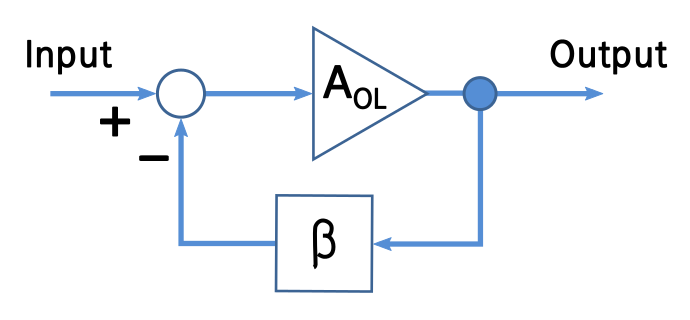
\includegraphics[width=0.5\textwidth]{img/realimentacion-negativa-bloque}
	\caption{Modelo general de realimentación negativa.}
	\label{fig:ampli_feedback}
\end{figure}


\subsection{Realimentación global}


Debido a la complejidad del circuito, cumplir con todas las especificaciones a lazo abierto es altamente complejo y requiere demasiada precisión en el cálculo y elección de componentes. Esto derivaría en un circuito altamente complejo y costoso. Es por este motivo que se emplea el realimentador. En esquema empleado se ve en la figura~\figref{fig:ampli_feedback_blocks}.

Dado que en un amplificador de audio se busca que la salida sea una versión de escalada de la señal de entrada, se busca tomar una muestra de la misma, y compararla con la señal de entrada. 

Como sabemos, si se cumple que la ganancia de lazo cumple que $a \cdot f \gg 1$, donde $a$ es la ganancia del amplificador a lazo abierto y $f$ la transferencia del realimentador, es esta última la que fija fija la ganancia a lazo cerrado, siendo la misma $A_{v} \simeq \frac{1}{f}$.

Una ventaja de esta técnica es que ayuda a que el amplificador se asemeje a un amplificador de tensión ideal, ya que aumenta la resistencia de entrada, mientras que disminuye la de salida y como la ganancia termina dependiendo de componentes pasivos, resistores y un capacitor en este caso, con la elección de la tecnología y calidad adecuadas para estos, se logra una gran estabilidad frente a variaciones de las condiciones, como ser la temperatura, esto no es así para las resistencias de entrada y salida, ya que las mismas dependen de la ganancia de lazo. 

La realimantación es muy beneficiosa siempre que sea negativa. Dado que el sistema naturalmente introduce desfasajes, para ciertas frecuencias la realimentación puede pasar de ser negativa, a ser positiva (esto haría que las diferencias entre la señal de salida real y deseada se amplifiquen en lugar de reducirse) provocando que el circuito oscile a estas frecuencias. Para evitar que el circuito se vuelva inestable, es necesario que para las frecuencias donde se invierte la fase, el circuito pase de amplificar a atenuar, si esto no ocurre naturalmente, es necesario agregar componentes adicionales para compensar el circuito y evitar que se vuelva inestable.

Otro factor a tener en cuenta, es que puede darse la aparición de frecuencias en la salida del circuito fuera del rango de las que se presentan naturalmente en la entrada (en este caso $20 \si[per-mode=symbol]{\hertz} \longrightarrow 20 \si[per-mode=symbol]{\kilo\hertz}$ por tratarse de audio). También para eliminar estos inconvenientes es que el sistema debe ser compensado.

El uso de realimentación global permite mejorar notablemente casi todas las especificaciones del amplificador y simplificar su diseño (la estabilidad como se mencionó antes es una característica que puede empeorar, siendo el Slew-rate la otra que puede empeorar debido a la necesaria compensación). En este caso, como el objetivo es armar un amplificador de tensión, utilizamos un circuito realimentador Serie-Paralelo (muestrea tensión y suma tensión). El factor de realimentación queda definido por las especificaciones de sensibilidad y potencia RMS para una carga determinada.


\begin{figure}[H]
	\centering
	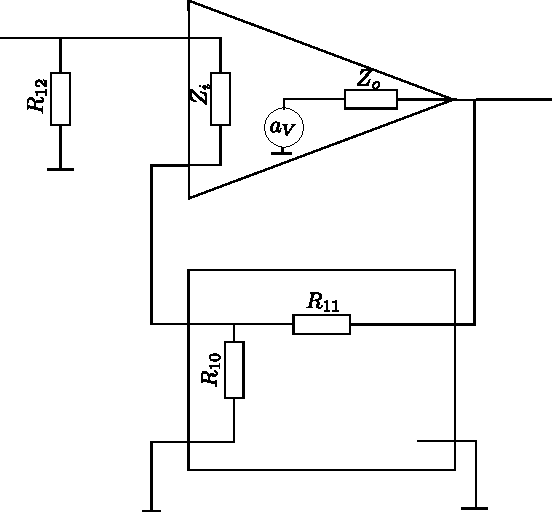
\includegraphics[width=0.5\textwidth]{img/realimentacion}
	\caption{Modelo amplificador-realimentación. El amplificador se encuentra realimentado con una topología serie-paralelo, muestreando tensión a la salida, y sumando tensión a la entrada, resultando un amplificador de ganancia de tensión estabilizado en tensión.}
	\label{fig:ampli_feedback_blocks}
\end{figure}


\subsection{Amplificador a lazo abierto}

Las etapas de un amplificador hacen referencia a su estructura a gran escala: el diagrama en bloques que modulariza los componentes y ayuda a diseñar, entender y evaluar su funcionamiento. La arquitectura de un amplificador típico consta, básicamente, de 3 etapas: una de entrada, diferencial, una intermedia, de ganancia de tensión, y una de salida, de ganancia de corriente o potencia (figura~\figref{fig:etapas}).

\begin{figure}[H]
	\centering
	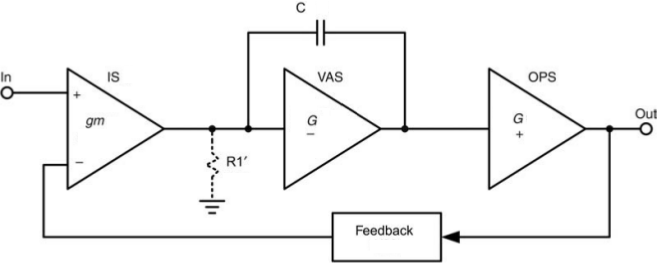
\includegraphics[width=0.6\textwidth]{img/etapas}
	\caption{Tres etapas de un amplificador típico, su realimentación y su capacitor de compensación (compensación por Miller). El esquema es genérico y no representa al amplificador diseñado.}
	\label{fig:etapas}
\end{figure}


Se han propuesto arquitecturas de dos etapas (como en \textbf{\quotemarks{\textit{Linsley-Hood, Simple Class-A amplifier , Wireless World [~April~1969~] p. 148}}} y en \textbf{\quotemarks{\textit{B. Olsson , Better audio from non-complements? Electronics World [~December~1994~] p. 988}}}) unificando la segunda y la tercera etapa. Sin embargo, dificulta el proceso de diseño sin grandes beneficios visibles, es poco común entre amplificadores comerciales, y suele ofrecer mala distorsión. También se han propuesto arquitecturas de cuatro etapas, como \textit{Lohstroh y Otala} en su paper \textbf{\quotemarks{\textit{An audio power amplifier for ultimate quality requirements}}}. Sin embargo, tampoco es muy usado en la industria, pues esta complejidad adicional no parece traer beneficios, al menos no en un amplificador discreto, es posible que no sea así en un diseño monolítico integrado.


El amplificador diseñado entonces tiene una \textbf{estructura típica de tres etapas}, aunque con la variante de ser completamente simétrico (e incluir un seguidor por emisor acoplado al VAS por razones de polarización mayormente). La última etapa es la responsable de proveer la potencia y la que determina la eficiencia, tamaño y peso del amplificador; en particular, es la etapa que le da el nombre de amplificador, en nuestro caso, \textbf{Clase G}.


\subsection{Antecedentes}

El libro de \textbf{Douglas Self}~\citelink{Douglas_Self_ENG5} compila la vasta experiencia de un diseñador de amplificadores profesional, es un libro de referencia y renombre en el mundo de los amplificadores de audio. Durante el diseño de este amplificador se tomó de referencia este libro para evaluar las opciones y sus ventajas y desventajas según la experiencia de la industria. El clase G de la figura~\figref{fig:ampli_DS} fue tomado directamente de su libro, estudiado y simulado. 

\clearpage

\begin{figure}[H]
	\centering
	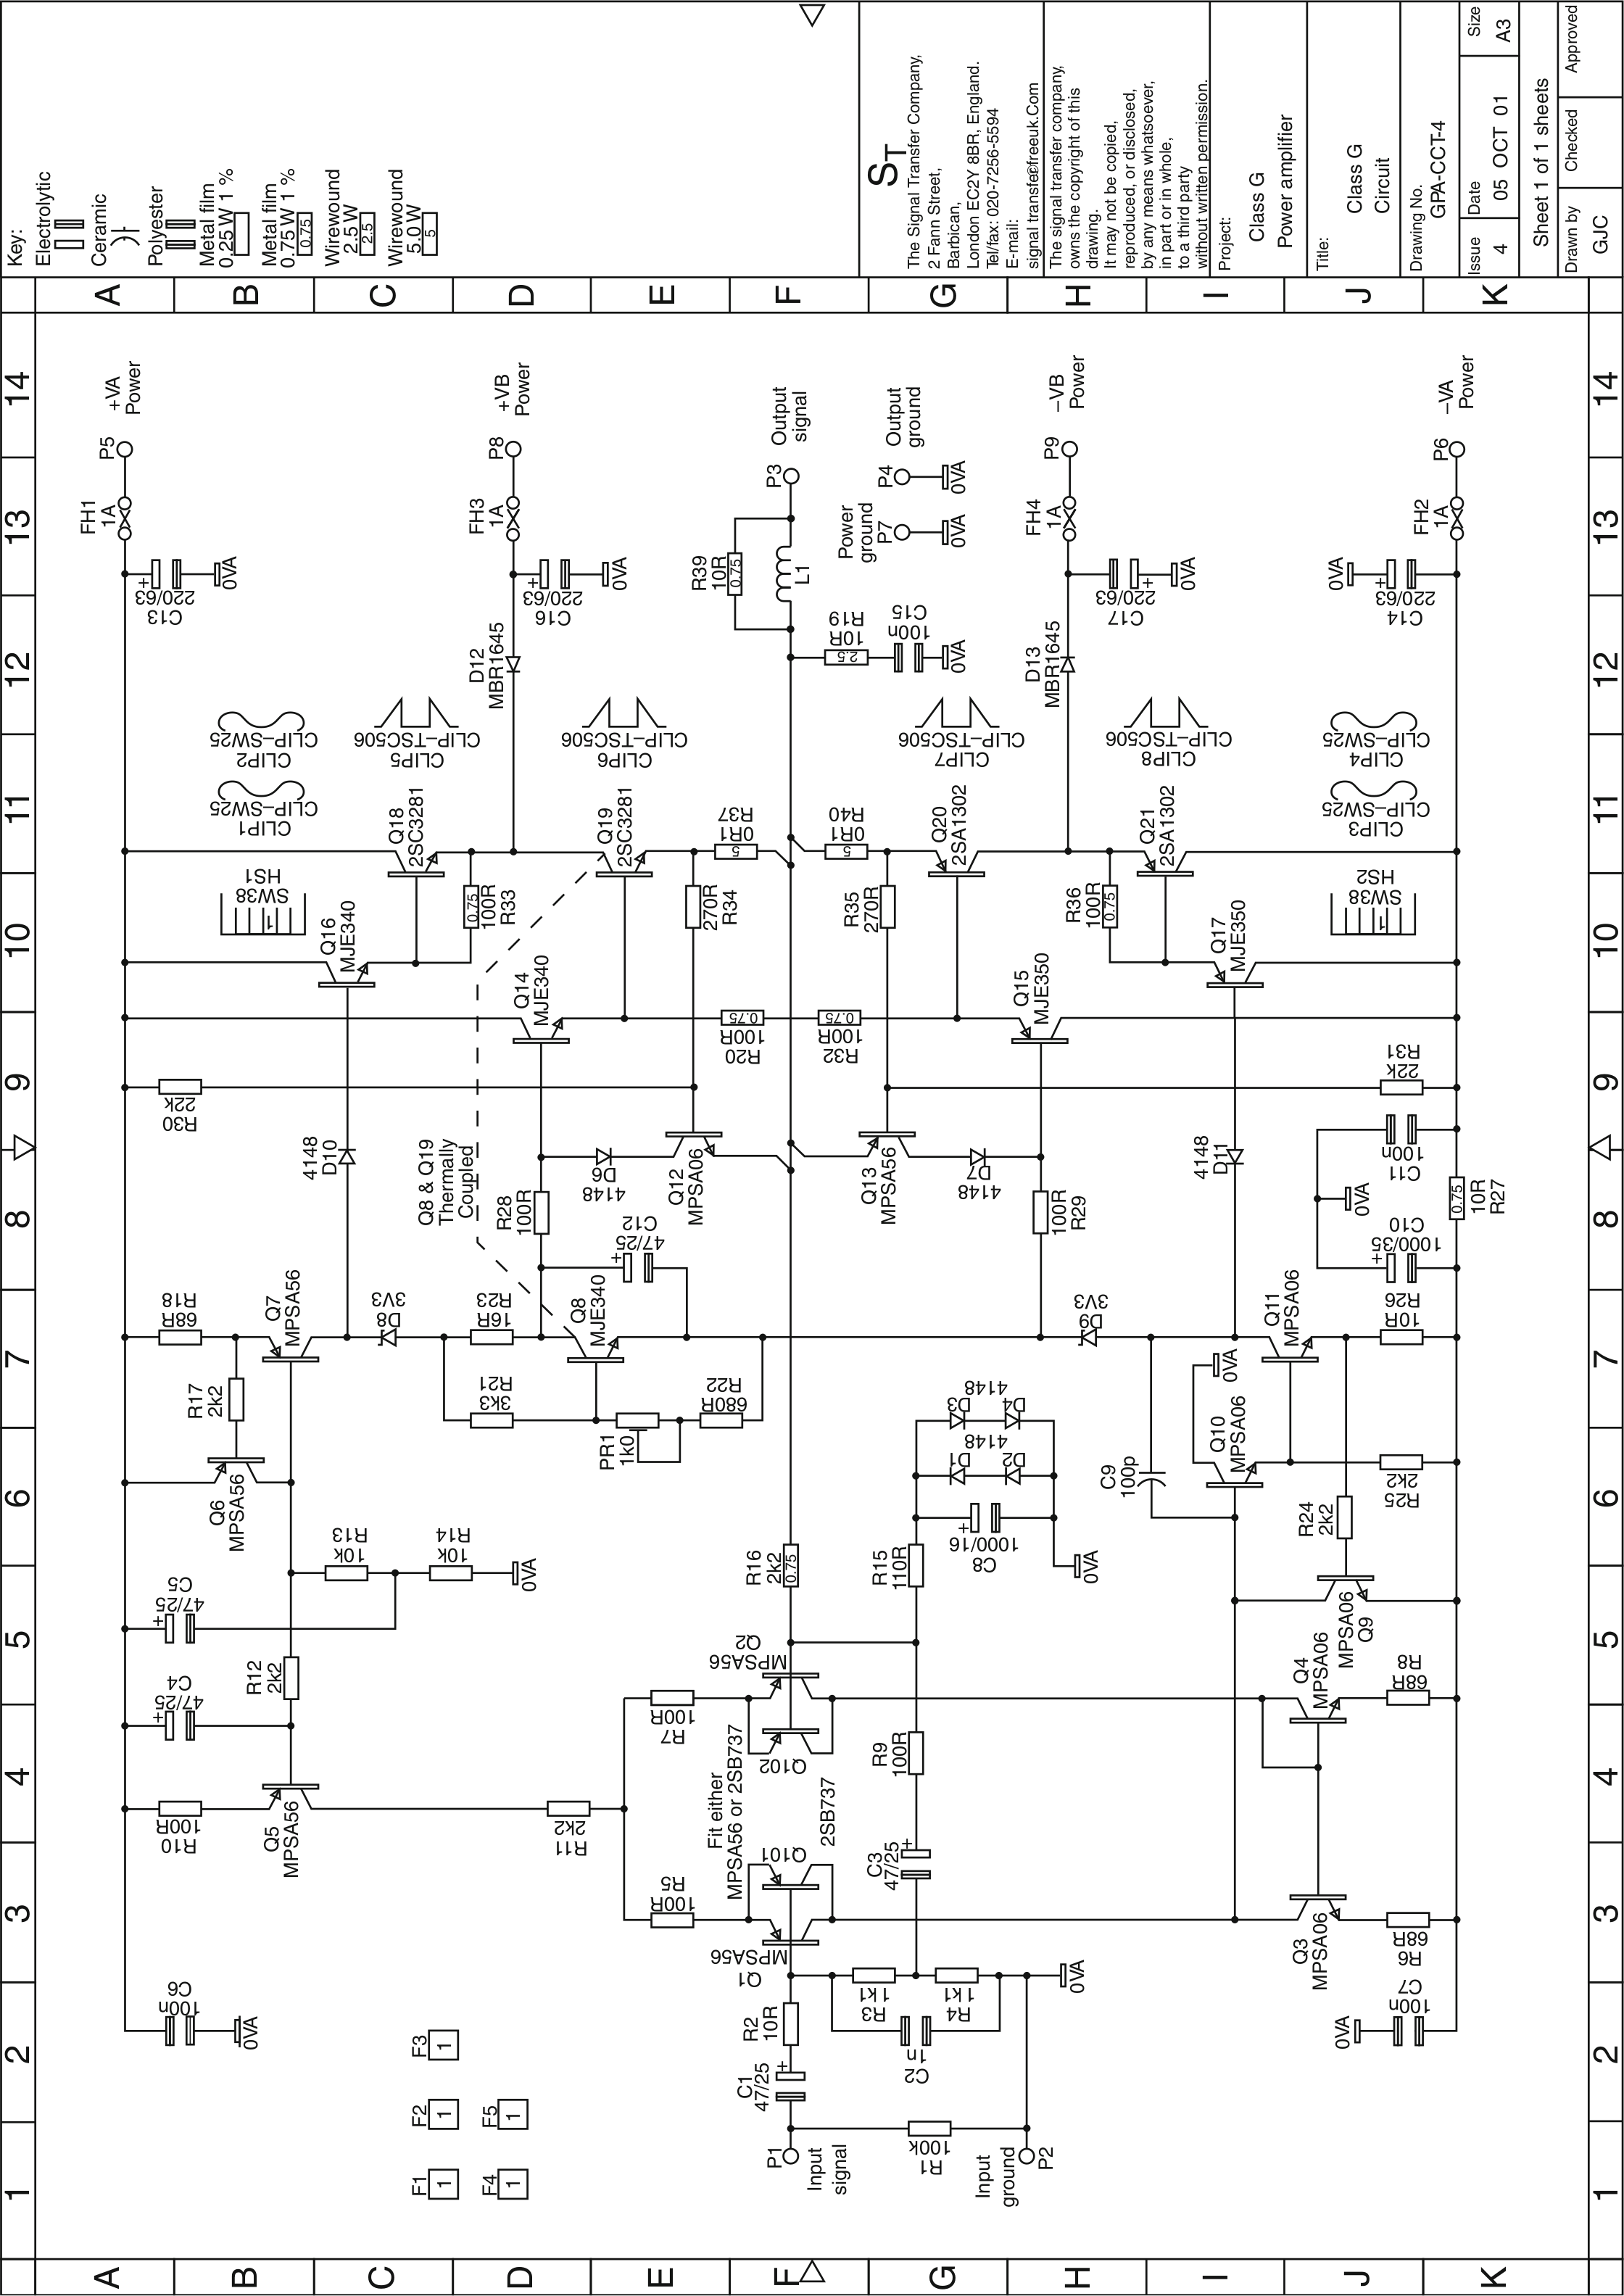
\includegraphics[width=0.86\textwidth]{img/clase_g_del_libro.png}
	\caption{Amplificador clase G, \textbf{Douglas Self}~\citelink{Douglas_Self_ENG5}}
	\label{fig:ampli_DS}
\end{figure}


\clearpage

\subsection{Etapa de entrada}

En el esquema de tres etapas, la primera cumple la función de amplificar la diferencia entre sus dos entradas, rechazando las señales comunes. Esta capacidad de rechazo de las señales comunes es importante no sólo para implementar el modelo de realimentación planteado, sino para reducir el efecto de ruidos que afecten de forma igual a ambas entradas.
Sin embargo, esta simetría no es total: el comportamiento en un semiciclo difiere del comportamiento del semiciclo opuesto, por estas mismas alinealidades mencionadas. Se eligió entonces una topología de doble par diferencial. Es decir, propusimos agregar otro par, en paralelo, con componentes complementarios: donde originalmente usamos transistores \textbf{NPN}, colocamos \textbf{PNP}, y viceversa. De esta forma, la simetría cancela mas de las alinealidades y se reduce la distorsión aún más. También se tiene la ventaja de disminuir el offset, ya que al ser complementarios los pares diferenciales, se cancelan parcialmente las corrientes de base de los transistores, y por supuesto duplicar las etapas duplica la ganancia total a lazo abierto que se obtiene. Esta decisión llevó a luego intentar mantener una simetría total en todo el circuito, llevando naturalmente al circuito completamente simétrico. 


Otra opción de diseño más, es la de la carga de los pares diferenciales. Estos pueden ser activas o pasivas. Por lo general, se elige una carga de tipo activa, como por ejemplo, una fuente de corriente espejo, porque da una menor distorsión, esto es típico en amplificadores operacionales, pero en nuestro caso, este diseño original fue descartado por consejo de los docentes, ya que, a pesar de tener un muy buen desempeño en las simulaciones, al ser implementado en la práctica presenta problemas de estabilidad en la polarización, de la charla con los docentes y posteriores simulaciones nos llevaron a elegir un amplificador tipo cascode, con una carga pasiva, porque necesitamos la caída en la carga para polarizar la etapa siguiente, donde explicaremos el motivo. 



Por último y no menos importante, es necesario determinar la forma de polarizar con corriente a los transistores de las ramas de los amplificadores diferenciales. Esto se hace mediante una fuente de corriente cuyo diseño puede tomar diversas formas: fuente espejo, semi-espejo, cascode, etc. Normalmente, se utiliza un transistor con una resistencia en serie en el emisor, y algún semiconductor en la base del transistor, para fijar una tensión de polarización, mientras la resistencia antes mencionada determina la corriente de polarización que luego se dividirá a la mitad por las ramas del diferencial. La opción elegida hace uso de un par de diodos de señal (\textbf{1N4148}) que fijan la corriente del transistor en forma bastante independiente de la tensión de alimentación. Normalmente, estas fuentes, toman la referencia desde los rieles externos, porque son más estables que los internos, pero en este caso, al ser las tensiones de los rieles externos muy elevados, preferimos utilizar unos reguladores lineales (\textbf{78L05} y \textbf{79L05}, versiones de baja corriente, $100 \si[per-mode=symbol]{\milli\ampere}$), para tomar de los rieles internos, y obtener $\pm 5 \si[per-mode=symbol]{\volt}$ de notable estabilidad, gracias al rechazo de ripple de $60 \si[per-mode=symbol]{\decibel}$ de estos reguladores. Esta tensión se usa para polarizar las bases de los base común de los cascode, es en verdad la principal motivación de estos reguladores, ya que los diferenciales son implementados con un array de transistores integrados (\textbf{MMPQ6700}) que tienen una tensión de $V_{ce}$ de ruptura baja, unos $30 \si[per-mode=symbol]{\volt}$, con los reguladores se garantiza estar en la zona segura de operación, y se tiene la ventaja de tener una polarización muy estable, cosa muy deseable en una primera etapa.


\subsection{Etapa de amplificación de tensión (VAS).}

Por lo general, la etapa de amplificación suele estar compuesta por un simple amplificador de configuración EC (Emisor Común), entrando a la etapa de salida, por debajo del multiplicador de $V_{be}$, y polarizado por una fuente de corriente de colector. En este amplificador se optó por un diseño EF VAS (Emitter Follower - VAS): a este EC con degeneración de emisor, se le agrega una etapa colector común anterior, antes del amplificador. El seguidor cumple la función de  separar la etapa de entrada, esto mejora la distorsión y aumenta la ganancia a lazo abierto al tener una mayor resistencia de entrada cargando al cascode de la primer etapa. También se puede modificar para que la salida del VAS no sea por debajo del multiplicador de $V_{be}$, sino por el medio, para disminuir el offset a la salida, previo a la realimentación, y disminuir la distorsión. El inconveniente de este modo es que se necesitan dos fuentes de corriente más, ya que el modo anterior, aprovecha la fuente de polarización del EF VAS, para polarizar, también, el multiplicador de $V_{be}$. En nuestro caso, con el cambio a 2 pares diferenciales, duplicamos la etapa EF VAS, complementariamente, y se conectan a la etapa de salida, por arriba y por abajo del multiplicador de $V_{be}$, esta simetría disminuye aún mas la distorsión. Como en este caso, cada uno de los dos EF VAS hace de carga del otro, los EF VAS no tienen fuente de polarización, entonces se necesita que la etapa diferencial tenga una carga resistiva, para fijar la tensión de base de los EF VAS, la caída en este resistor es determinada por la fuente de corriente, con lo que es bastante estable. Si hubiéramos usado una carga tipo fuente espejo, habríamos logrado que la corriente en las ramas del par diferencial fueran mas simétricas, pero sin fijar ninguna tensión estable para polarizar la base de los EF VAS, como nos hicieron notar los docentes.

\subsection{Etapa de salida}
Esta etapa es la responsable de amplificar la potencia de la señal. Es decir, debe tener \textbf{alta eficiencia}, y \textbf{bajos niveles de distorsión}. Además, se busca \textbf{minimizar la impedancia de salida} para mantener un \textbf{alto factor de amortiguamiento} y evitar que el rebote acústico afecte el comportamiento del amplificador. 
La etapa de salida \textbf{clase G} está compuesta por dos o más niveles de alimentación que permiten incrementar la eficiencia del amplificador con respecto al \textbf{clase B}. Esto se logra ya que con tensiones bajas, se utilizará una fuente de tensión menor, preservando la máxima excursión posible sobre la carga que ofrece un clase B alimentado con la fuente de tensión mayor. Para señales con picos de baja amplitud en relación al valor medio, la mejora en la eficiencia es modesta. Sin embargo, en el caso en que la señal tenga picos considerables con respecto a su valor medio, la mejora es notable. Un punto importante, a la hora de diseñar una etapa de salida clase G, es la tensión de los rieles internos. Tomamos del libro de \textbf{Douglas Self}~\citelink{Douglas_Self_ENG5}, los estudios realizados considerando los casos en los cuales la tensión de riel interno es de $30 \si[per-mode=symbol]{\percent}$ y $60 \si[per-mode=symbol]{\percent}$ del externo, y se observó que los beneficios en cuanto a eficiencia, del segundo caso, son pocos. En cambio, en el caso de rieles internos de $30 \si[per-mode=symbol]{\percent}$ respecto de los externos, la eficiencia aumenta considerablemente. Otro detalle de diseño, es la del multiplicador de $V_{be}$ doble. El multiplicador de $V_{be}$ más simple, tiene un transistor, y 2 resistores, con las que forma el salto de potencial necesario para eliminar el problema de cruce por $0$ de la etapa de salida. En este caso, se usan $2$ transistores complementarios, con la misma idea que el del doble par diferencial, para que el corrimiento de tensión del multiplicador de $V_{be}$ sea lo más lineal posible, en el libro se explica que esta configuración es especialmente adecuada para salidas tipo Darlington y se ajusta muy bien a nuestro circuito por su simetría.

\subsubsection{Protección de cortocircuito}

%%\fxnote{Tomado del Douglas, 5th ed, page 447 en adelante}

En la figura~\figref{fig:simple-current-limit} se puede ver la versión más básica de protección por sobre-corriente de los transistores de salida. Cuando la corriente es tal que la caída en $R_{e_{1}}$ supera, aproximadamente los $0.6 \si[per-mode=symbol]{\volt}$, los transistores $TR_{1}$ y $TR_{4}$ conducen y desvían corriente de la base de $TR_{2}$ . Análogamente, para el semiciclo negativo, si la caída en $R_{e_{2}}$ supera los $0.6 \si[per-mode=symbol]{\volt}$. Se muestrea corriente a través de $R_{e_{1}}$ y $R_{e_{2}}$, que funcionan como resistencias de emisor y a la vez como sensores de corriente. Los valores de estas resistencias de emisor se determinan por los requerimientos de eficiencia o estabilidad, por lo que el valor de corriente límite queda determinado por los divisores de tensión ($R_{1}$ - $R_{2}$ y el simétrico). Nuestro circuito de protección es una versión modificada de este circuito, una cosa que observamos, es que el circuito de protección introduce bastante distorsión, especialmente si la limitación de corriente es cercana a la mayor corriente que el circuito puede entregar, con lo que nos limitamos a limitar la corriente a valores seguros para los transistores de salida, no necesariamente para la fuente de alimentación, la cual se protegió en forma independiente con una combinación de limitación de corriente y fusibles, esto se explica en la sección correspondiente.


\begin{figure}[H]
	\centering
	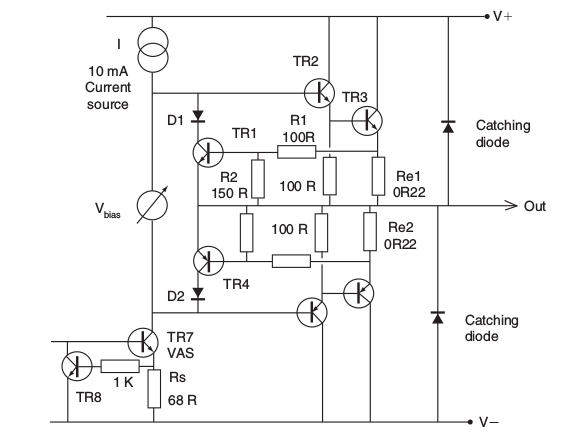
\includegraphics[width=0.6\textwidth]{img/simple-current-limit.png}
	\caption{Limitador de corriente simple}
	\label{fig:simple-current-limit}
\end{figure}



\subsection{Diagrama en bloques}

Finalmente en la figura~\figref{fig:ampli_bloques} se muestra un diagrama en bloques conceptual de nuestro circuito amplificador, mostrando en particular su estructura completamente simétrica.


\begin{figure}[H]
	\centering
	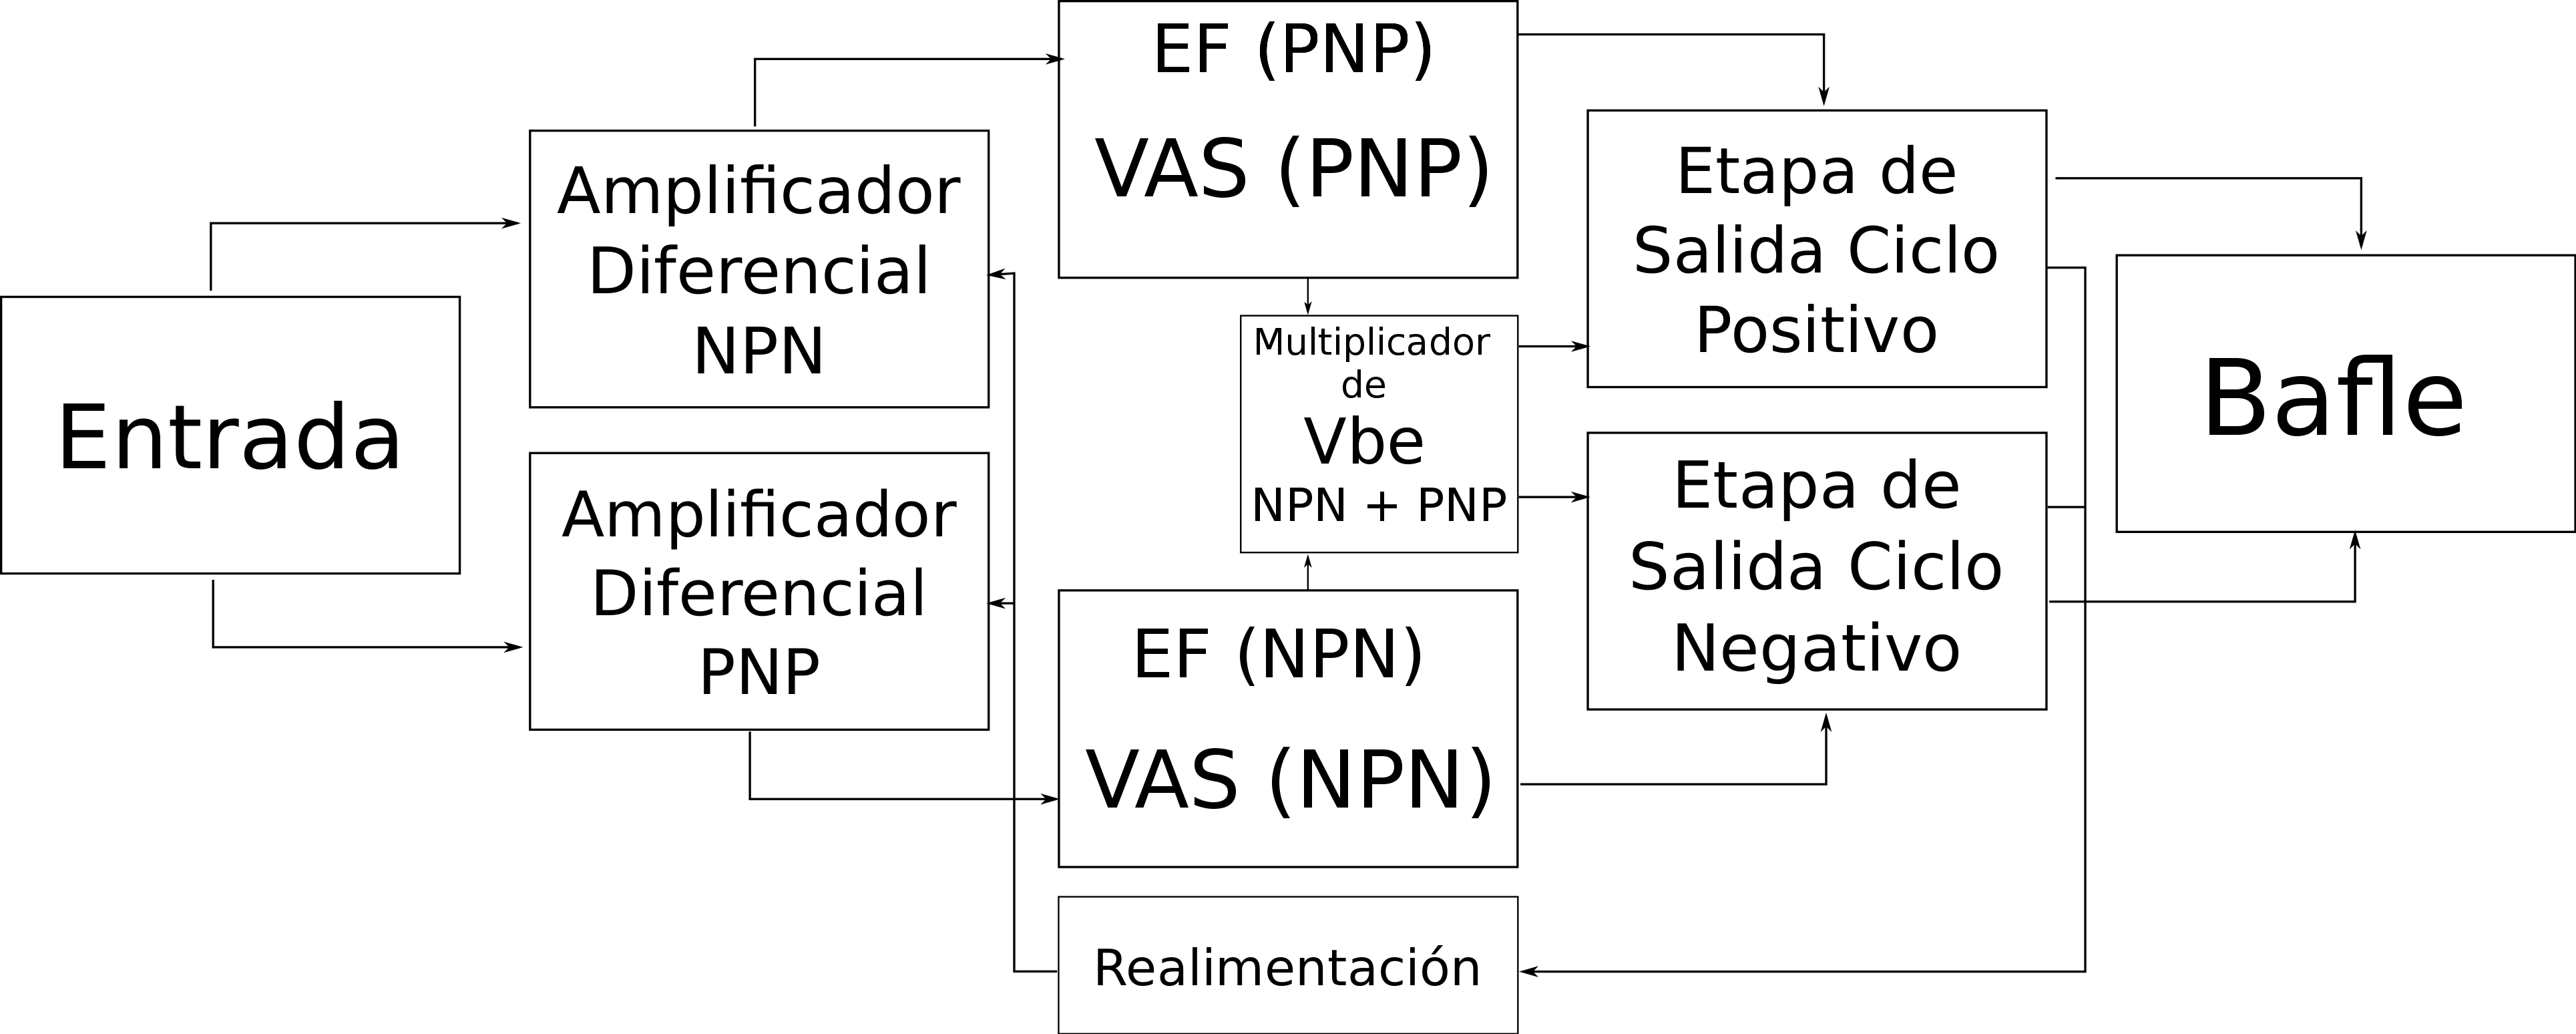
\includegraphics[width=0.75\paperwidth, angle=90]{img/bloques.png}
	\caption{Diagrama en bloques del amplificador clase G}
	\label{fig:ampli_bloques}
\end{figure}
\clearpage
%\\\\\\\\\\\\\\\\\\\\\\\\\\\


%\\\\\\\\\\\\\\\\\\\\\\\\\\\
\section{Diseño circuital}
\resetallcounters
En esta sección concretamos en circuitos reales los conceptos abstractos de la sección anterior, justificando cada parte del circuito y la elección de sus componentes.
En la figura~\figref{fig:designed_circuit} puede verse nuestro circuito amplificador completo, incluyendo el punto de trabajo de cada transistor, es el circuito que se usó en cada una de las simulaciones para validar el circuito contra las especificaciones que se establecieron. En el circuito también se marcaron algunos ratings de componentes, potencias de resistores y tensiones de capacitores, los cuales se obtuvieron de las simulaciones, estos se especificaron y se usaron a la hora de armar el listado de componentes final, teniendo en cuenta también las tecnologías adecuadas para cada componente elegido.

\clearpage


\begin{figure}[H]
\centering
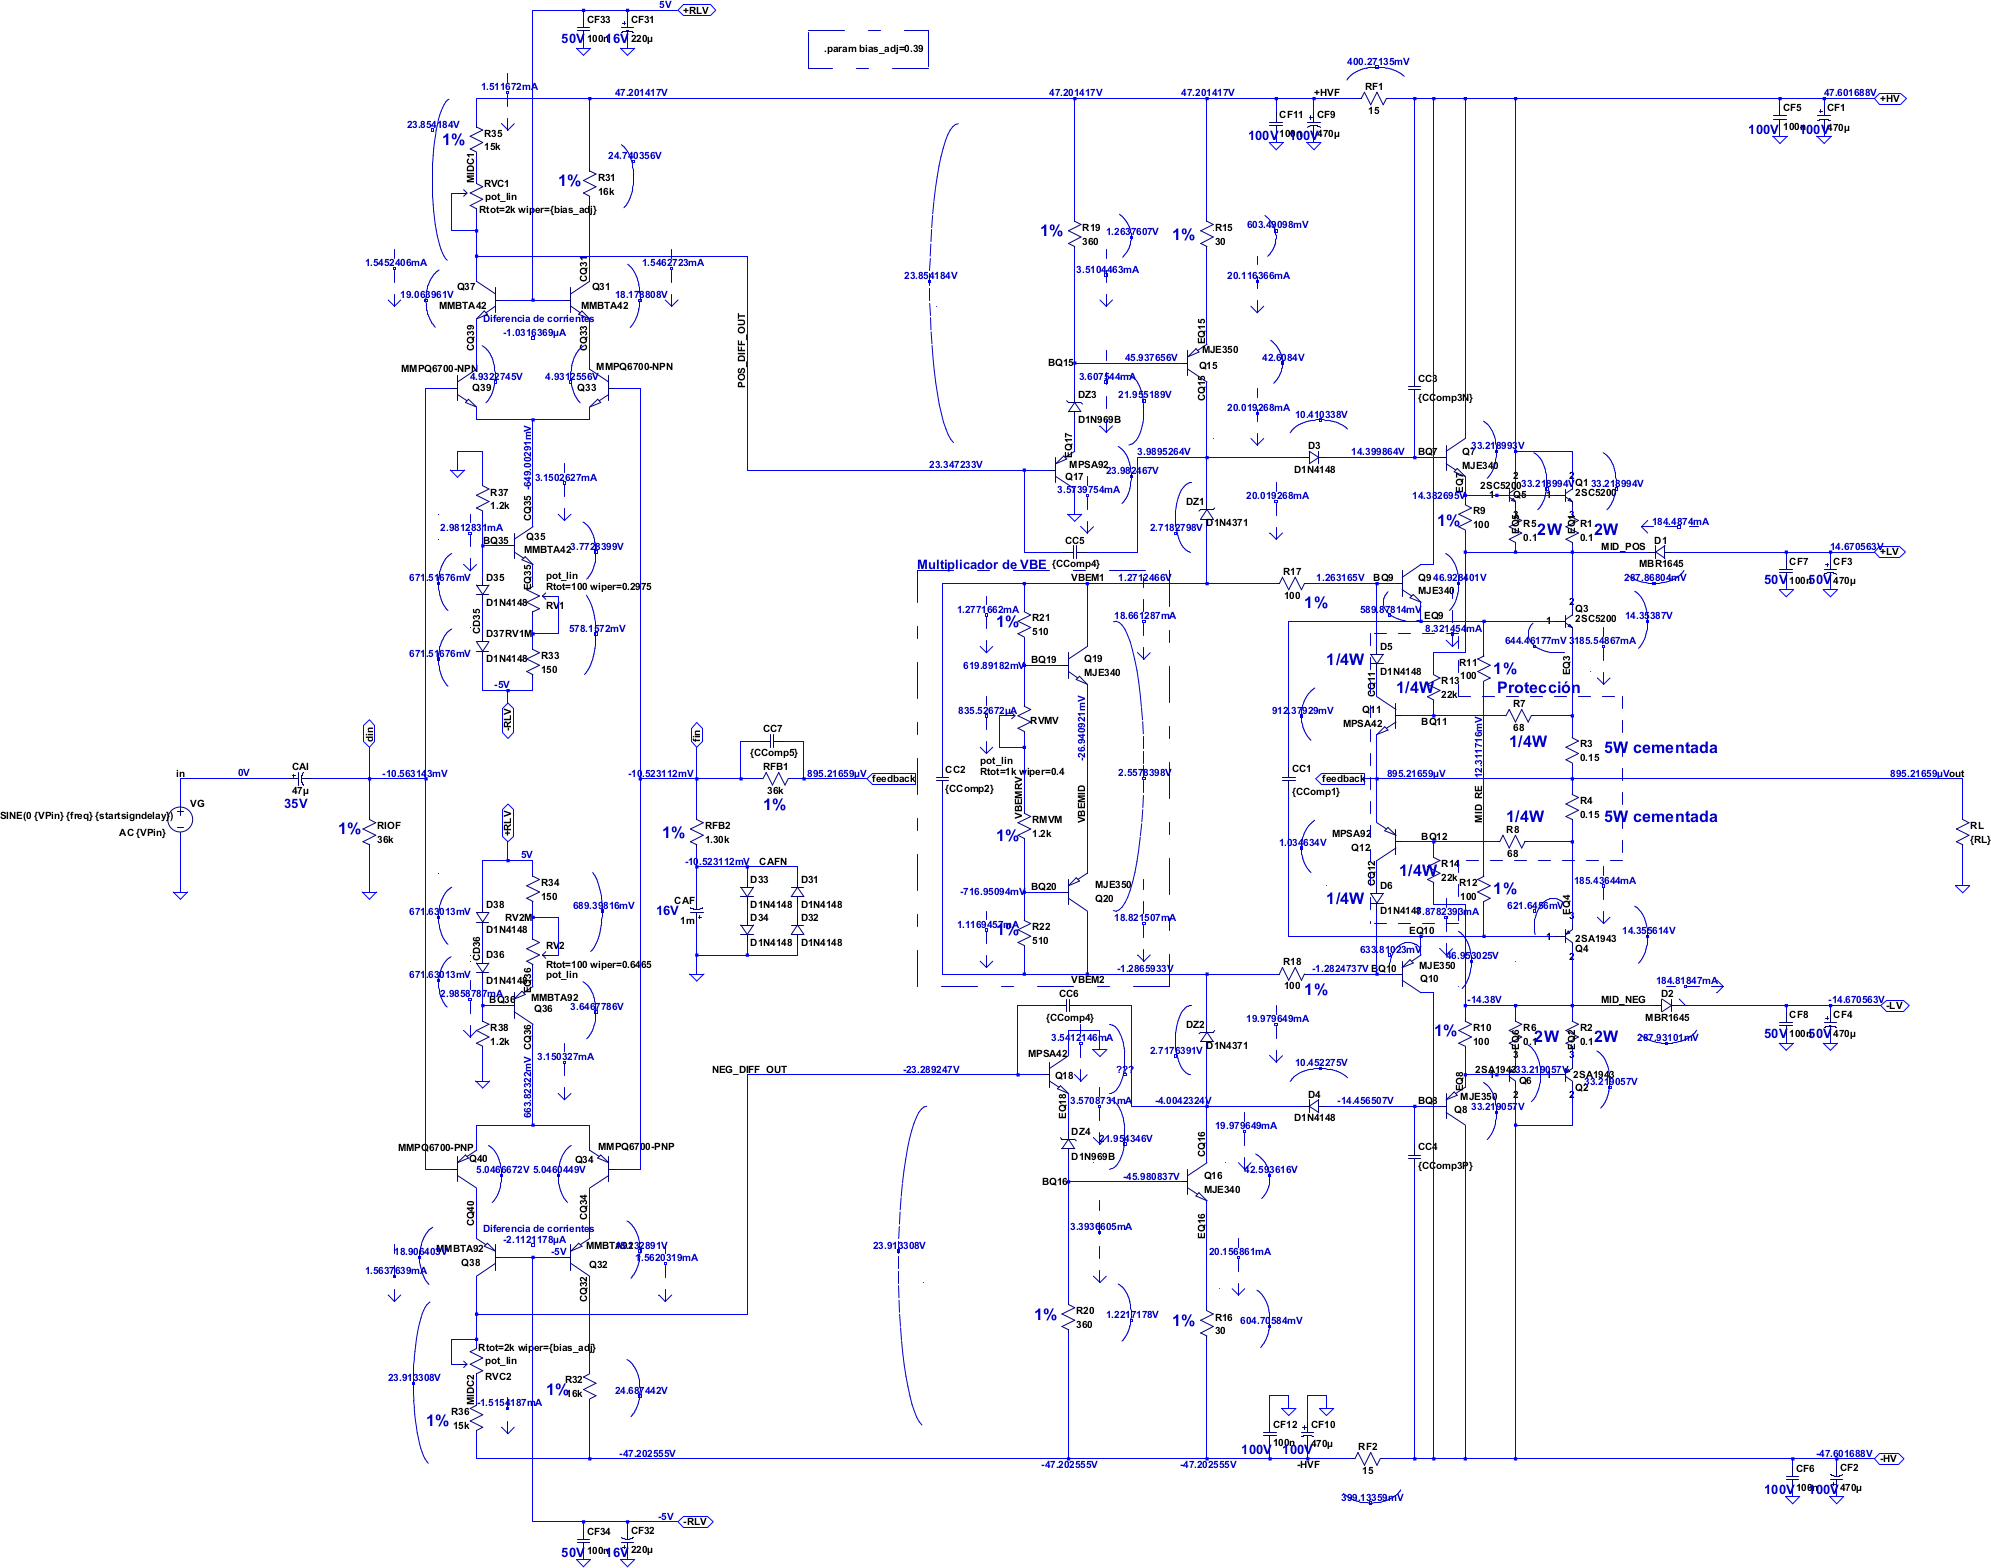
\includegraphics[width=0.9\paperwidth,angle=90,origin=c]{img/circuito.png}
\caption{Circuito Diseñado}
\label{fig:designed_circuit} 
\end{figure}

\clearpage


\subsection{Etapa de entrada}


Se usó doble par diferencial para mantener la simetría total y reducir la distorsión por armónicos pares, figura~\figref{fig:etapa-1}. Cada par se diseñó teniendo en cuenta que la tensión de salida de polarización debía ser estable, pues la segunda etapa no estará polarizada por una fuente de corriente. Por esto, los resistores de carga de los pares diferenciales ($R_{35}$, $RVC_{1}$ y $R_{36}$, $RVC_{2}$) son formadas por un resistor fijo de $15 \si[per-mode=symbol]{\kilo\ohm}$ y un preset multi-vuelta de $2 \si[per-mode=symbol]{\kilo\ohm}$, mucho menor que la resistencia dinámica de pequeña señal que le ofrece la segunda etapa ($\approx 60 \si[per-mode=symbol]{\kilo\ohm}$), dominando el paralelo. El ajuste de la polarización, consiste en ajustar primero la corriente de las fuentes de corriente y luego ajustar los presets de las cargas para lograr el punto deseado.
Por la misma razón, se consideró de particular importancia garantizar que las corrientes de polarización por las ramas del par se independicen de posibles variaciones en la segunda etapa o del riel. Los transistores $Q_{33}$~con~$Q_{39}$ y $Q_{34}$~con~$Q_{40}$, en configuración cascode combinados a $Q_{37}$~con~$Q_{31}$ y $Q_{38}$~con~$Q_{32}$ cumplen justamente la función de generar esta independencia.


\begin{wrapfigure}{R}{0.5\textwidth}
  \begin{center}
   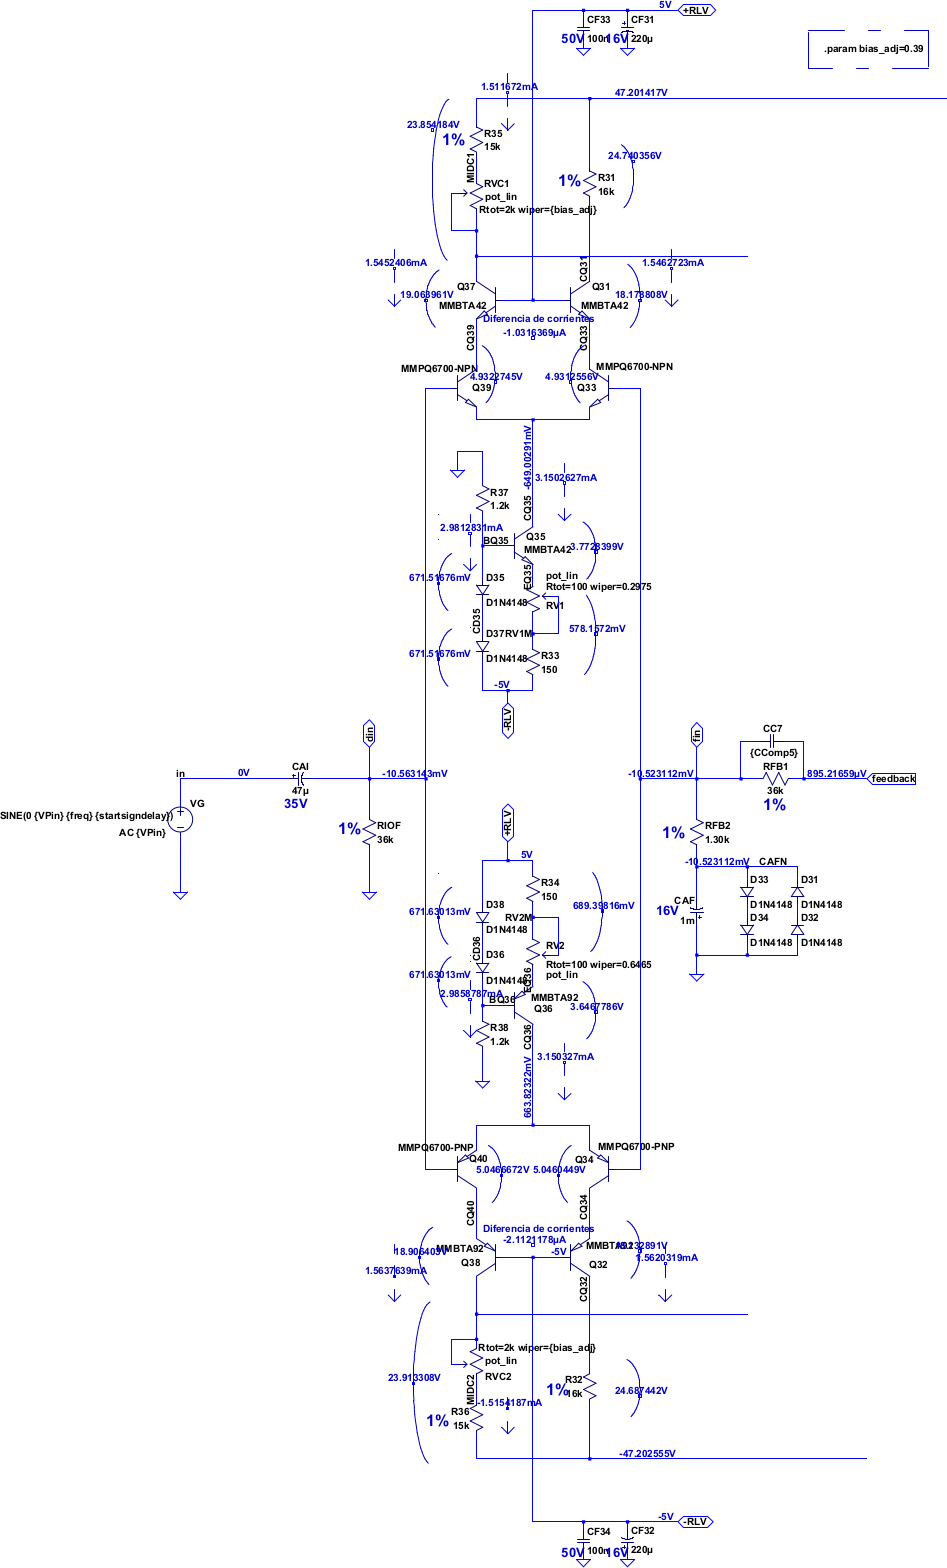
\includegraphics[width=0.4\textwidth]{img/etapa-1.png}
   \caption{Etapa primera del circuito diseñado.}
   \label{fig:etapa-1}
  \end{center}   
\end{wrapfigure}


Se polarizó cada rama con una corriente de $1.56 \si[per-mode=symbol]{\milli\ampere}$. Mayor corriente no generaría una mucho mayor amplificación de la etapa, pues, para mantener una tensión de salida fija habría sido necesario reducir la resistencia de carga en igual proporción. Esta corriente se generó con fuentes de corriente de $3.15 \si[per-mode=symbol]{\milli\ampere}$, se ajusta para que por los resistores de carga circulen $1.5 \si[per-mode=symbol]{\milli\ampere}$, logrando los $23.85 \si[per-mode=symbol]{\volt}$, independientes de la alimentación, que polarizan la segunda etapa. Los transistores de los pares diferenciales están formados cada uno por dos de los transistores de un array integrado, el \textbf{MMPQ6700}, de cuatro transistores, dos \textbf{NPN} y dos \textbf{PNP}, estos transistores como se mencionó tienen baja tensión de ruptura, pero el circuito elegido garantiza su operación segura, al ser integrados se tiene un grado alto de matcheo en sus características, esta característica se aprovecha para armar los diferenciales, dejando los base común de los cascodes a ser implementados por transistores complementarios discretos del tipo \textbf{MMBTA42}/\textbf{MMBTA92}, que son las versiones \textbf{SMD} de los conocidos transistores complementarios \textbf{MPSA42}/\textbf{MPSA92}, generalmente usados en amplificadores de potencia justamente por sus altas tensiones de ruptura y buenas características para audio.



%\begin{figure}[H]
%\centering
%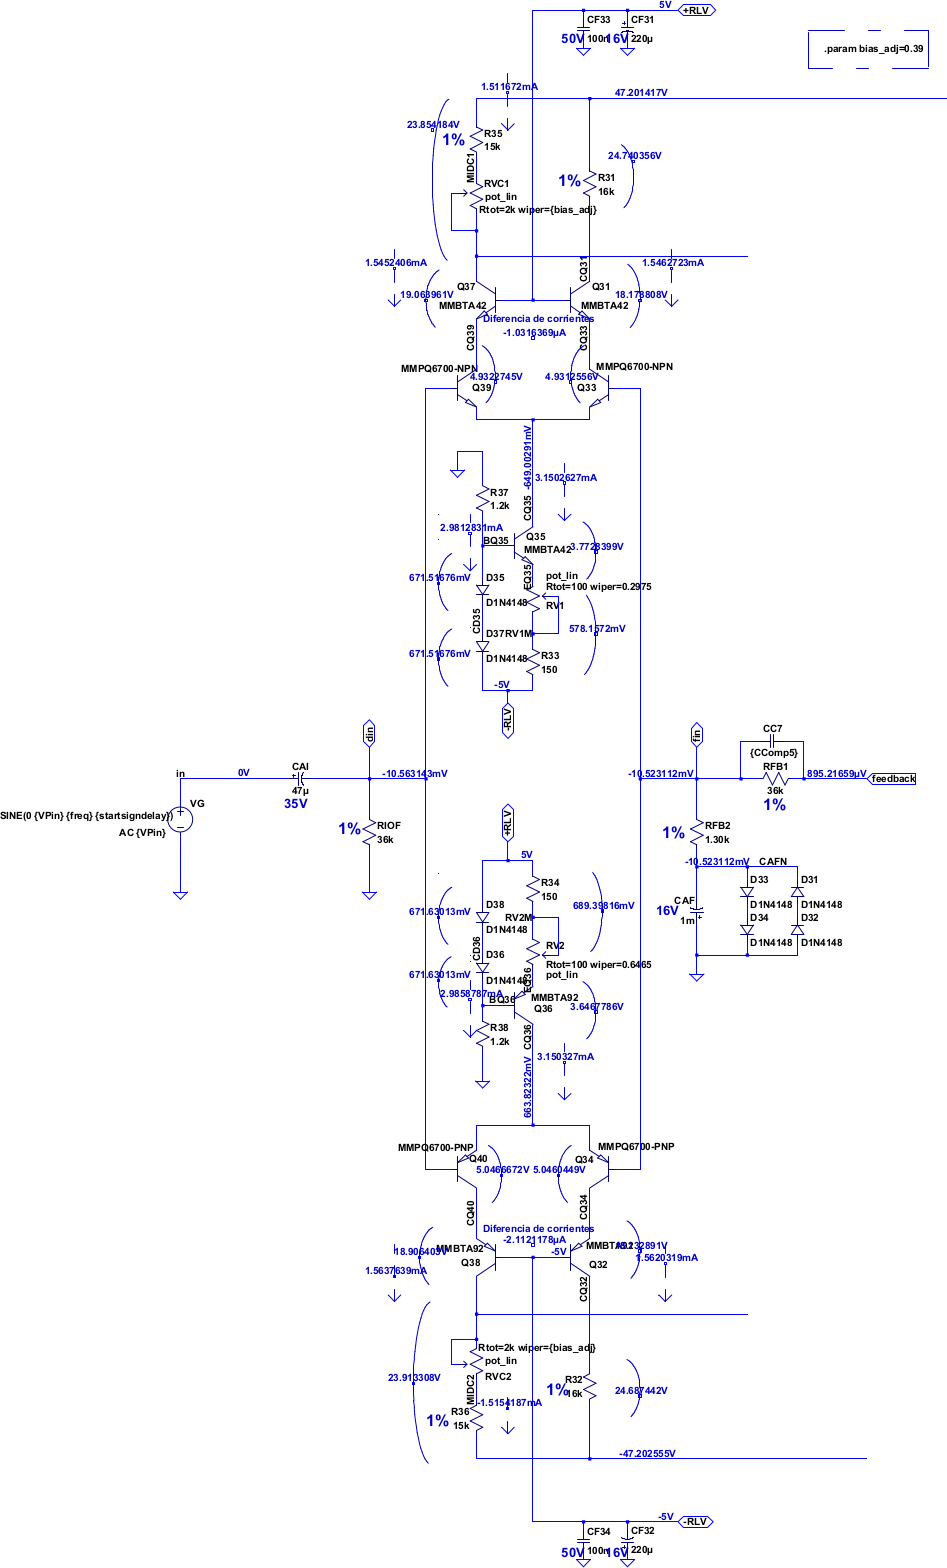
\includegraphics[width=0.36\textwidth]{img/etapa-1.png}
%\caption{Etapa primera del circuito diseñado.}
%\label{fig:etapa-1} 
%\end{figure}


\clearpage


\subsection{Etapa de amplificación de tensión}

Se optó por una configuración \textbf{CC-EC}, una para cada salida del doble par diferencial, figura~\figref{fig:vas-1}. El colector común cumple la función de ofrecer una resistencia alta a la primera etapa, independizando la polarización de los parámetros variables de los transistores de la segunda etapa. Además, aumenta la diferencia de tensión de polarización requerida entre el riel y la entrada de la etapa, lo que permite el uso de una resistencia de carga mayor en la primera etapa, mejorando su ganancia. Esta configuración, además, ofrece un alto grado de independencia de las variaciones de tensión del riel, pues todas las tensiones involucradas varían en conjunto (la única que no lo hace es masa, pero está conectada al colector de $Q_{17}$ y $Q_{18}$, nodos de alta impedancia). 


\begin{wrapfigure}{R}{0.5\textwidth}
  \begin{center}
   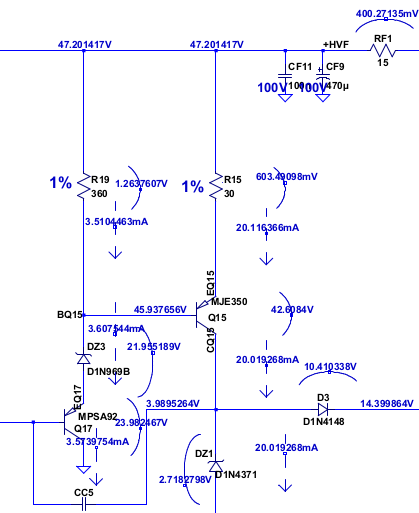
\includegraphics[width=0.4\textwidth]{img/vas-1.png}
   \caption{\textbf{VAS} en \textbf{CC-EC} del riel positivo del circuito diseñado (el otro \textbf{VAS} es perfectamente complementario).}
   \label{fig:vas-1} 
  \end{center}   
\end{wrapfigure}



%\begin{figure}[H]
%\centering
%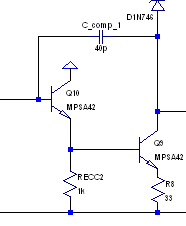
\includegraphics[width=0.3\textwidth]{img/sim/vas-1}
%\caption{VAS en CC-EC del riel negativo del circuito diseñado.}
%\label{fig:vas-1} 
%\end{figure}

Las resistencias de emisor de los \textbf{EC}, $R_{15}$ y $R_{16}$, implementan realimentaciones locales que estabilizan la corriente de polarización y ganancia de la etapa. Son realimentaciones \textbf{serie-serie} (muestrean corriente y suman tensión), estabilizando la transconductancia de la etapa. Son de valor reducido pues al estabilizar la ganancia, la reducen. Además, la caída de tensión en estas resistencias reduce la máxima excursión de la etapa antes de que saturen los transistores al mismo tiempo que determinan la corriente de colector. Se eligieron los valores exactos (junto con los de las cargas de la primera etapa) para que la corriente de polarización sea $20 \si[per-mode=symbol]{\milli\ampere}$.

Las resistencias $R_{19}$ y $R_{20}$ aseguran una corriente de polarización del colector común $3.5 \si[per-mode=symbol]{\milli\ampere}$. De no existir, la polarización podría ser muy baja, y dependiente de las variabilidades del $\beta$ del transistor del \textbf{EC}. Esta baja corriente implicaría, además, un $r_{d}$ grande, y esto es indeseable: El \textbf{EC} es un amplificador de conductancia y, como tal, funciona mejor recibiendo una señal de entrada de baja impedancia por su base.

Los transistores elegidos para los \textbf{VAS}, los complementarios \textbf{MJE340}/\textbf{MJE350}, de potencia media, que son lo mismos usados como drivers en la etapa de salida, fueron elegidos porque a pesar de que la corriente en esto transistores es moderada, su caída $V_{ce}$ es alta, haciendo que disipen potencias en el orden de $1 \si[per-mode=symbol]{\watt}$, estas potencias están fuera del rango adecuado para transistores de señal como son el par \textbf{MPSA42}/\textbf{MPSA92} utilizados en los seguidores, la potencia que disipan los pone justo en el límite de poder funcionar sin disipador, es posible que decidamos ponerles pequeños disipadores individuales a estos transistores.


En este punto es adecuado explicar el circuito pasa-bajos que se encuentra en los rieles de tensión alta que alimentan la primer y segunda etapa, estos simples pasa-bajos formados por un resistor y un par de capacitores, $RF_{1}$ con $CF_{9}$ y $CF_{11}$ en el riel positivo y $RF_{2}$ con $CF_{10}$ y $CF_{12}$ en el negativo, filtran el ripple de la fuente de alimentación (de $100 \si[per-mode=symbol]{\hertz}$), para eso el capacitor electrolítico de $470 \si[per-mode=symbol]{\micro\farad}$, que junto al resistor tienen una frecuencia de corte de $22.6 \si[per-mode=symbol]{\hertz}$, el capacitor cerámico de $100 \si[per-mode=symbol]{\nano\farad}$ está para filtrar el ruido de alta frecuencia que pueda filtrarse por los rieles de alimentación, principalmente debido a efectos causados por el switcheo de la etapa de salida. En general este filtrado reduce considerablemente el rechazo de de ripple de la fuente y también comprobamos que reduce un poco la distorsión, esto último es mas difícil de explicar.
Algo mas a mencionar de esta etapa, es que para adecuar la polarización del emisor común se utilizó en ambas ramas un zener de $22 \si[per-mode=symbol]{\volt}$, los mismos para la señal presentan a frecuencias medias solo una pequeña resistencia dinámica, por supuesto su capacidad parásita, afectará a altas frecuencias, pero las simulaciones indican que no perjudica al funcionamiento del circuito.

\clearpage


\subsection{Multiplicador de $V_{be}$}


El multiplicador de $V_{be}$ se diseñó con dos transistores, figura~\figref{fig:mvbe}, para mantener la simetría total del circuito y dado que, como ya se mencionó es adecuada para una etapa de salida con Darlingtons. La corriente de polarización de los transistores del VAS es $\cong 20 \si[per-mode=symbol]{\milli\ampere}$, y esta puede tener una excursión máxima de aproximadamente $4 \si[per-mode=symbol]{\milli\ampere}$ pico-a-pico. Es decir, el multiplicador debe lograr polarizarse con corrientes de $\cong 18 \si[per-mode=symbol]{\milli\ampere}$. Las simulaciones muestran que se logra una mayor estabilidad en la tensión si los transistores están polarizados con corrientes bajas. Por lo tanto, se eligió $RVMV$ tal que circule una corriente $< 19 \si[per-mode=symbol]{\milli\ampere}$, pero siempre del orden de los $\si[per-mode=symbol]{\milli\ampere}$. Se podría haber elegido un valor más cercano a $20 \si[per-mode=symbol]{\milli\ampere}$, pero una simulación remplazando al multiplicador por un generador de tensión ideal mostró que el funcionamiento y la distorsión del circuito no se veían afectados. 


\begin{wrapfigure}{R}{0.42\textwidth}
  \begin{center}
   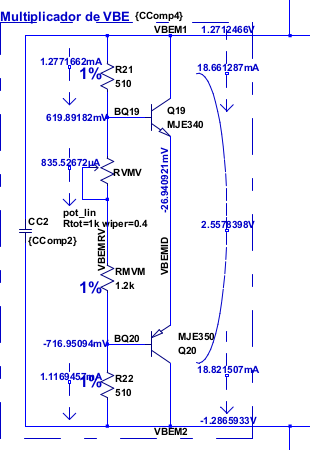
\includegraphics[height=0.5\textwidth]{img/mvbe.png}
   \caption{Multiplicador de $V_{be}$ simétrico utilizado.}
   \label{fig:mvbe}  
  \end{center}   
\end{wrapfigure}


Por esta misma razón, no se agregaron resistores adicionales en los colectores, que usualmente se usan para generar una caída que compense el incremento de tensión con la corriente. Puede hacerse como posible optimización.

Las resistencias $R_{21}$ y $R_{22}$ se eligieron iguales por simetría, y de valor tal que la tensión generada sea levemente superior a $2.5 \si[per-mode=symbol]{\volt}$. Esto permite colocar a los transistores de salida en modo levemente \textbf{A-B}, reduciendo la distorsión de su etapa.
De todas formas la manera de determinar en la práctica el valor adecuado de tensión del multiplicador, es ir aumentando la caída hasta que ya no baja la distorsión armónica, habiéndose eliminado por completo la distorsión de cruce por cero.\\
Los transistores utilizados son el par complementario \textbf{MJE340}/\textbf{MJE350}, los mismos de los VAS y drivers de la etapa de salida, son transistores de potencia media,  tienen encapsulado \textbf{TO-225}, adecuados para montar en un disipador, en este caso el motivo principal de su elección, ya que se podrían utilizar transistores de señal dado el nivel de disipación que tienen.



%\begin{figure}[H]
%\centering
%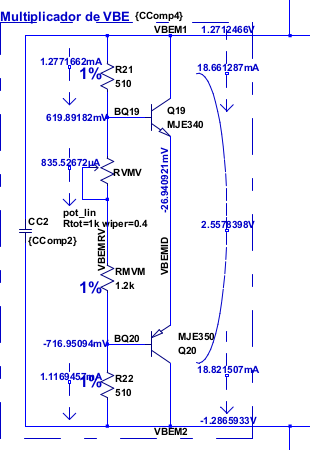
\includegraphics[height=0.5\textwidth]{img/mvbe.png}
%\caption{Multiplicador de $V_{be}$ simétrico utilizado.}
%\label{fig:mvbe} 
%\end{figure}


\clearpage



\subsection{Etapa de salida}

La etapa de salida, figura~\figref{fig:output_stage}, a pesar de parecer lo mas complicado, y ser lo primero que se diseña, es lo que menos problemas causó para determinar un circuito satisfactorio, es la única parte del circuito que no cambió a lo largo de las varias iteraciones del circuito global del amplificador, solo se le agregó el circuito de protección, del cual se probaron distintas configuraciones. Las simulaciones fueron muy satisfactorias con varios circuitos distintos en las primeras etapas, la elección correcta de los transistores de potencia fue crítica, y tener modelos proveídos por el fabricante ayudó a validar el diseño.
Se usan transistores en configuración Darlington, para tener una ganancia de corriente elevada, y con transistores en paralelo en los exteriores para repartir la corriente y disminuir la disipación en cada uno. Se colocaron los resistores $R_{1}$, $R_{5}$, $R_{2}$ y $R_{6}$ de valor $0.1 \si[per-mode=symbol]{\ohm}$ para ayudar a que se reparta de forma equilibrada la potencia entre los transistores de potencia $Q_{1}$-$Q_{5}$ y $Q_{2}$-$Q_{6}$ y estabilizarlos térmicamente, estos resistores se determinaron de $2\si[per-mode=symbol]{\watt}$, con lo cual se trata de resistores de carbón o metal de encapsulado un poco mayor al resto de los resistores de $0.25\si[per-mode=symbol]{\watt}$. Los transistores usados como drivers de los Darlington son los mismos para los internos como para los externos, se trata del par complementario \textbf{MJE340}/\textbf{MJE350}, el mismo utilizado en los VAS y el multiplicador de $V_{be}$, son de media potencia, con encapsulado \textbf{TO-225}, adecuados para poner en un disipador de ser necesario, estos transistores llevan un resistor de degeneración de emisor de $100 \si[per-mode=symbol]{\ohm}$, $R_{9}$ y $R_{10}$ para los drivers externos y $R_{11}$ y $R_{12}$ para los internos, algo interesante de estos resistores, es que en lugar de quedar conectados al punto de salida de conexión de la carga, se conectan uno con el otro salteando la conexión intermedia, esta configuración se observó en algunos circuitos comerciales simétricos, así como en el libro, las simulaciones demuestran que disminuye la distorsión armónica, aunque la explicación es difícil, aunque parece deberse a realimentación cruzada que solo es efectiva en estos circuitos completamente simétricos. 
Los transistores de salida $Q_{1}$-$Q_{5}$ y $Q_{2}$-$Q_{6}$, están todos formados por los pares complementarios \textbf{2SC5200}/\textbf{2SA1943} de la marca \textbf{Toshiba}, estos transistores de potencia, de encapsulado \textbf{TO-264}, están especialmente diseñados para amplificadores de potencia de hasta $100 \si[per-mode=symbol]{\watt}$, y son usados por \textbf{Toshiba} en sus propios amplificadores de potencia, son transistores de potencia rápidos, muy adecuados para una etapa clase G, tienen una corriente máxima de $15 \si[per-mode=symbol]{\ampere}$ y una tensión máxima de $V_{ce}$ de $230 \si[per-mode=symbol]{\volt}$. Los transistores de potencia internos necesitaban al igual que los externos unos resistores de degenaración de emisor de $0.1 \si[per-mode=symbol]{\ohm}$, sin embargo para que las protecciones limiten la corriente máxima a un valor alrededor de los $10 \si[per-mode=symbol]{\ampere}$, estos resistores se eligieron de $0.15 \si[per-mode=symbol]{\ohm}$ de $5 \si[per-mode=symbol]{\watt}$ del tipo de alambre cementado, los típicos bloques de color blanco, estos valores permiten soportar la máxima corriente por el tiempo necesario para que actúen las protecciones de la fuente de alimentación, en las condiciones normales de operación no disipan una potencia demasiado significativa, su principal perjuicio es aumentar la resistencia de salida del amplificador a lazo abierto.
El uso de los diodos Schottky \textbf{MBR1645}, el tipo de diodo, es simplemente debido a la baja caída que poseen, en el orden de $0.2 \si[per-mode=symbol]{\volt}$ para corrientes significativas, y el hecho que son rápidos, debido a no tener gran cantidad de carga acumulada como un diodo común, permitiendo que pasen rápidamente de conducción a cortados, el uso de ese específico diodo es debido a que no se observó diferencias con otros diodos similares, y se observó que estos en particular eran usados en varios circuitos comerciales, además de conseguirse fácilmente. Todos los rieles de alimentación altos y bajos, positivos y negativos para la etapa de potencia se encuentran filtrados por capacitores electrolíticos de $470 \si[per-mode=symbol]{\micro\farad}$, para filtrar el ripple y por capacitores cerámicos de $100 \si[per-mode=symbol]{\nano\farad}$ para compensar efectos inductivos que se traducen en señales de alta frecuencia que pueden afectar al circuito, especialmente las primeras etapas.


%\begin{wrapfigure}{L}{0.6\textwidth}
%  \begin{center}
%   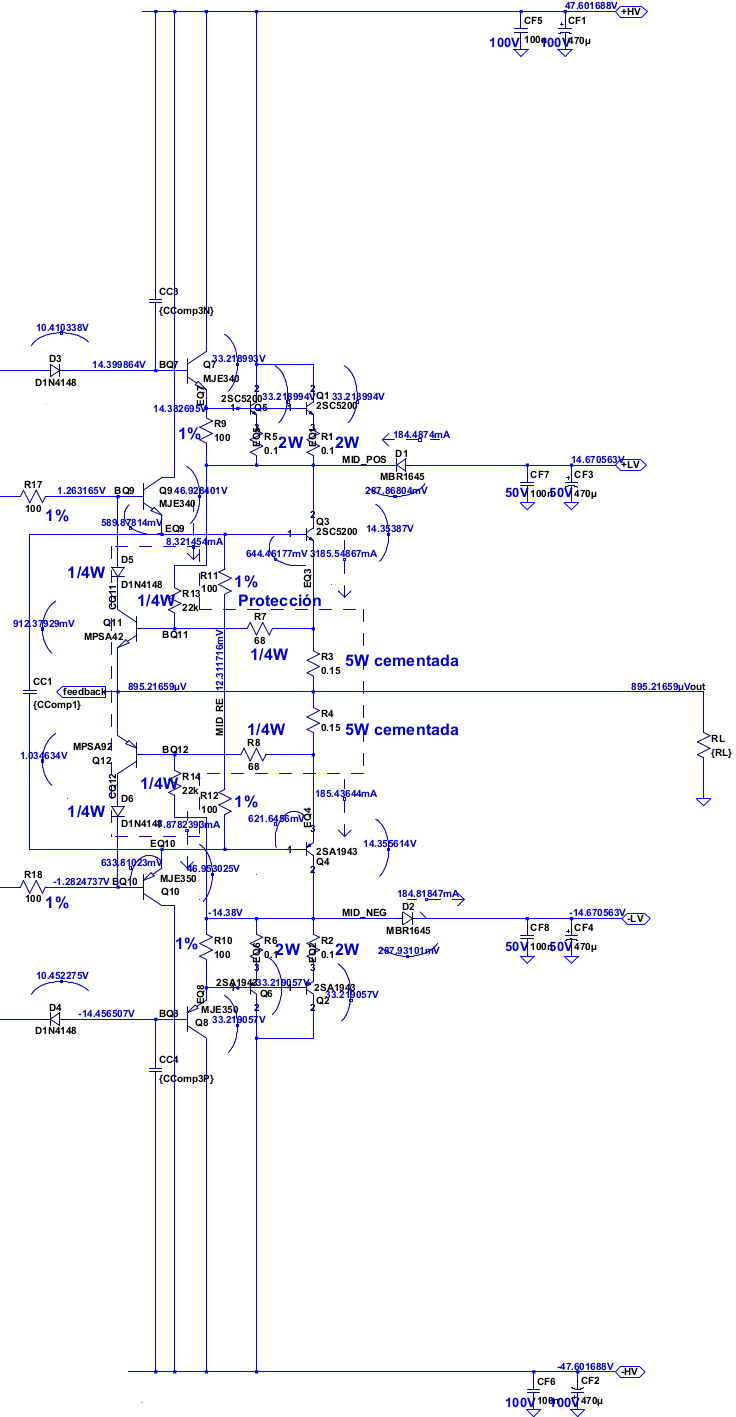
\includegraphics[height=0.5\paperheight]{img/output_stage.png}
%   \caption{Etapa de salida.}
%   \label{fig:output_stage}  
%  \end{center}   
%\end{wrapfigure}


\begin{figure}[H]
\centering
   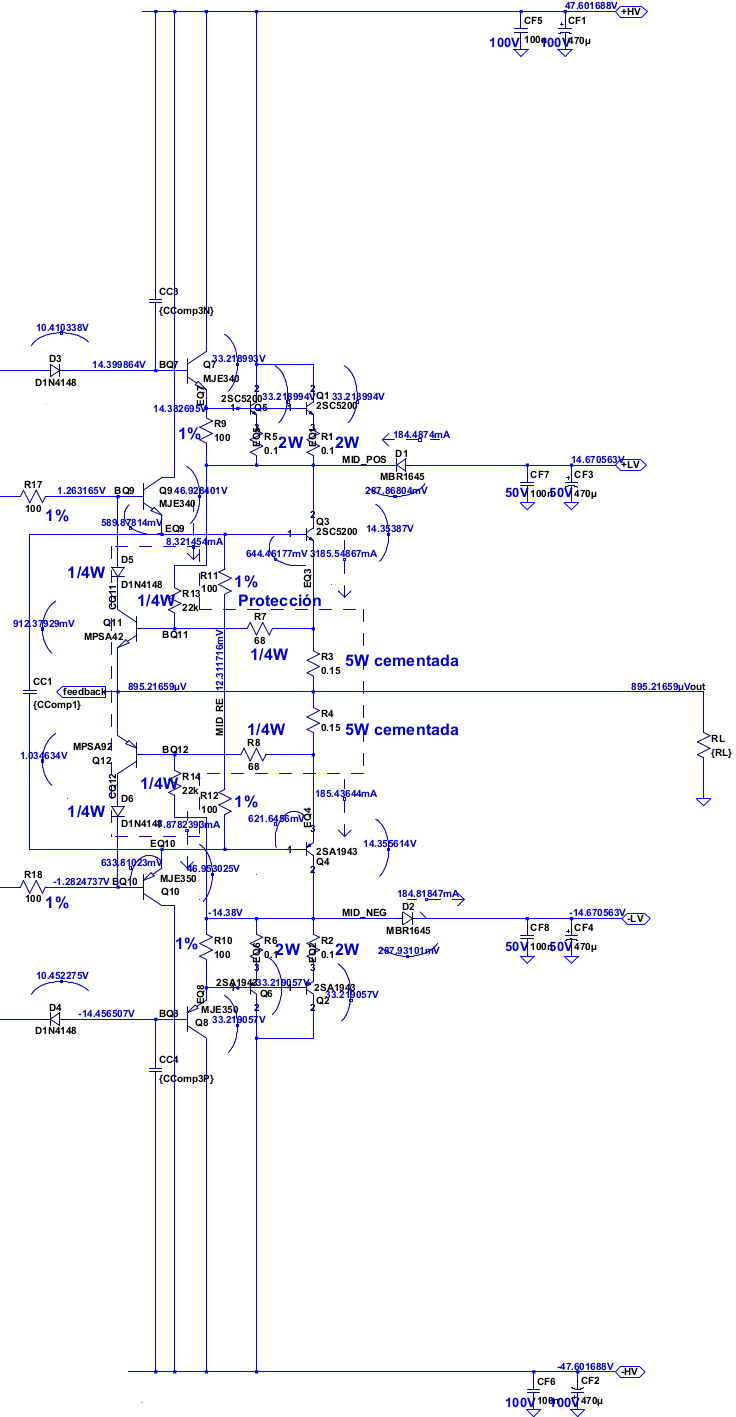
\includegraphics[height=0.66\paperheight]{img/output_stage.png}
   \caption{Etapa de salida.}
   \label{fig:output_stage}  
\end{figure}



\clearpage



\subsection{Realimentador}

Como se había mencionado en el diseño conceptual, el factor de realimentación queda definido por las especificaciones de sensibilidad y potencia RMS que definen la ganancia. Para nuestras especificaciones, la ganancia del amplificador debe ser de $29 \si[per-mode=symbol]{\decibel}$ y por lo tanto el realimentador debe atenuar $-29 \si[per-mode=symbol]{\decibel}$. Se implementa mediante un divisor de tensión que muestrea tensión y suma tensión. Deben ser resistencias lo suficientemente altas para que no afecten la salida al muestrear, y ya que para compensar el offset se usa un valor igual en la otra entrada de los diferenciales, uno de los resistores impone también la resistencia de entrada. Con una carga de $8 \si[per-mode=symbol]{\ohm}$, esto es sencillo. Por otra parte, la corriente que entra a la base del par diferencial de la primera etapa debe ser despreciable frente a la que circula por el realimentador para no afectar al factor $f$. Los valores usados se ven en la figura~\figref{fig:realimentacion-global}, los resistores se seleccionaron en valores cercanos a lo necesario dentro de los valores comerciales que se consiguen al $1 \si[per-mode=symbol]{\percent}$ de tolerancia, la tecnología seleccionada es metal film u oxide metal film, esto garantiza buena estabilidad con la temperatura y bajo ruido, cosa esencial en la red de realimentación.

\begin{figure}[H]
	\centering
	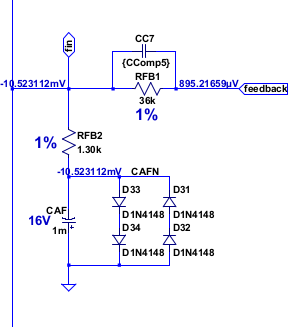
\includegraphics[width=0.4\textwidth]{img/realimentacion-global.png}
	\caption{Realimentación global implementada, junto con su compensación por atraso de fase.}
	\label{fig:realimentacion-global}
\end{figure}
 
 El capacitor $CAF$ cumple la función de modificar la realimentación en continua, a un factor unitario, y generar una simetría en las resistencias que ven las bases de los pares diferenciales de la primera etapa, y así reducir la tensión de offset. Por esta misma razón, la resistencia en paralelo a la entrada $RIOF$, que permite la polarización de $Q_{39}$ y $Q_{40}$ es del mismo valor que $RFB_{1}$.
 

Consideremos el diagrama de la figura~\figref{fig:ampli_realimentacion}. Para hallar los valores de impedancia de entrada y salida, primero debemos reflejar las resistencias $RFB_{1}$ y $RFB_{2}$, como vemos en el siguiente diagrama.

\begin{figure}[H]
	\centering
	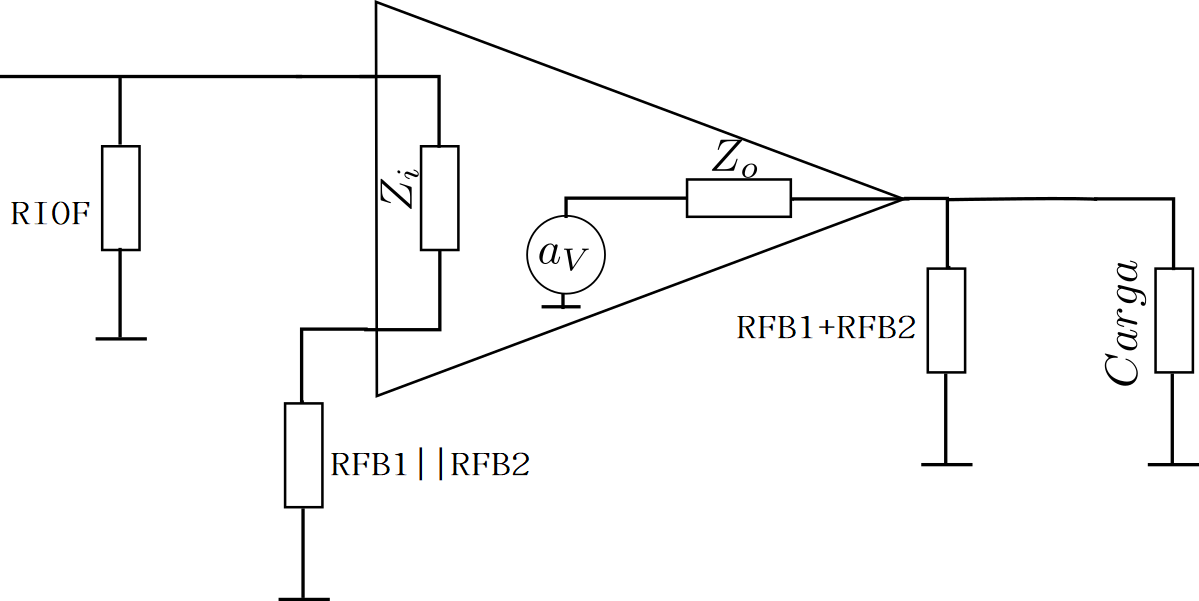
\includegraphics[width=0.5\textwidth]{img/reflejo.png}
	\caption{Modelo amplificador-reflejando resistencias}
	\label{fig:ampli_realimentacion}
\end{figure}


\begin{sloppypar}

Este amplificador tiene una amplificación de tensión a lazo abierto, de $76.35 \si[per-mode=symbol]{\decibel}$, con una impedancia de salida de aproximadamente $6 \si[per-mode=symbol]{\ohm}$.
La realimentación tiene un valor de ${ f = \frac{RFB_{2}}{RFB_{1} + RFB_{2}} \rightarrow f = 0.035 }$, resultando ${T = 1 + a_{V} \cdot f = 1 + 6569 \times 0.035 = 229.95}$. La ganancia a lazo cerrado es ${ A \cong \frac{1}{f} = 28.69 }$. En cuanto a la impedancia de entrada, $RFB_{1}$ y $RFB_{2}$ se reflejan en paralelo entre ellas, en serie a la impedancia de entrada del amplificador $Z_i$. Dada la relación entre las resistencias, $RFB_{1}$ resulta despreciable, y a su vez, $RFB_{2}$ resulta despreciable en serie con $Z_i$, que resulta despreciable, en paralelo con $RIOF$, de $36 \si[per-mode=symbol]{\kilo\ohm}$. Para la resistencia de salida, tenemos la resistencia reflejada $RFB_{1} + RFB_{2}$, que es despreciable en paralelo con $Z_o || R_{Carga} = 3.42 \si[per-mode=symbol]{\ohm}$. Luego ${ \frac{3.42}{(1 + a_{V} \times f)} = 0.01 \si[per-mode=symbol]{\ohm} }$, que es la impedancia de salida resultante. La impedancia de entrada incrementada en la ganancia de lazo resulta ser mucho mayor a $36 \si[per-mode=symbol]{\kilo\ohm}$. En nuestro circuito, la resistencia $RIOF$ de valor $36 \si[per-mode=symbol]{\kilo\ohm}$ en paralelo a la entrada del amplificador a lazo cerrado que domina la impedancia de entrada final.

\end{sloppypar}



\subsection{Compensación}

Un sistema realimentado puede sufrir de pérdidas de estabilidad debido al desfasaje que se produce en la señal. Si para algunas frecuencias se produce una inversión de fase y la ganancia es unitaria o mayor entonces el sistema pasa a estar realimentado positivamente para dichas frecuencias y oscila o se desestabiliza.

Para analizar la estabilidad del sistema es necesario analizar la ganancia a lazo abierto $T(j\omega)$. Un sistema adquiere la capacidad de oscilar si para una frecuencia dada $\omega_{k}$ se da que $T(j\omega_{k})=-1$ y se vuelve inestable si $\left| T(j\omega_{k}) \right| > 1 \; \land \; \angle T(j\omega_k) < -180 \si[per-mode=symbol]{\degree}$.

Para esta clase de análisis es útil trazar el bode de la ganancia de lazo e identificar el margen de ganancia (\textbf{MG}) y de fase (\textbf{MF}), ver figura \figref{fig:margenes}.


\begin{figure}[H]
	\centering
	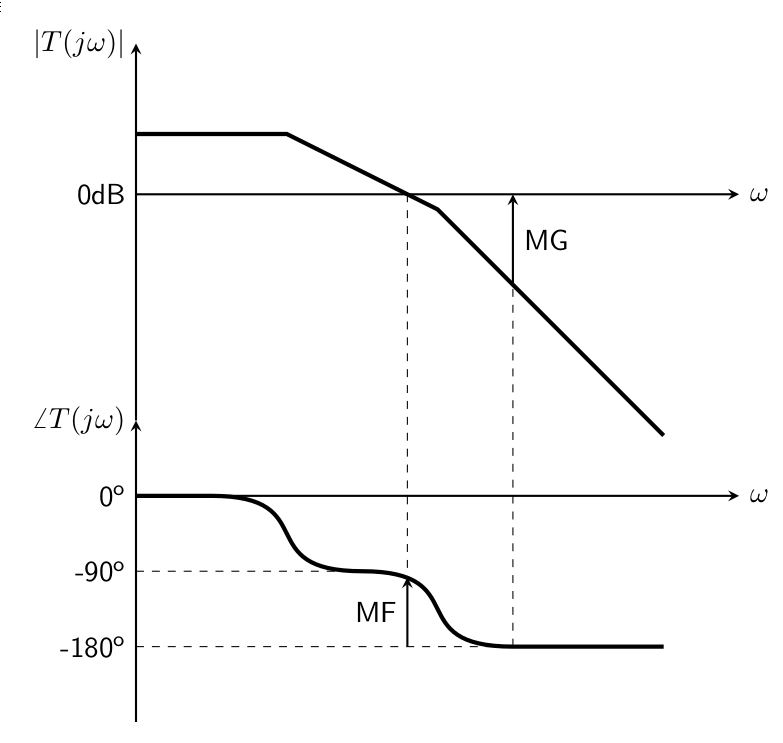
\includegraphics[height=0.35\textwidth]{img/margenes.png}
	\caption{Bode - margen de fase y ganancia.}
	\label{fig:margenes}
\end{figure}


Lo que representan estos margenes es lo siguiente:


\begin{description}
	\item[Margen de Ganancia] \hfill \\
		Representa la ganancia que habría que agregar (sumar en caso de $ \si[per-mode=symbol]{\decibel}$) para volver inestable al sistema, se mide entonces la diferencia entre $0 \si[per-mode=symbol]{\decibel}$ y la ganancia para la frecuencia en que la fase se invierte $180 \si[per-mode=symbol]{\degree}$. Si $\mathrm{MG} \le 0 \si[per-mode=symbol]{\decibel}$ entonces el sistema es inestable.

	\item[Margen de Fase] \hfill \\
		Es el desfasaje que habría que agregar al sistema para volverlo inestable, se mide entonces el ángulo que le resta a la fase por llegar a $ -180 \si[per-mode=symbol]{\degree}$ al tener ganancia unitaria.
\end{description}

Si el margen de fase o ganancia son muy bajos o negativos, es necesario corregir, modificar el circuito para que no haya una inversión de fase en ninguna frecuencias que se amplifique en el lazo, por medio de su compensación.


\begin{figure}[H]
	\centering
	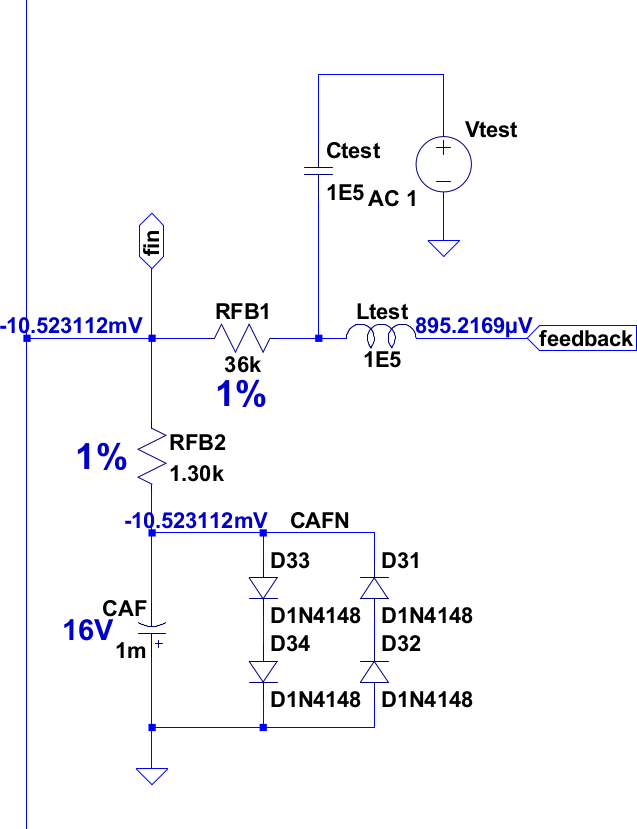
\includegraphics[height=0.35\textwidth]{img/sims/ala}
	\caption{Se abre el lazo anulando la realimentación en señal.}
	\label{fig:ala}
\end{figure}


Se realizó una simulación a lazo abierto, figura~\figref{fig:ala}, abriendo el lazo usando un capacitor y un inductor de valor grande. Luego se se midió la salida para obtener una simulación de la ganancia de lazo, figura~\figref{fig:bode-la-sin-comp}.




\clearpage

\begin{figure}[H]
	\centering
	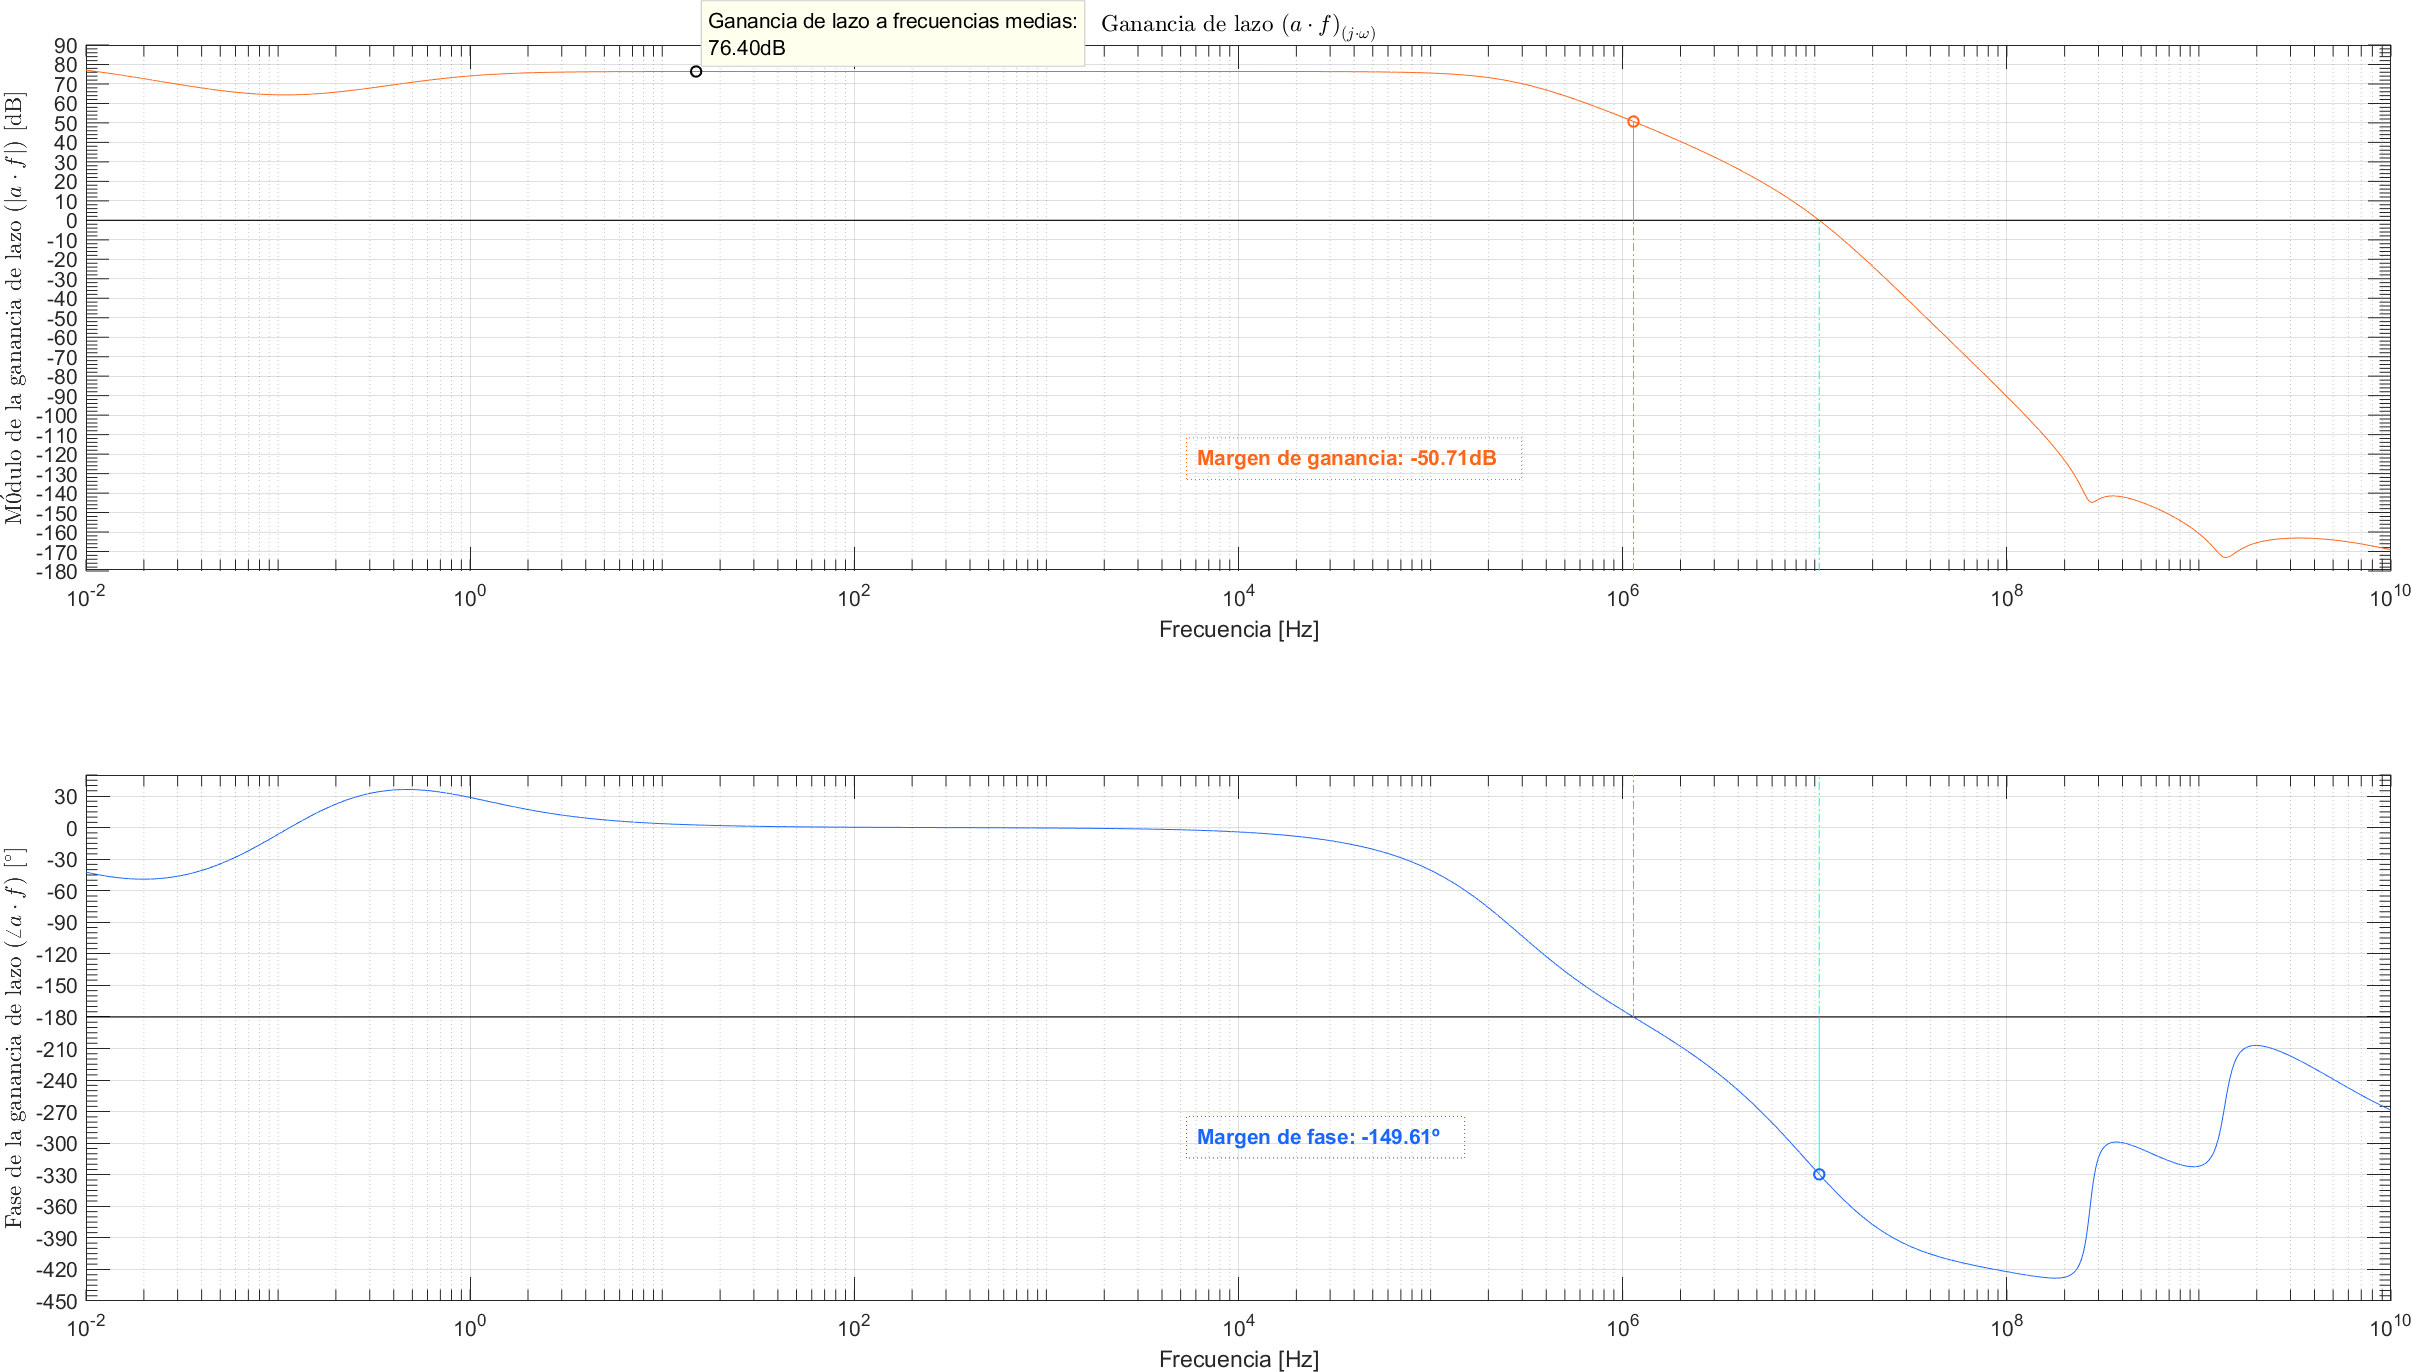
\includegraphics[width=0.85\paperwidth, angle=90]{img/sims/gain_loop_NC.png}
	\caption{Bode de la ganancia de lazo sin compensación.}
	\label{fig:bode-la-sin-comp}
\end{figure}

\clearpage



Se puede apreciar unos márgenes negativos que es necesario compensar. El polo dominante se ubica en aproximadamente $193 \si[per-mode=symbol]{\kilo\hertz}$ y corresponde al nodo entre la segunda y tercera etapa: a los colectores de $Q_{15}$ y $Q_{16}$. El margen de ganancia es de $\cong -50.7 \si[per-mode=symbol]{\decibel}$. Desplazando al polo dominante una década y media hacia las frecuencias más bajas (hasta $6.1 \si[per-mode=symbol]{\kilo\hertz}$) se llega a un margen de ganancia nulo, pues un polo hace decaer la ganancia en $20dB$ por década. Sin embargo, el polo correspondiente a los nodos de entrada de la segunda etapa (bases de $Q_{17}$ y $Q_{18}$) puede desplazarse a $6.1 \si[per-mode=symbol]{\kilo\hertz}$ con capacidades de menor valor, casi sin desplazar el polo en $193 \si[per-mode=symbol]{\kilo\hertz}$, aprovechando el efecto Miller. 
La resistencia de estos nodos está dominada por la de carga de los pares diferenciales ($RVC_{1} + R_{35}$ y $RVC_{2} + R_{36}$), de valor $16 \si[per-mode=symbol]{\kilo\ohm}$. Siendo $\frac{1}{2 \pi \cdot R \cdot C}$ la frecuencia del polo, se obtiene $C \cong 100 \si[per-mode=symbol]{\nano\farad}$. Ahora bien, si la capacidad se coloca, en vez de contra masa, contra la salida de la etapa (colectores de $Q_{15}$ y $Q_{16}$), se puede usar una capacidad desde $50 \si[per-mode=symbol]{\pico\farad}$, pues la etapa tiene una amplificación de alrededor de $62 \si[per-mode=symbol]{\decibel}$ o $1260$ veces. 

Se partió de ese valor como piso, se fue ajustando por simulación, y finalmente se colocaron capacitores ($CC_{5}$ y $CC_{6}$) de $100 \si[per-mode=symbol]{\pico\farad}$. Esto da un margen de fase de $80 \si[per-mode=symbol]{\degree}$ y un ancho de banda de $\cong 850 \si[per-mode=symbol]{\kilo\hertz}$. Estos capacitores limitan el Slew-Rate, pero se observó que para valores menores a $150 \si[per-mode=symbol]{\pico\farad}$ el Slew-Rate se encontraba por arriba de los $10 \si[per-mode=symbol]{\volt\per\micro\second}$ necesarios para el ancho de banda de potencia especificado, y para valores menores a $120 \si[per-mode=symbol]{\pico\farad}$, sobre los $15 \si[per-mode=symbol]{\volt\per\micro\second}$ especificados. Por otra parte, incrementar este capacitor reduce la ganancia de lazo en frecuencias altas y, por lo tanto, los beneficios que esto trae a la distorsión, resistencias de entrada y salida, etc. Se optó por un valor de capacidades, con margen, que podría eventualmente reducirse.

Luego, se agregó un capacitor en paralelo al realimentador ($CC_{7}$) para mejorar levemente estas especificaciones. Esto agrega un cero seguido de un polo. Por ejemplo, para la frecuencia del cero, la fase se incrementa en $45 \si[per-mode=symbol]{\degree}$ y la ganancia aumenta sólo en $3 \si[per-mode=symbol]{\decibel}$, por lo que el ancho de banda se verá incrementado levemente y el margen de fase significativamente. Se comprobó simulando que ubicar el cero en $4 \si[per-mode=symbol]{\mega\hertz}$ es un buen valor. Esto se obtiene con una capacidad de $1.2 \si[per-mode=symbol]{\pico\farad}$. El bode resultante de la ganancia de lazo compensado se muestra en la figura~\figref{fig:bode-la-con-comp}.


\clearpage

\begin{figure}[H]
	\centering
	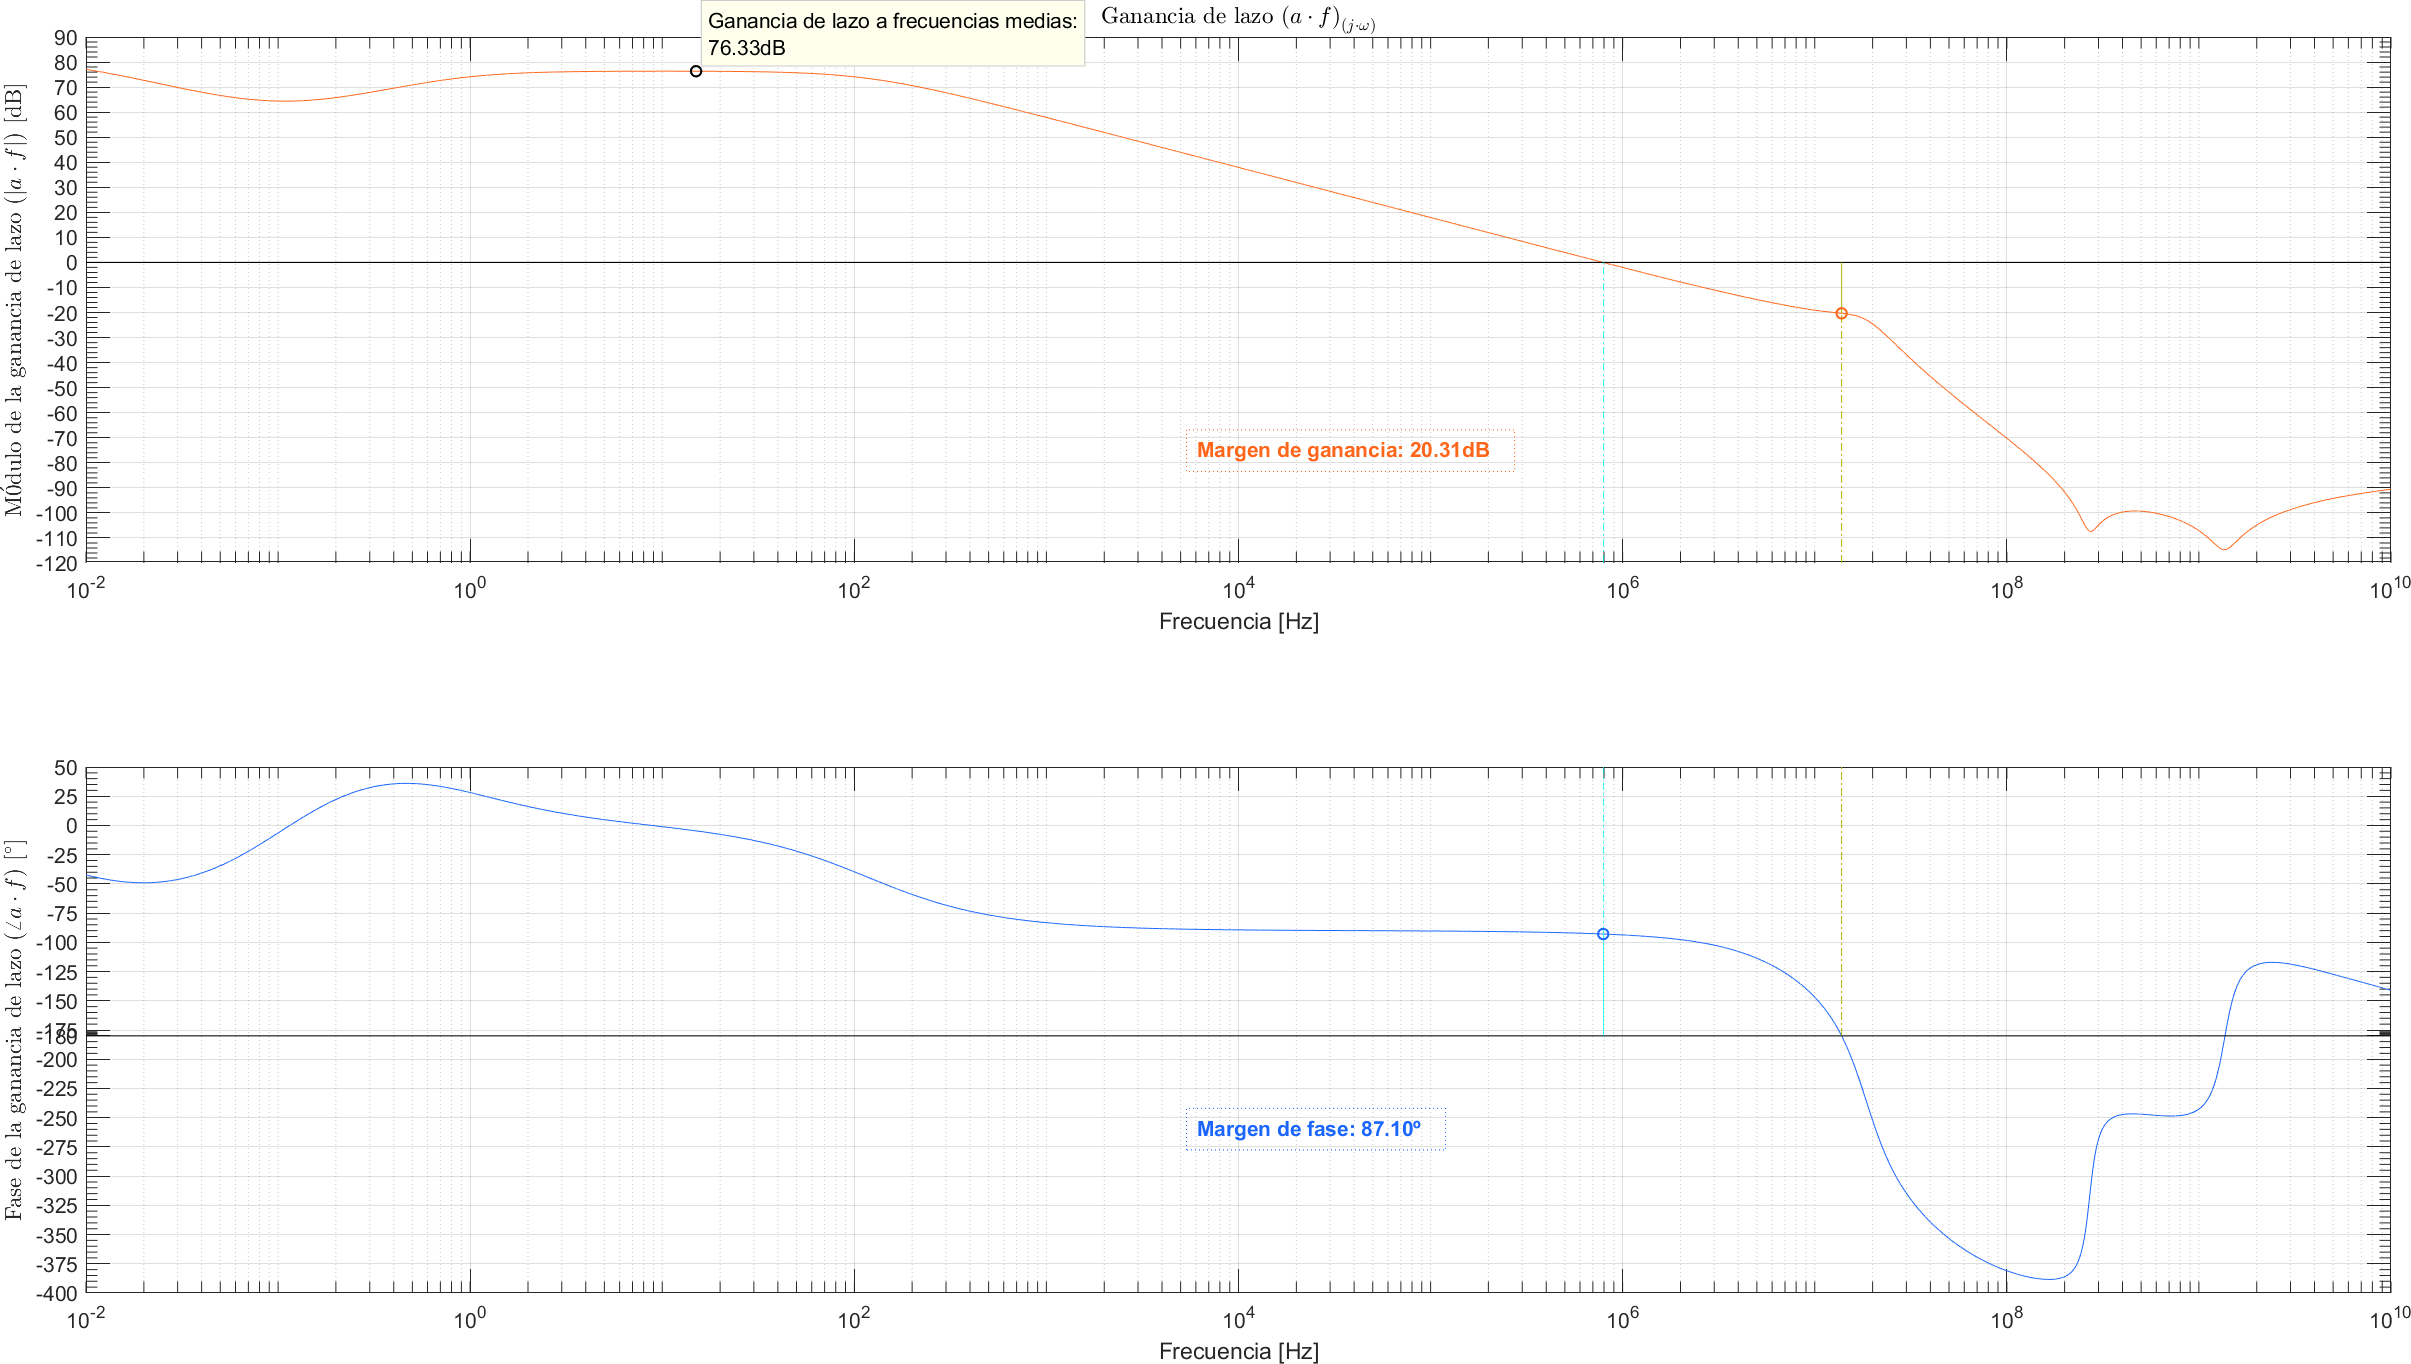
\includegraphics[width=0.85\paperwidth, angle=90]{img/sims/gain_loop_C.png}
	\caption{Bode de la ganancia de lazo compensado.}
	\label{fig:bode-la-con-comp}
\end{figure}

\clearpage


El margen de fase resultante ese de $87.1 \si[per-mode=symbol]{\degree}$ y el ancho de banda de $798 \si[per-mode=symbol]{\kilo\hertz}$, con un margen de ganancia de $20.3 \si[per-mode=symbol]{\decibel}$. Se puede ver en la figura~\figref{fig:slew} que la respuesta al escalón no oscila.

Se compensó el comportamiento inductivo del multiplicador de $V_{be}$ en altas frecuencias con el capacitor $CC_{2}$ de $6.8 \si[per-mode=symbol]{\nano\farad}$, su valor se halló simplemente aumentando el valor desde un valor de $1 \si[per-mode=symbol]{\nano\farad}$ hasta lograr una impedancia perfectamente plana en todo el ancho de banda, que luego cae monotonamente.

La última compensación, se trata de la compensación por alinealidad en la respuesta de los transistores de salida durante el switcheo, que puede verse claramente en las simulaciones, y es de alta frecuencia, esto se compensa colocando entre base y colector de los drivers externos los capacitores $CC_{3}$ y $CC_{4}$ de $68 \si[per-mode=symbol]{\pico\farad}$, valores hallados en forma empírica, y que probablemente requieran ajuste tras la medición del circuito armado.


Finalmente, con las ganancias a lazo abierto y lazo cerrado, realizamos el siguiente diagrama:

\begin{figure}[H]
	\centering
	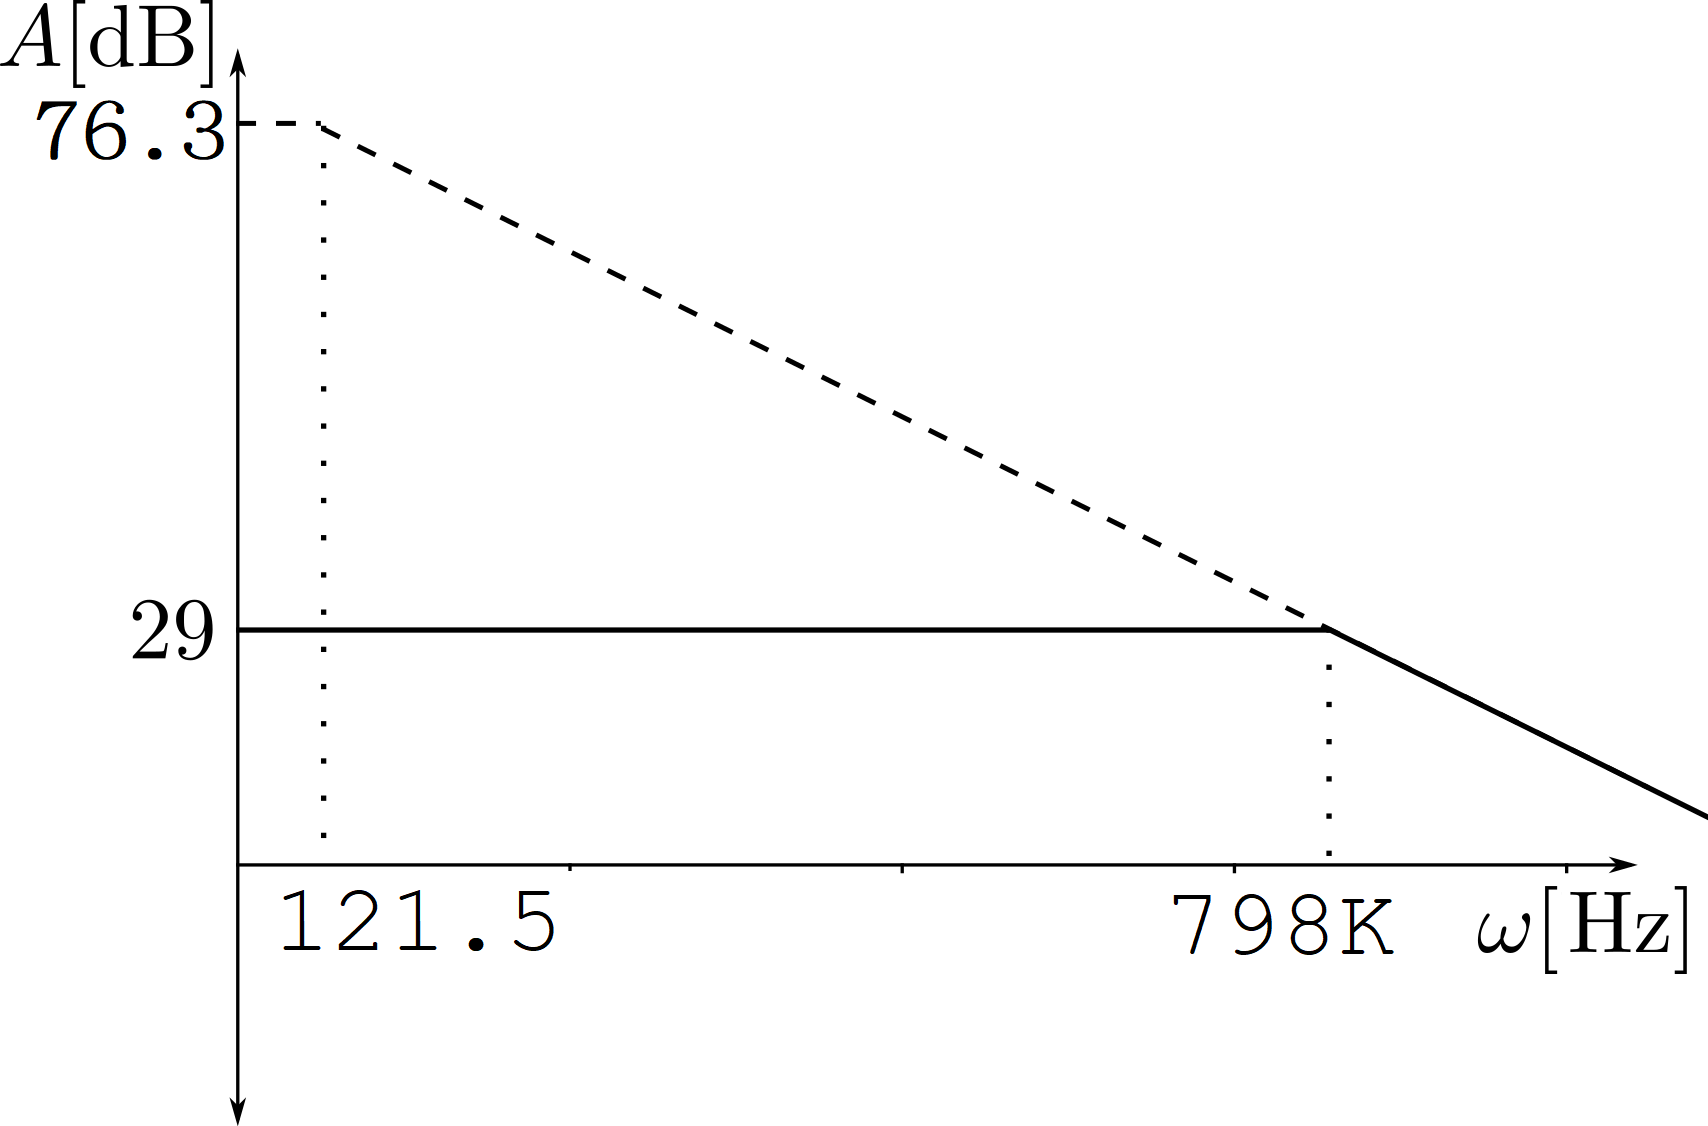
\includegraphics[width=0.5\textwidth]{img/bodecompensado.png}
	\caption{Aumento del ancho de banda, debido a la realimentación.}
	\label{fig:bode-compensado}
\end{figure}

Como se puede ver en el gráfico, la ganancia a lazo abierto, de $76.3 \si[per-mode=symbol]{\decibel}$, tiene un ancho de banda de $121.5 \si[per-mode=symbol]{\hertz}$, totalmente inútil para un amplificador de audio que trabaja con señales de decenas de $\si[per-mode=symbol]{\kilo\hertz}$. Cuando aplicamos la realimentación, la ganancia cae a $29 \si[per-mode=symbol]{\decibel}$, pero la frecuencia de corte pasa a ser $121.5 \si[per-mode=symbol]{\hertz} \times (1 + a_V \cdot f) = 122 \times 6569 = 798 \si[per-mode=symbol]{\kilo\hertz}$.
\clearpage
%\\\\\\\\\\\\\\\\\\\\\\\\\\\


%\\\\\\\\\\\\\\\\\\\\\\\\\\\
\section{Simulaciones}
\resetallcounters

\subsection{THD} 

A continuación se muestra una tabla con los resultados del análisis de Fourier realizados con el \textbf{LTSpice} con el comando \textbf{SPICE} \textit{\textbf{.four}} para entrada de $1.0795 \si[per-mode=symbol]{\volt}$ pico (máxima excursión, $60 \si[per-mode=symbol]{\watt}$) a $1 \si[per-mode=symbol]{\kilo\hertz}$. 


%******************************************************************************************
\lstset{language=,xleftmargin=1em,numbers=none}

\lstset{showspaces=false}
\lstset{showstringspaces=false}
\normalfont
\normalsize
\lstset{backgroundcolor=\color{white},rulecolor=\color{blue}}
\lstset{basicstyle=\ttfamily\color{red}}

\lstset{keywordstyle=[1]\ttfamily\color{red}\bfseries}
\lstset{keywordstyle=[2]\ttfamily\color{red}}
\lstset{keywordstyle=[3]\ttfamily\bfseries\color{red}}
\lstset{keywordstyle=[4]\ttfamily\bfseries\color{red}}

\lstset{identifierstyle=\ttfamily\color{red}}
\lstset{commentstyle=\ttfamily\color{red}\textit}
\lstset{stringstyle=\ttfamily\color{red}\upshape}
\lstset{tabsize=4}

\lstset{numberstyle=\ttfamily\color{red}\upshape}
\lstset{numbersep=5pt}

\lstset{extendedchars=\false, inputencoding=utf8x}



\fontencoding{T1}
\fontseries{m}
\fontsize{7pt}{8pt}
\selectfont
%******************************************************************************************

\begin{lstlisting}
N-Period=4
Fourier components of V(out)
DC component:-0.00609365

Harmonic	Frequency	 Fourier 	Normalized	 Phase  	Normalized
 Number 	  [Hz]   	Component	 Component	[degree]	Phase [deg]
    1   	1.000e+03	3.099e+01	1.000e+00	   -0.07	    0.00
    2   	2.000e+03	4.065e-04	1.312e-05	   78.76	   78.83
    3   	3.000e+03	7.184e-04	2.318e-05	    6.71	    6.78
    4   	4.000e+03	1.003e-04	3.235e-06	   93.85	   93.93
    5   	5.000e+03	4.902e-05	1.582e-06	  170.68	  170.75
    6   	6.000e+03	4.829e-05	1.558e-06	  -59.26	  -59.18
    7   	7.000e+03	1.293e-04	4.172e-06	   26.87	   26.94
    8   	8.000e+03	1.457e-05	4.702e-07	  104.20	  104.28
    9   	9.000e+03	4.272e-05	1.379e-06	   52.46	   52.54
   10   	1.000e+04	3.185e-05	1.028e-06	  -70.05	  -69.98
   11   	1.100e+04	4.199e-05	1.355e-06	   67.89	   67.96
   12   	1.200e+04	1.060e-05	3.420e-07	  -93.43	  -93.35
   13   	1.300e+04	3.133e-05	1.011e-06	  136.68	  136.75
   14   	1.400e+04	6.583e-06	2.124e-07	  -84.68	  -84.61
   15   	1.500e+04	3.250e-05	1.049e-06	  153.79	  153.87
   16   	1.600e+04	5.378e-06	1.735e-07	  112.21	  112.28
   17   	1.700e+04	2.309e-05	7.450e-07	  156.75	  156.83
   18   	1.800e+04	9.952e-06	3.211e-07	  100.07	  100.15
   19   	1.900e+04	9.865e-06	3.183e-07	  104.44	  104.51
   20   	2.000e+04	9.097e-06	2.935e-07	   94.78	   94.86
   21   	2.100e+04	1.826e-05	5.892e-07	   40.20	   40.28
   22   	2.200e+04	4.168e-06	1.345e-07	   80.56	   80.64
   23   	2.300e+04	2.337e-05	7.541e-07	   31.93	   32.01
   24   	2.400e+04	2.081e-06	6.716e-08	  -37.14	  -37.07
   25   	2.500e+04	1.654e-05	5.337e-07	   33.14	   33.21
   26   	2.600e+04	4.155e-06	1.341e-07	  -67.28	  -67.21
   27   	2.700e+04	2.669e-06	8.613e-08	   61.95	   62.02
   28   	2.800e+04	2.670e-06	8.615e-08	  -78.19	  -78.12
   29   	2.900e+04	1.103e-05	3.558e-07	 -154.32	 -154.25
   30   	3.000e+04	1.358e-06	4.381e-08	  133.87	  133.94
Total Harmonic Distortion: 0.002742%(0.002742%)

\end{lstlisting}

\normalfont
\normalsize


La distorsión armónica simulada es de $0.0027 \si[per-mode=symbol]{\percent}$ en la máxima excursión a $1 \si[per-mode=symbol]{\kilo\hertz}$. El resultado para una simulación similar a $10 \si[per-mode=symbol]{\kilo\hertz}$ se muestra a continuación:



\clearpage



%******************************************************************************************
\fontencoding{T1}
\fontseries{m}
\fontsize{7pt}{8pt}
\selectfont
%******************************************************************************************


\begin{lstlisting}
N-Period=4
Fourier components of V(out)
DC component:-0.000245223

Harmonic	Frequency	 Fourier 	Normalized	 Phase  	Normalized
 Number 	  [Hz]   	Component	 Component	[degree]	Phase [deg]
    1   	1.000e+04	3.099e+01	1.000e+00	   -0.86	    0.00
    2   	2.000e+04	1.108e-03	3.575e-05	  -55.41	  -54.55
    3   	3.000e+04	8.353e-04	2.695e-05	   29.81	   30.67
    4   	4.000e+04	7.803e-04	2.518e-05	 -104.83	 -103.97
    5   	5.000e+04	1.439e-04	4.644e-06	 -166.50	 -165.64
    6   	6.000e+04	7.527e-04	2.429e-05	  -81.99	  -81.13
    7   	7.000e+04	3.855e-04	1.244e-05	   78.77	   79.62
    8   	8.000e+04	4.484e-04	1.447e-05	 -108.78	 -107.92
    9   	9.000e+04	9.610e-05	3.101e-06	  123.98	  124.84
   10   	1.000e+05	3.037e-04	9.801e-06	  -83.93	  -83.08
   11   	1.100e+05	8.219e-05	2.652e-06	   78.36	   79.22
   12   	1.200e+05	8.684e-05	2.802e-06	 -108.53	 -107.67
   13   	1.300e+05	1.085e-04	3.501e-06	  -84.14	  -83.29
   14   	1.400e+05	1.247e-05	4.025e-07	   51.25	   52.11
   15   	1.500e+05	1.942e-04	6.267e-06	  -76.55	  -75.70
   16   	1.600e+05	5.183e-05	1.672e-06	  120.09	  120.95
   17   	1.700e+05	2.269e-04	7.322e-06	  -81.74	  -80.89
   18   	1.800e+05	6.231e-05	2.011e-06	  175.95	  176.80
   19   	1.900e+05	1.662e-04	5.363e-06	  -93.66	  -92.81
   20   	2.000e+05	1.084e-04	3.497e-06	 -148.53	 -147.67
   21   	2.100e+05	8.073e-05	2.605e-06	 -146.75	 -145.89
   22   	2.200e+05	1.279e-04	4.126e-06	 -133.60	 -132.74
   23   	2.300e+05	1.299e-04	4.191e-06	  140.65	  141.51
   24   	2.400e+05	8.677e-05	2.800e-06	 -118.21	 -117.35
   25   	2.500e+05	1.712e-04	5.526e-06	  120.85	  121.70
   26   	2.600e+05	3.611e-05	1.165e-06	  -30.78	  -29.93
   27   	2.700e+05	1.205e-04	3.889e-06	  108.09	  108.95
   28   	2.800e+05	9.993e-05	3.225e-06	   27.09	   27.94
   29   	2.900e+05	1.951e-05	6.297e-07	   16.45	   17.31
   30   	3.000e+05	1.251e-04	4.037e-06	   39.61	   40.47
Total Harmonic Distortion: 0.006334%(0.010095%)

\end{lstlisting}

\normalfont
\normalsize


La distorsión total es de $0.006 \si[per-mode=symbol]{\percent}$. Haciendo simulaciones similares se obtiene que para $1 \si[per-mode=symbol]{\watt}$ ($4 \si[per-mode=symbol]{\volt}$) de salida, y $1 \si[per-mode=symbol]{\kilo\hertz}$, la distorsión es de $0.000217 \si[per-mode=symbol]{\percent}$ y a $10 \si[per-mode=symbol]{\kilo\hertz}$, $0.002 \si[per-mode=symbol]{\percent}$. En todos los casos se cumple lo especificado.




En la figura~\figref{fig:distorsion-barrido-1} se muestra la distorsión a $1 \si[per-mode=symbol]{\kilo\hertz}$ en función de la potencia de salida y en la figura~\figref{fig:distorsion-barrido-2} lo mismo, pero a $10 \si[per-mode=symbol]{\kilo\hertz}$.

\clearpage


\begin{figure}[H]
	\centering
	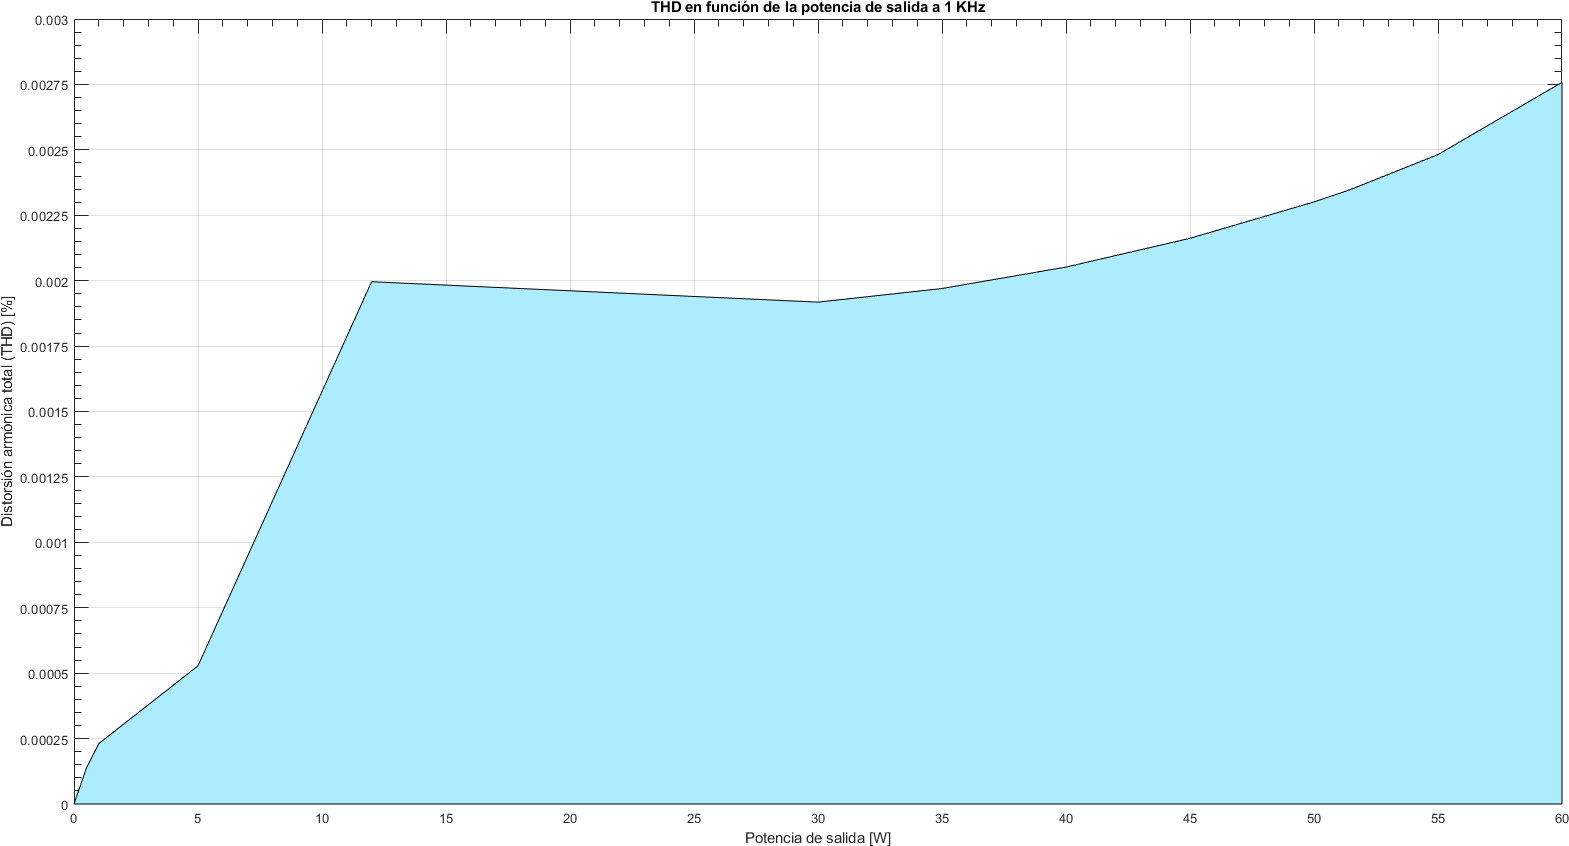
\includegraphics[width=0.7\paperheight, angle=90]{img/sims/distorsion-barrido-1.png}
	\caption{Distorsión a $1 \si[per-mode=symbol]{\kilo\hertz}$ a distintos valores de potencia de salida.}
	\label{fig:distorsion-barrido-1}
\end{figure}

\clearpage


\begin{figure}[H]
	\centering
	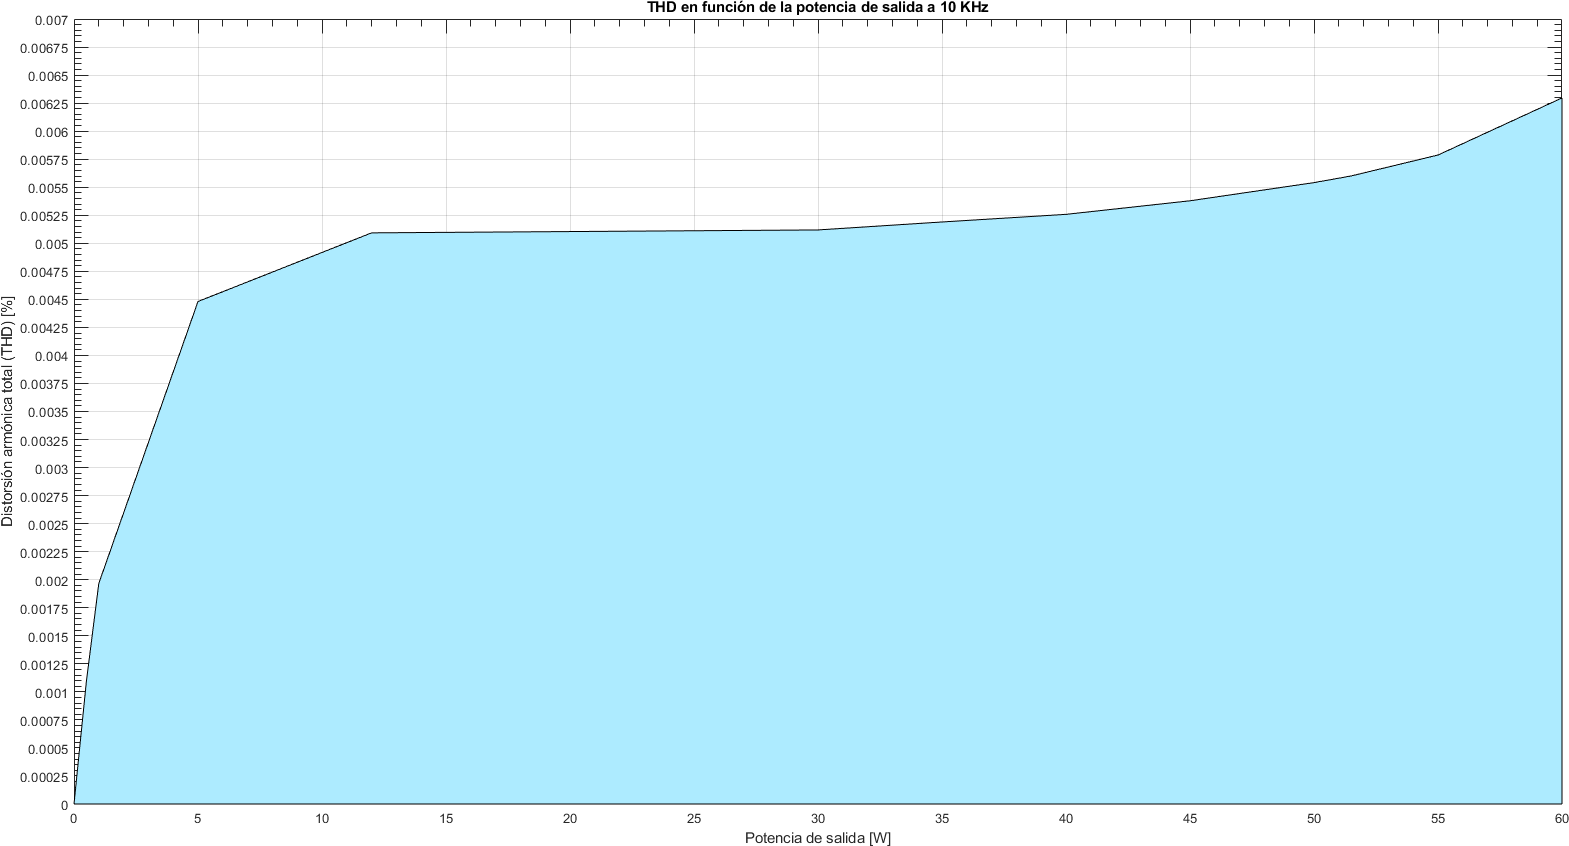
\includegraphics[width=0.7\paperheight, angle=90]{img/sims/distorsion-barrido-2.png}
	\caption{Distorsión a $10 \si[per-mode=symbol]{\kilo\hertz}$ a distintos valores de potencia de salida.}
	\label{fig:distorsion-barrido-2}
\end{figure}

\clearpage

\begin{figure}[H]
	\centering
	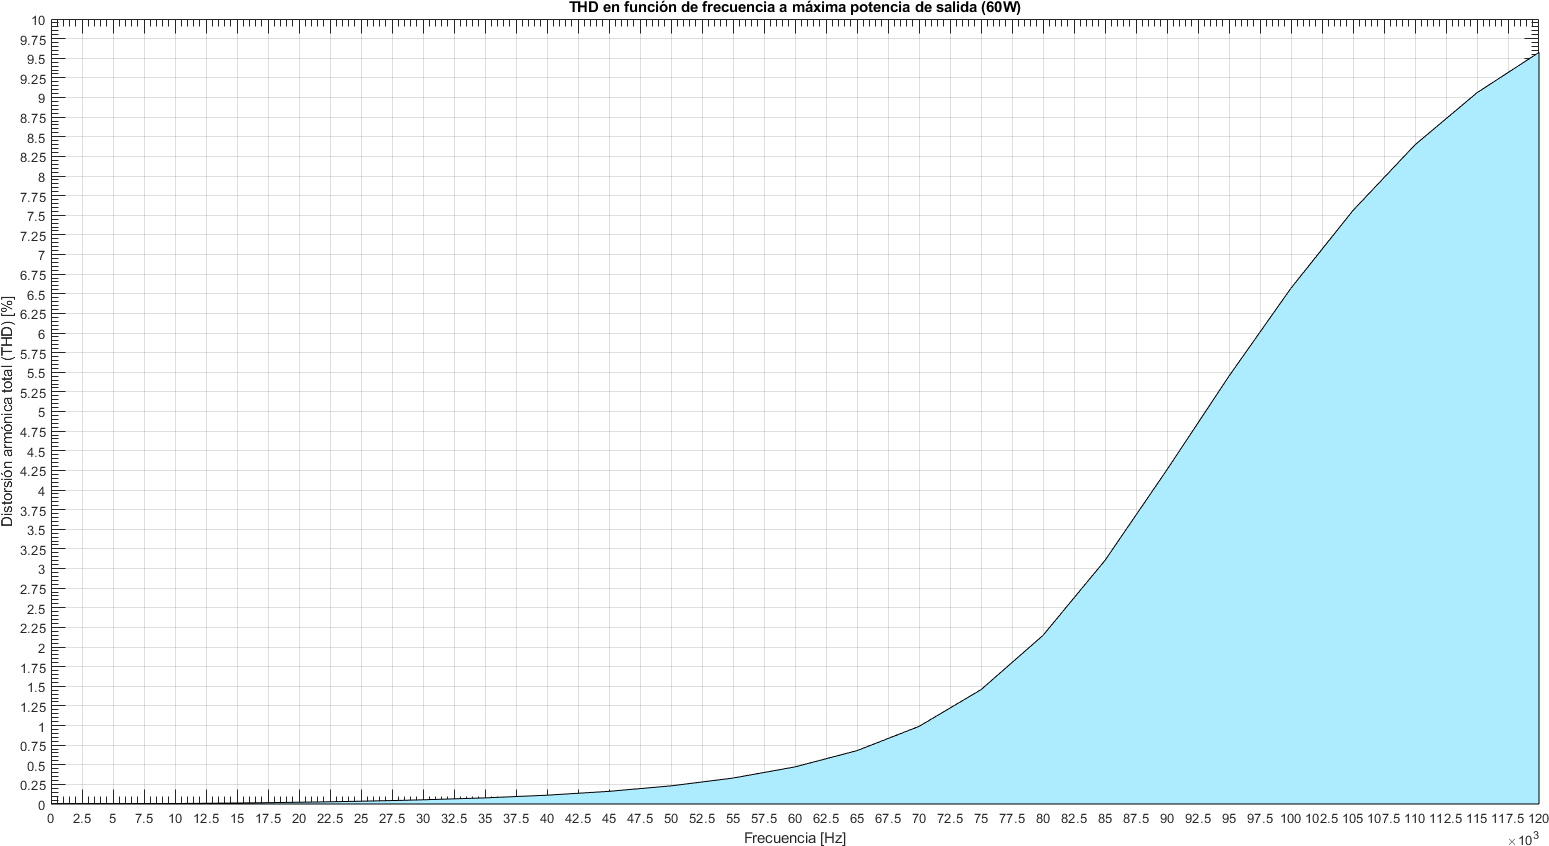
\includegraphics[width=0.7\paperheight, angle=90]{img/sims/distorsion-frec.png}
	\caption{Distorsión a máxima excursión en función de la frecuencia.}
	\label{fig:distorsion-frec}
\end{figure}

\clearpage



Los valores de distorsión bajan a potencias menores porque se reduce la distorsión por alinealidad de los transistores: mientras más chica es la excursión, más uno se encuentra en pequeña señal, y más lineal es la relación entre $v_{be}$ e $i_{c}$. Por otra parte, se colocó al multiplicador de $V_{be}$ de modo tal que haga funcionar a la etapa de salida en modo A-B, reduciendo la distorsión por crossover, de todos modos se puede observar como a partir de alrededor $12 \si[per-mode=symbol]{\watt}$, que corresponde a una tensión de alrededor de $14 \si[per-mode=symbol]{\volt}$, tensión a la cual se empieza a producir el sewitcheo de los transistores externos, la distorsión deja de crecer linealmente por pasar a estar dominada por la distorsión de switching en lugar de la de crossover.

La figura~\figref{fig:distorsion-frec}, por su parte, muestra resultados de simulaciones de distorsión a máxima excursión en función de la frecuencia, puede verse como alrededor de los $80 \si[per-mode=symbol]{\kilo\hertz}$ crece mas abruptamente la distorsión, esto se justifica en la próxima sección con el Slew-Rate del circuito, puede verse como la distorsión crece acercándose al $12 \si[per-mode=symbol]{\percent}$ que corresponde a una triangular.



\subsection{Slew Rate} Simulando una entrada escalón en el amplificador, se observa la salida de la figura~\figref{fig:slew_zoom} en la carga.

La pendiente es de $19.3 \si[per-mode=symbol]{\volt\per\micro\second}$. Esto es mayor a la máxima pendiente de la salida en máxima potencia a la máxima frecuencia especificada de $30 \si[per-mode=symbol]{\kilo\hertz}$, por lo que el ancho de banda de potencia cumplirá lo especificado ($15 \si[per-mode=symbol]{\volt\per\micro\second} < 19.3 \si[per-mode=symbol]{\volt\per\micro\second} $).

Para hallar el SR de manera teórica, partimos de la fuente de corriente de un par diferencial. La corriente que generan es de $3.15 \si[per-mode=symbol]{\milli\ampere}$, es decir, $1.57 \si[per-mode=symbol]{\milli\ampere}$ por rama. Si dividimos este valor por el capacitor de Miller ($100 \si[per-mode=symbol]{\pico\farad}$), nos queda un SR de $15.7 \si[per-mode=symbol]{\volt\per\micro\second}$. Si calculamos el ancho de banda de potencia, con este \textbf{SR}, nos da que la frecuencia máxima a la que el amplificador puede desarrollar $31 \si[per-mode=symbol]{\volt}$ pico, de salida, es $80.6 \si[per-mode=symbol]{\kilo\hertz}$. A pesar de que el \textbf{SR} nos dio menos que en la simulación, el ancho de banda sigue cumpliendo con las especificaciones. Esta diferencia se debe a que la simulación utiliza un método numérico para hallar las respuestas con un error pequeño, y el cálculo teórico se basa en varias hipótesis para simplificar el cálculo. Será importante, a la hora de armar el circuito, que éste funcione dentro de los parámetros esperados.

\clearpage

\begin{figure}[H]
	\centering
	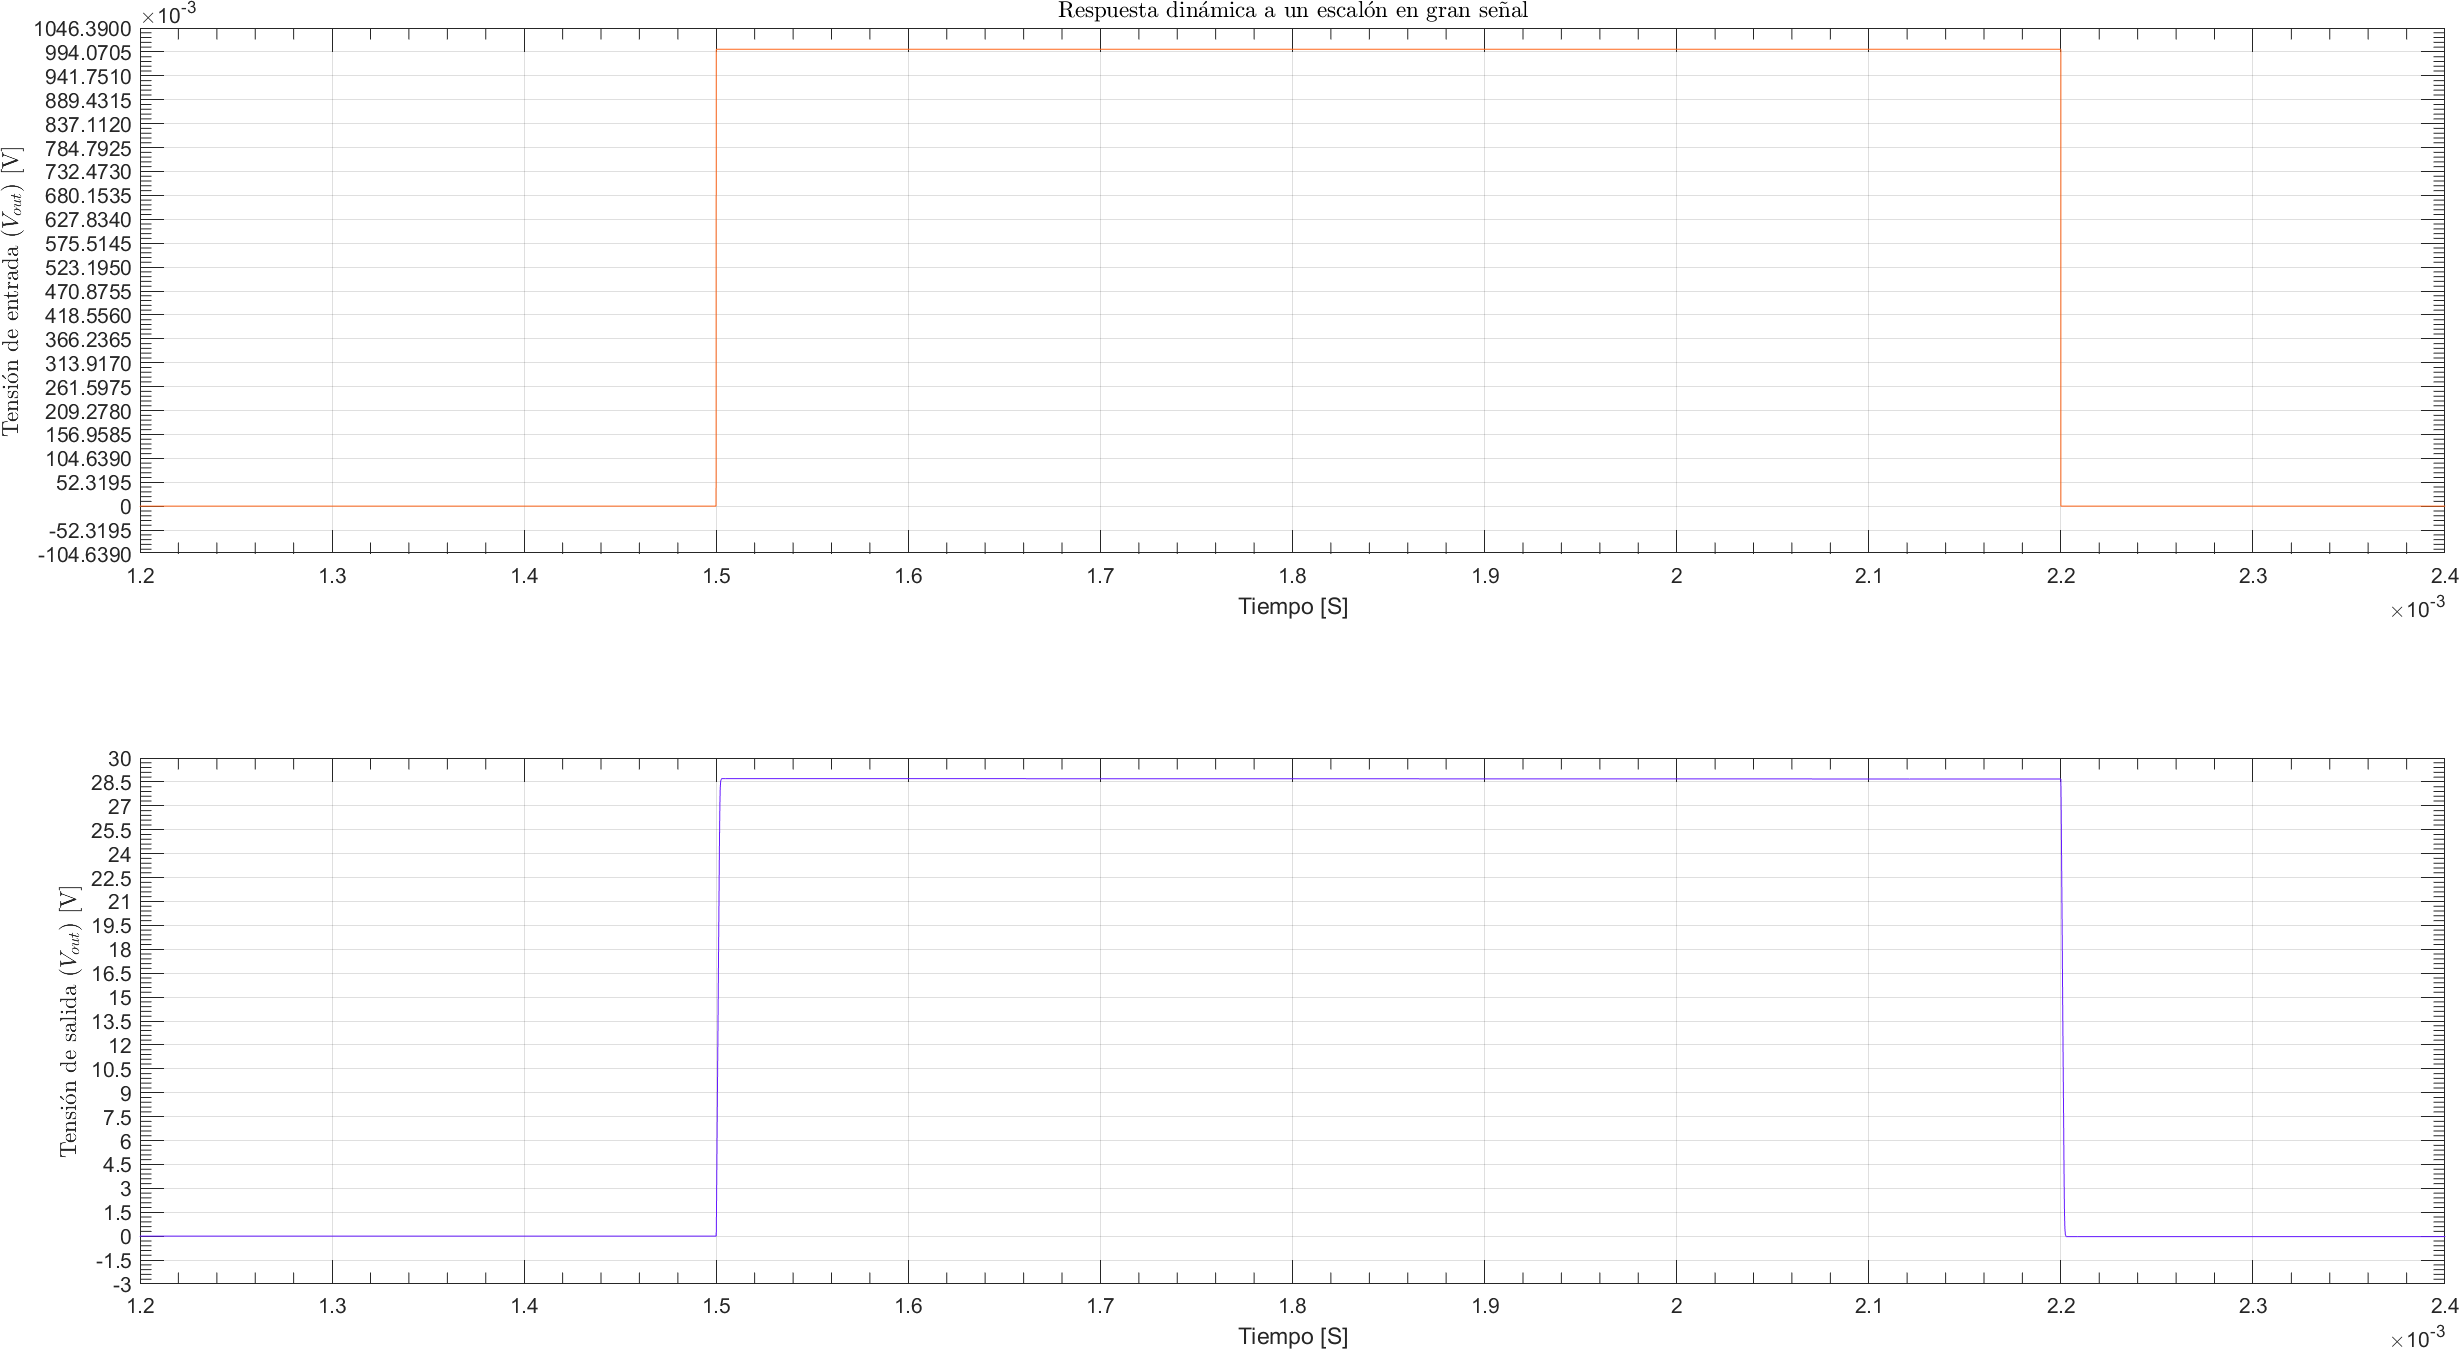
\includegraphics[width=0.7\paperheight, angle=90]{img/sims/Slew_Rate.png}
	\caption{Respuesta frente a una entrada escalón.}
	\label{fig:slew}
\end{figure}

\clearpage

\begin{figure}[H]
	\centering
	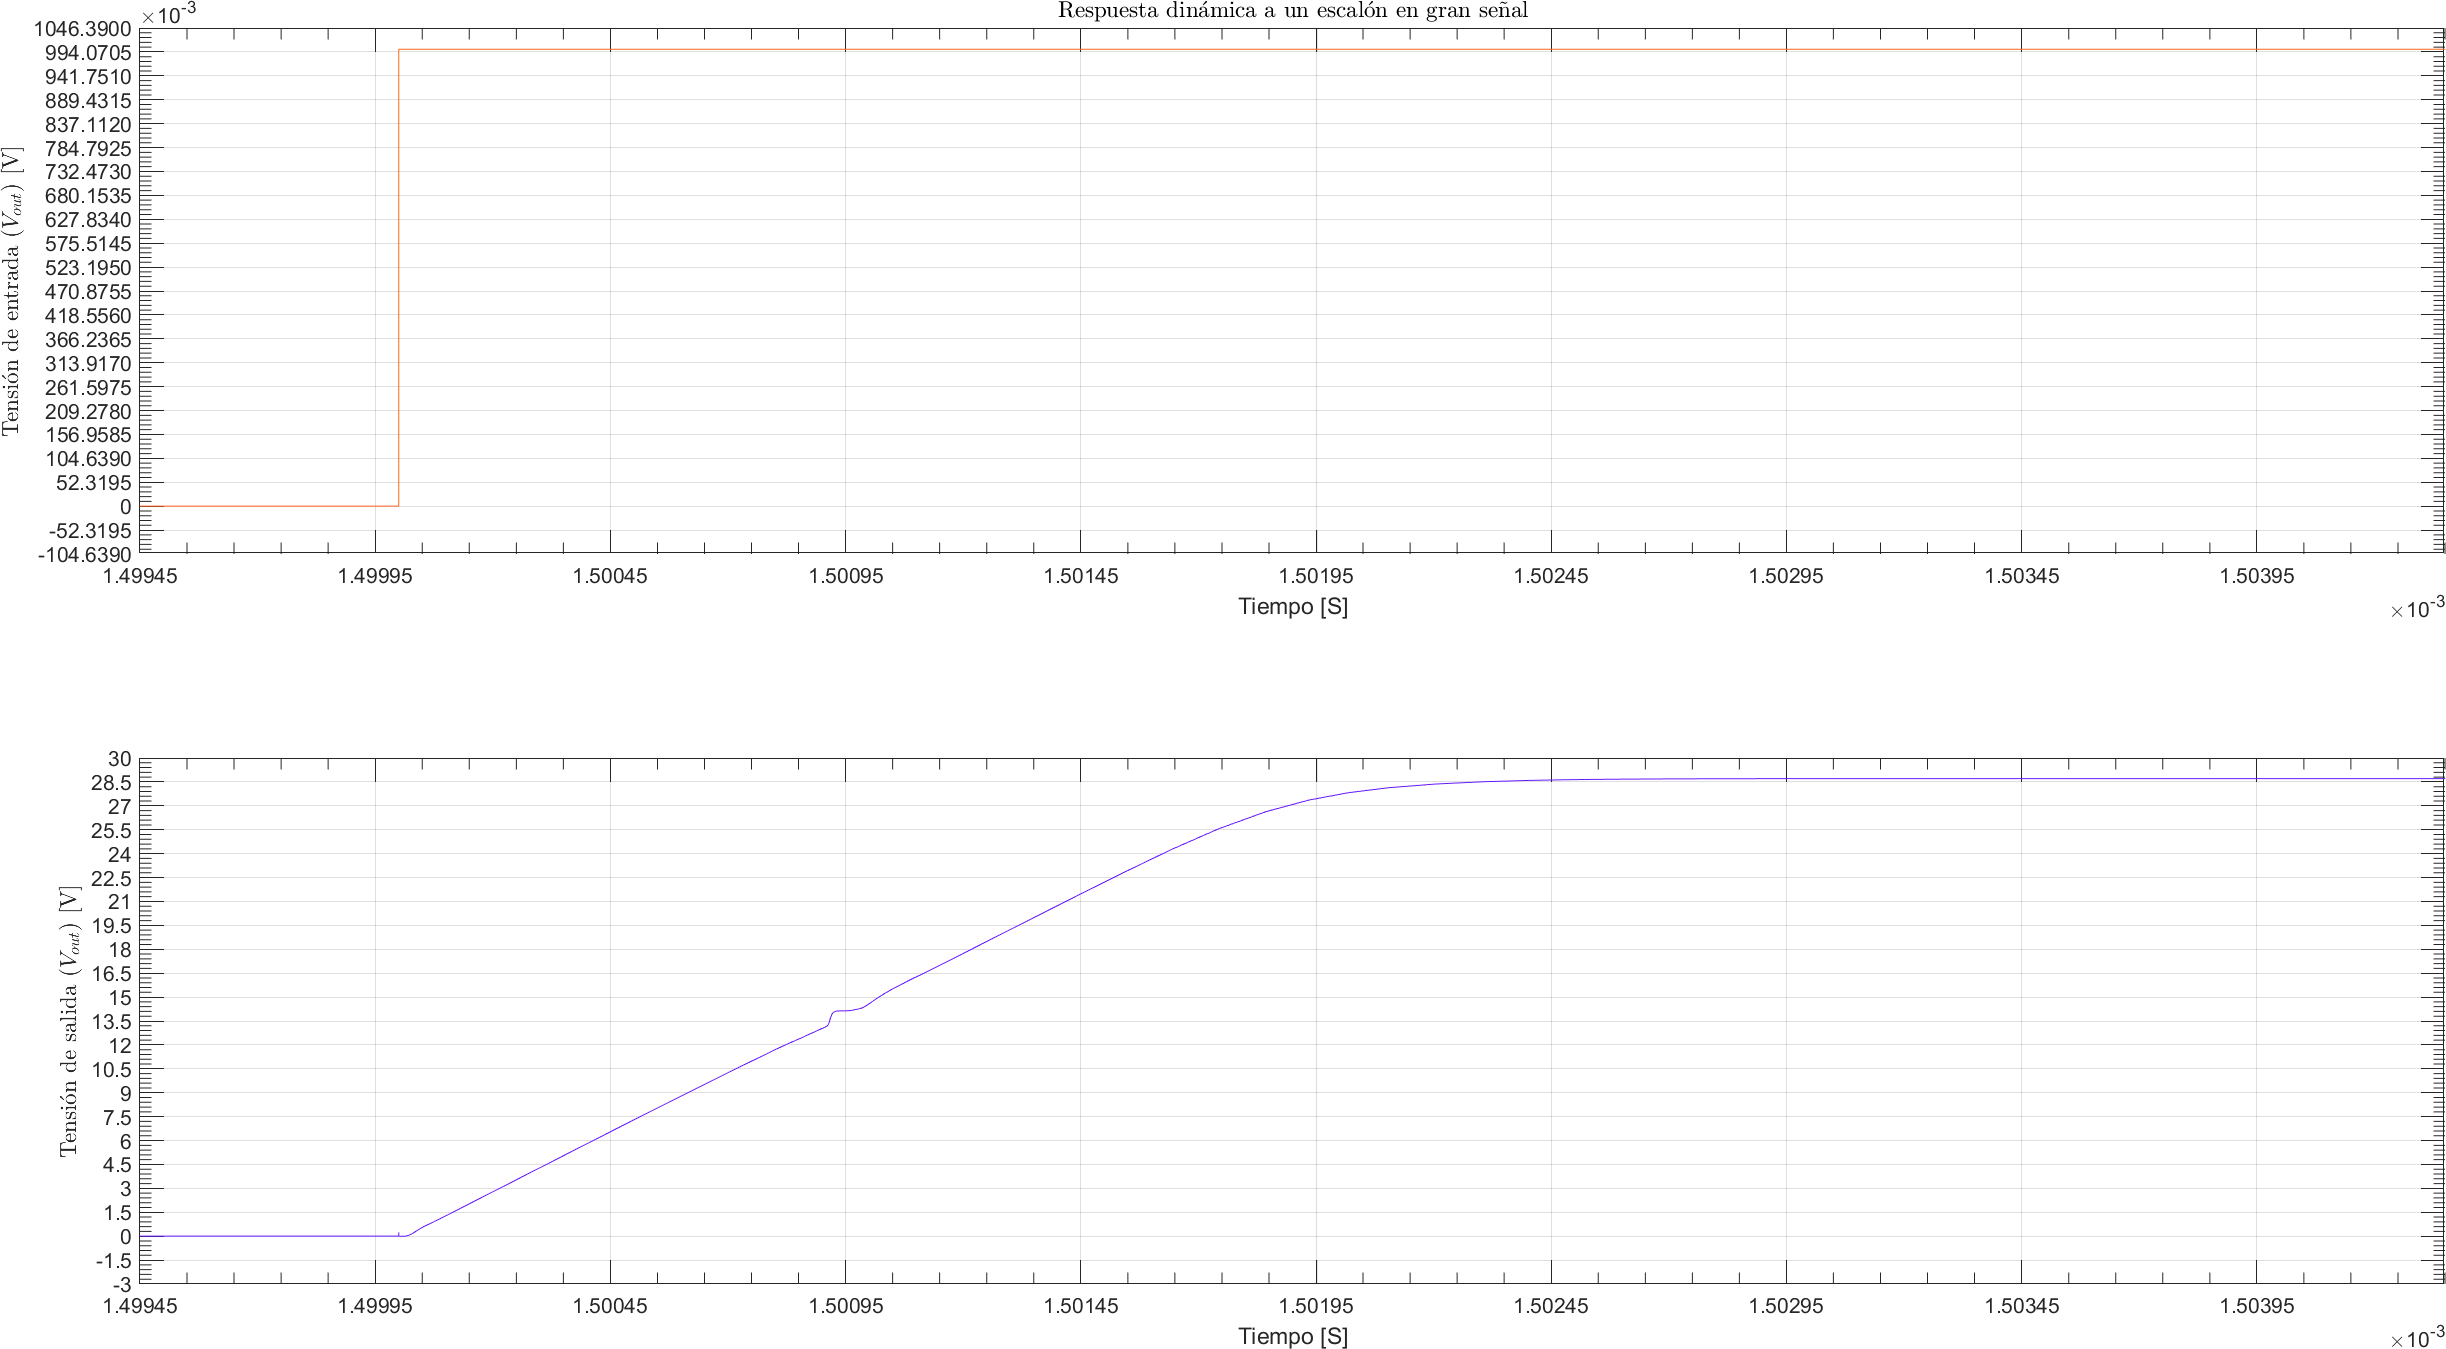
\includegraphics[width=0.7\paperheight, angle=90]{img/sims/Slew_Rate_Zoom.png}
	\caption{Respuesta frente a una entrada escalón, zoom sobre la pendiente.}
	\label{fig:slew_zoom}
\end{figure}

\clearpage

\subsection{CMRR - factor de rechazo de modo común}

Un amplificador diferencial ideal debería amplificar, como dice su nombre, las diferencias entre las tensiones de entrada, e ignorar la tensión media. El parámetro \textbf{CMRR} mide cuan bien esto se logra, como el cociente entre la ganancia de modo común $A_{c}$ y la de modo diferencial $A_{d}$. 

\subsubsection{Modo común} 

Se simuló la primera etapa frente una entrada común de $100 \si[per-mode=symbol]{\milli\volt}$ con el circuito de la figura~\figref{fig:ac} y se obtuvo la ganancia de modo común. Para cada par diferencial del doble par, cuyas salidas son $o_{1}$ y $o_{2}$ en la figura~\figref{fig:ac}, se obtuvieron $A_{d}^{NPN}=\frac{V_{o_{1}}}{100 \si[per-mode=symbol]{\milli\volt}}$ y $A_{d}^{PNP}=\frac{V_{o_{2}}}{100 \si[per-mode=symbol]{\milli\volt}}$ como la relación entre la salida (pico) correspondiente al par y la entrada común (pico). 


\begin{figure}[H]
	\centering
	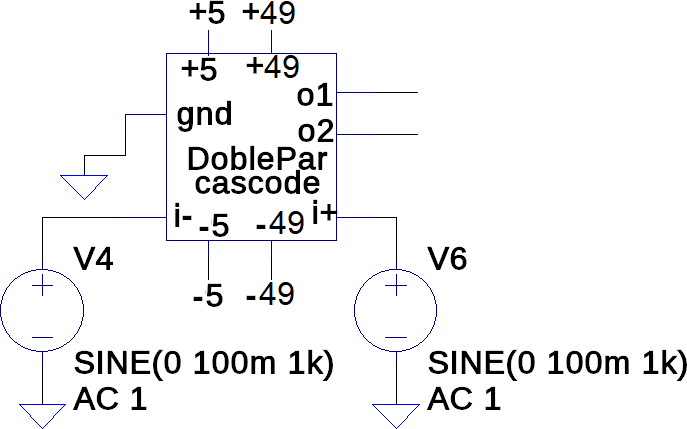
\includegraphics[height=0.2\textwidth]{img/sims/ac.png}
	\caption{Circuito usado para simular la amplificación de modo común.}
	\label{fig:ac}
\end{figure}

\subsubsection{Modo diferencial}

La amplificación de modo diferencial se obtuvo de forma análoga, con las fuentes de la figura~\figref{fig:ac} conectadas a contrafase. Las tensiones pico de las fuentes usadas fueron de sólo $1 \si[per-mode=symbol]{\milli\volt}$ porque se esperaba una amplificación mucho mayor que para el caso de modo común. Es decir, $A_{d}^{NPN}=\frac{V_{o_{1}}}{2 \si[per-mode=symbol]{\milli\volt}}$, y $A_{d}^{PNP}=\frac{V_{o_{2}}}{2 \si[per-mode=symbol]{\milli\volt}}$.

\subsubsection{CMRR} 

El factor de rechazo es simplemente $\frac{A_{d}}{A_{c}}$, en valor absoluto.


\begin{table}[H]
\centering
\begin{tabular}{l|ll}
 & NPN & PNP \\ \hline
$A_{c}$ & $-36.23 \si[per-mode=symbol]{\decibel}$ & $-41.32 \si[per-mode=symbol]{\decibel}$  \\
$A_{d}$ & $35.37 \si[per-mode=symbol]{\decibel}$ & $36.49 \si[per-mode=symbol]{\decibel}$  \\
RRMC & $71.6 \si[per-mode=symbol]{\decibel}$ & $77.81 \si[per-mode=symbol]{\decibel}$  
\end{tabular}
\end{table}

\clearpage

\subsection{\textbf{PSRR} - factor de rechazo del ripple la fuente}

El \textbf{PSRR} se define como la relación entre el cambio en la tensión de alimentación y el cambio equivalente en la tensión de entrada. Idealmente este valor sería infinito.

Simulando utilizando una fuente en forma de rampa invertida de $100 \si[per-mode=symbol]{\hertz}$ en serie con las fuentes de alimentación, pasivando la fuente de entrada y midiendo la amplitud de la señal de $100 \si[per-mode=symbol]{\hertz}$ y sus armónicos resultantes a la salida se obtuvo:

\[ PSRR := {\Delta V_\mathrm{fuente} \over {\Delta V_\mathrm{o}}} \cdot A_d = 111.3 \si[per-mode=symbol]{\decibel} \]



Es decir, con la ganancia de $29 \si[per-mode=symbol]{\decibel}$ de este circuito, por cada $1 \si[per-mode=symbol]{\volt}$ de ripple en la fuente de $+49 \si[per-mode=symbol]{\volt}$ se superponen aproximadamente $76.74 \si[per-mode=symbol]{\micro\volt}$ en la salida ($111.3 \si[per-mode=symbol]{\decibel} - 29 \si[per-mode=symbol]{\decibel} = 82.3 \si[per-mode=symbol]{\decibel}$ y $10^\frac{-82.3}{20} \cong 76.74 \si[per-mode=symbol]{\micro\volt} $)

También, se simuló y verificó el comportamiento correcto del amplificador para una posible caída de tensión en los rieles del $20 \si[per-mode=symbol]{\percent}$: sólo se reduce la máxima excursión, de donde se tomó la máxima excursión de $31 \si[per-mode=symbol]{\volt}$ en esta, la peor condición.

En nuestro caso, al utilizarse una fuente de alimentación no regulada, es realmente importante el rechazo de ripple de la fuente, ya que este es del orden de $2.5 \si[per-mode=symbol]{\volt}$ de pico cuando el amplificador está funcionando a máxima potencia, según lo simulado.

\subsection{Resistencia de salida}  

Para la simulación de la resistencia de salida, se colocó una fuente de corriente alterna de $1 \si[per-mode=symbol]{\ampere}$ a la salida, con la entrada pasivada, y se capturó la tensión de salida en un barrido de frecuencias.


El circuito simulado, con una caja representando el amplificador, se observa en la figura~\figref{fig:circuito_r-out-current}.


\begin{figure}[H]
	\centering
	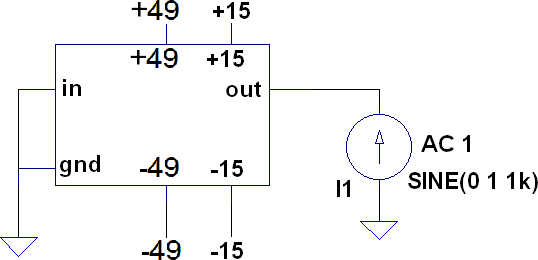
\includegraphics[width=0.6\textwidth]{img/sims/circuito-r_out-current.png}
	\caption{Circuito usado para simular la resistencia de salida. La caja representa al amplificador.}
	\label{fig:circuito_r-out-current}
\end{figure}

Los resultados del barrido se muestran en la figura~\figref{fig:R_out}, y un zoom en las frecuencias de trabajo especificadas en la figura~\figref{fig:R_out-zoom}.

\begin{figure}[H]
	\centering
	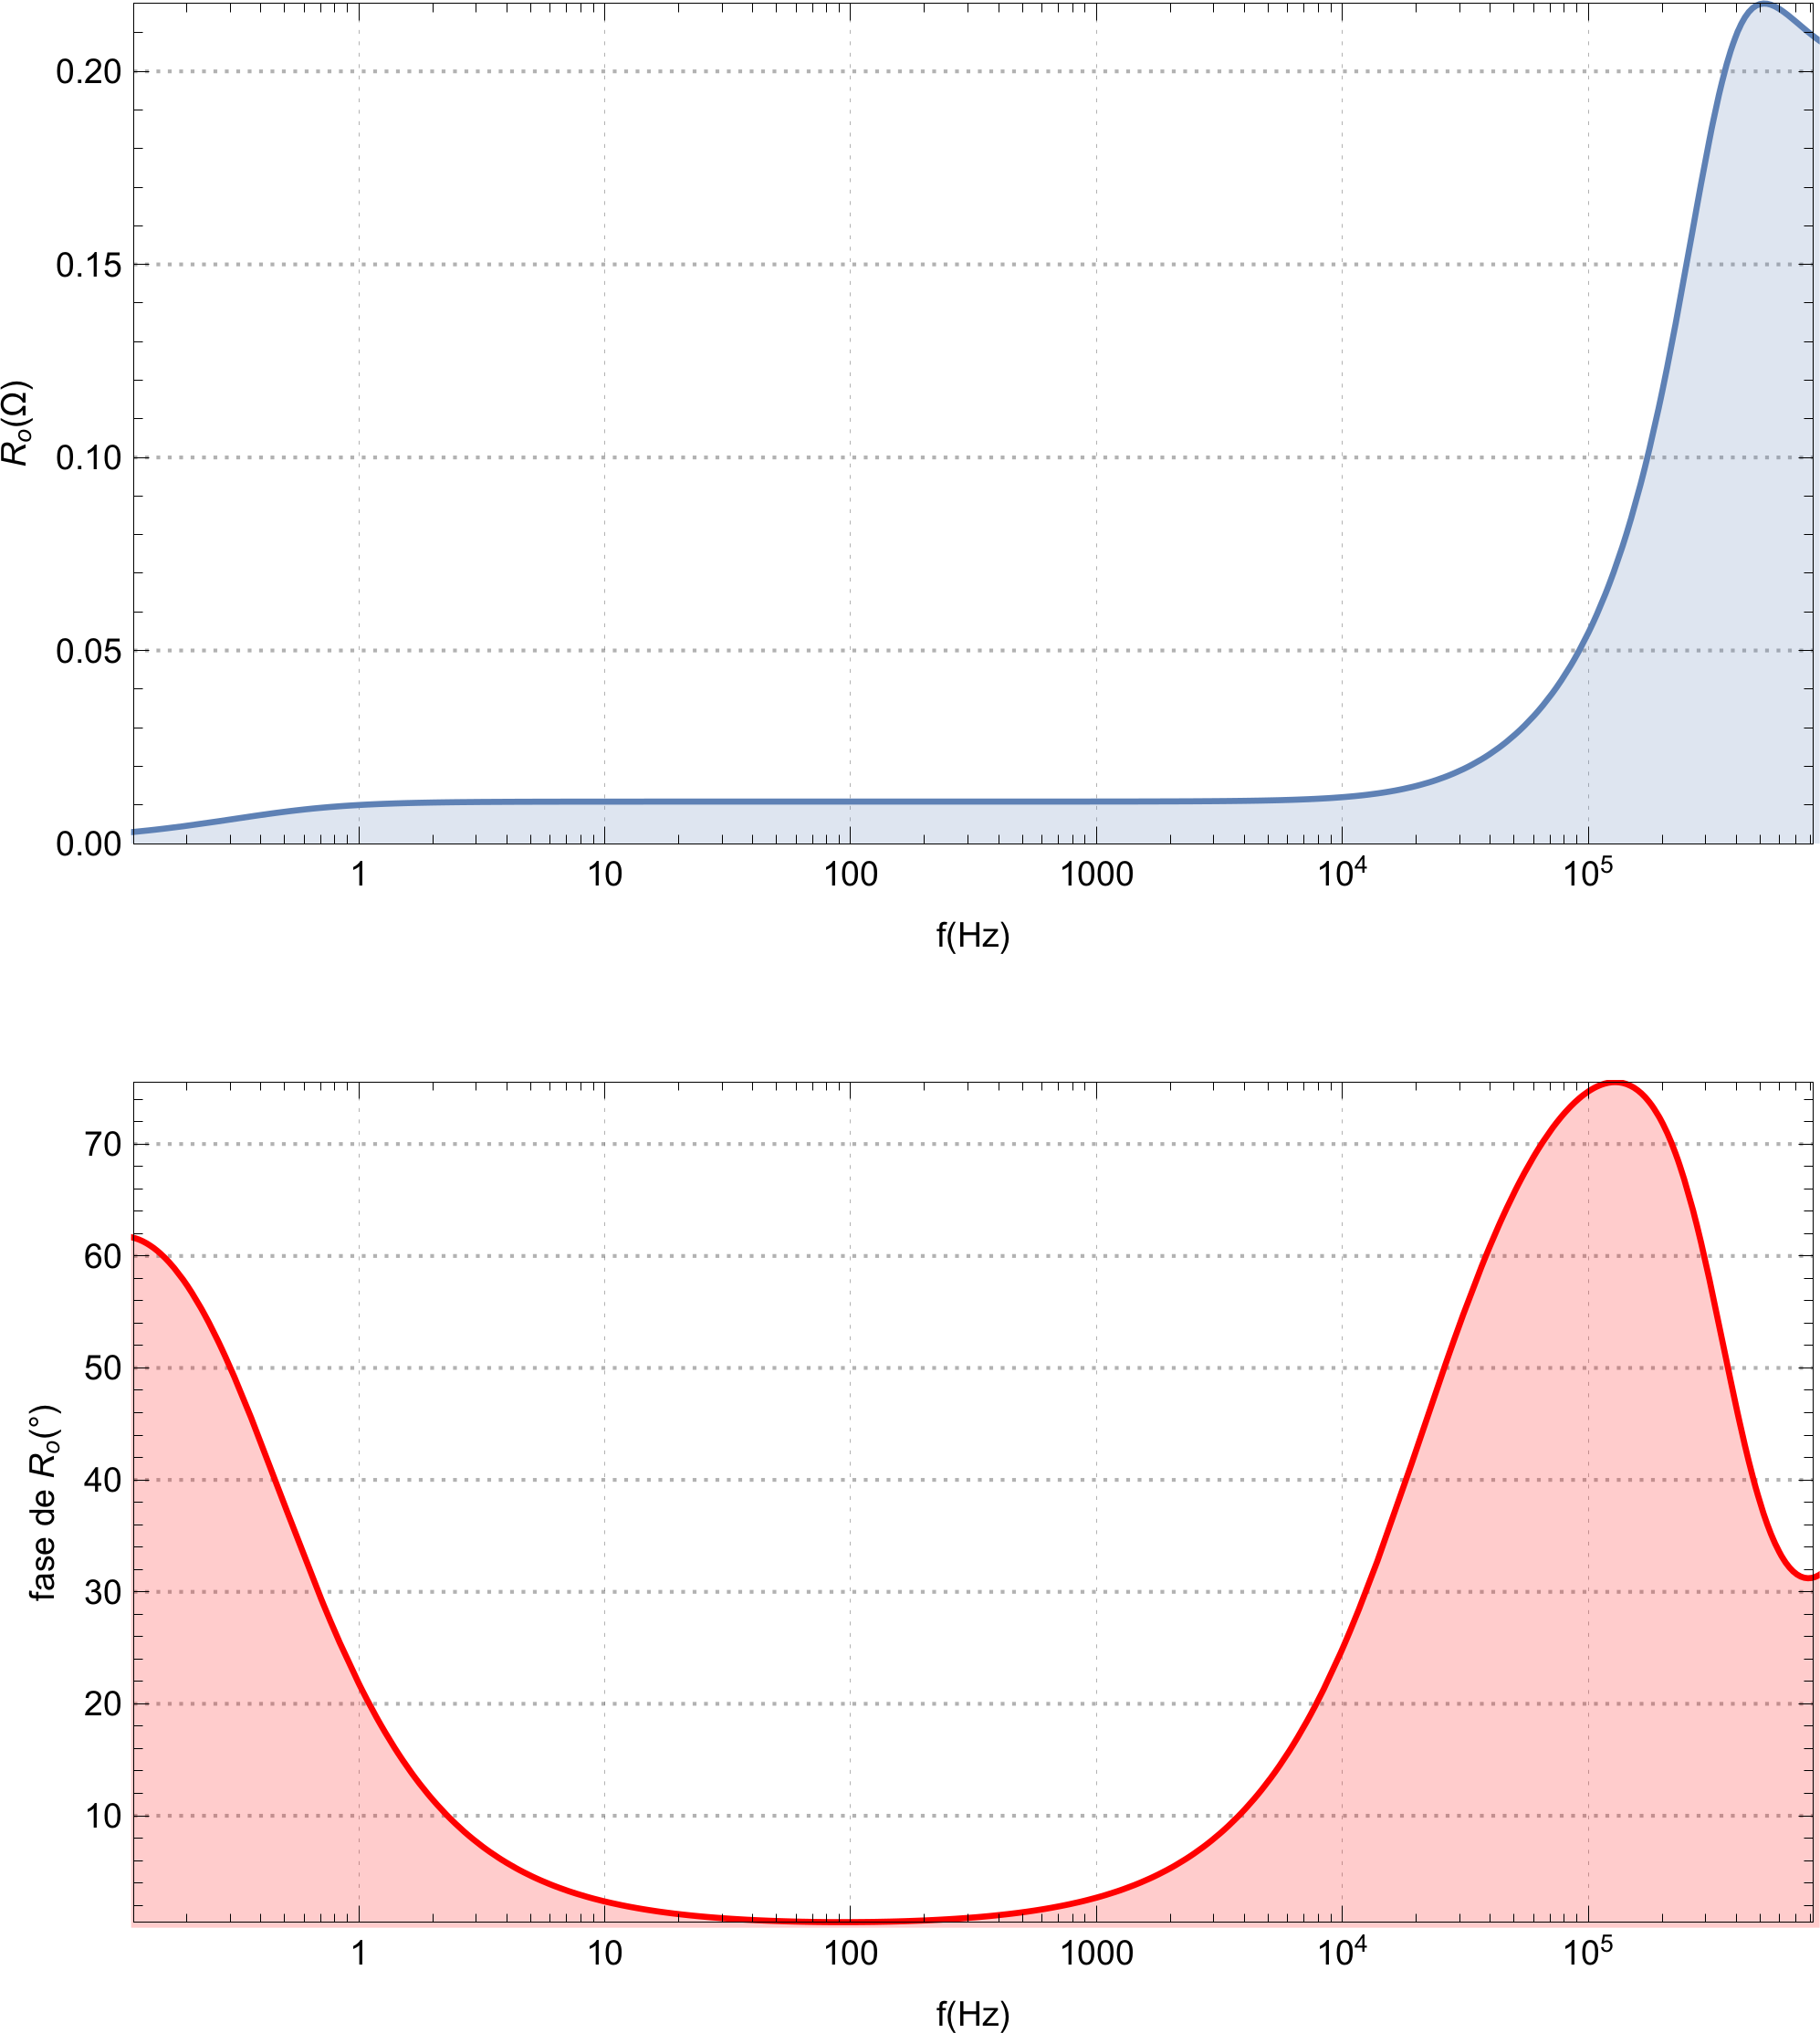
\includegraphics[width=0.8\textwidth]{img/sims/R_out.png}
	\caption{Barrido en frecuencias de la impedancia de salida simulada.}
	\label{fig:R_out}
\end{figure}

\begin{figure}[H]
	\centering
	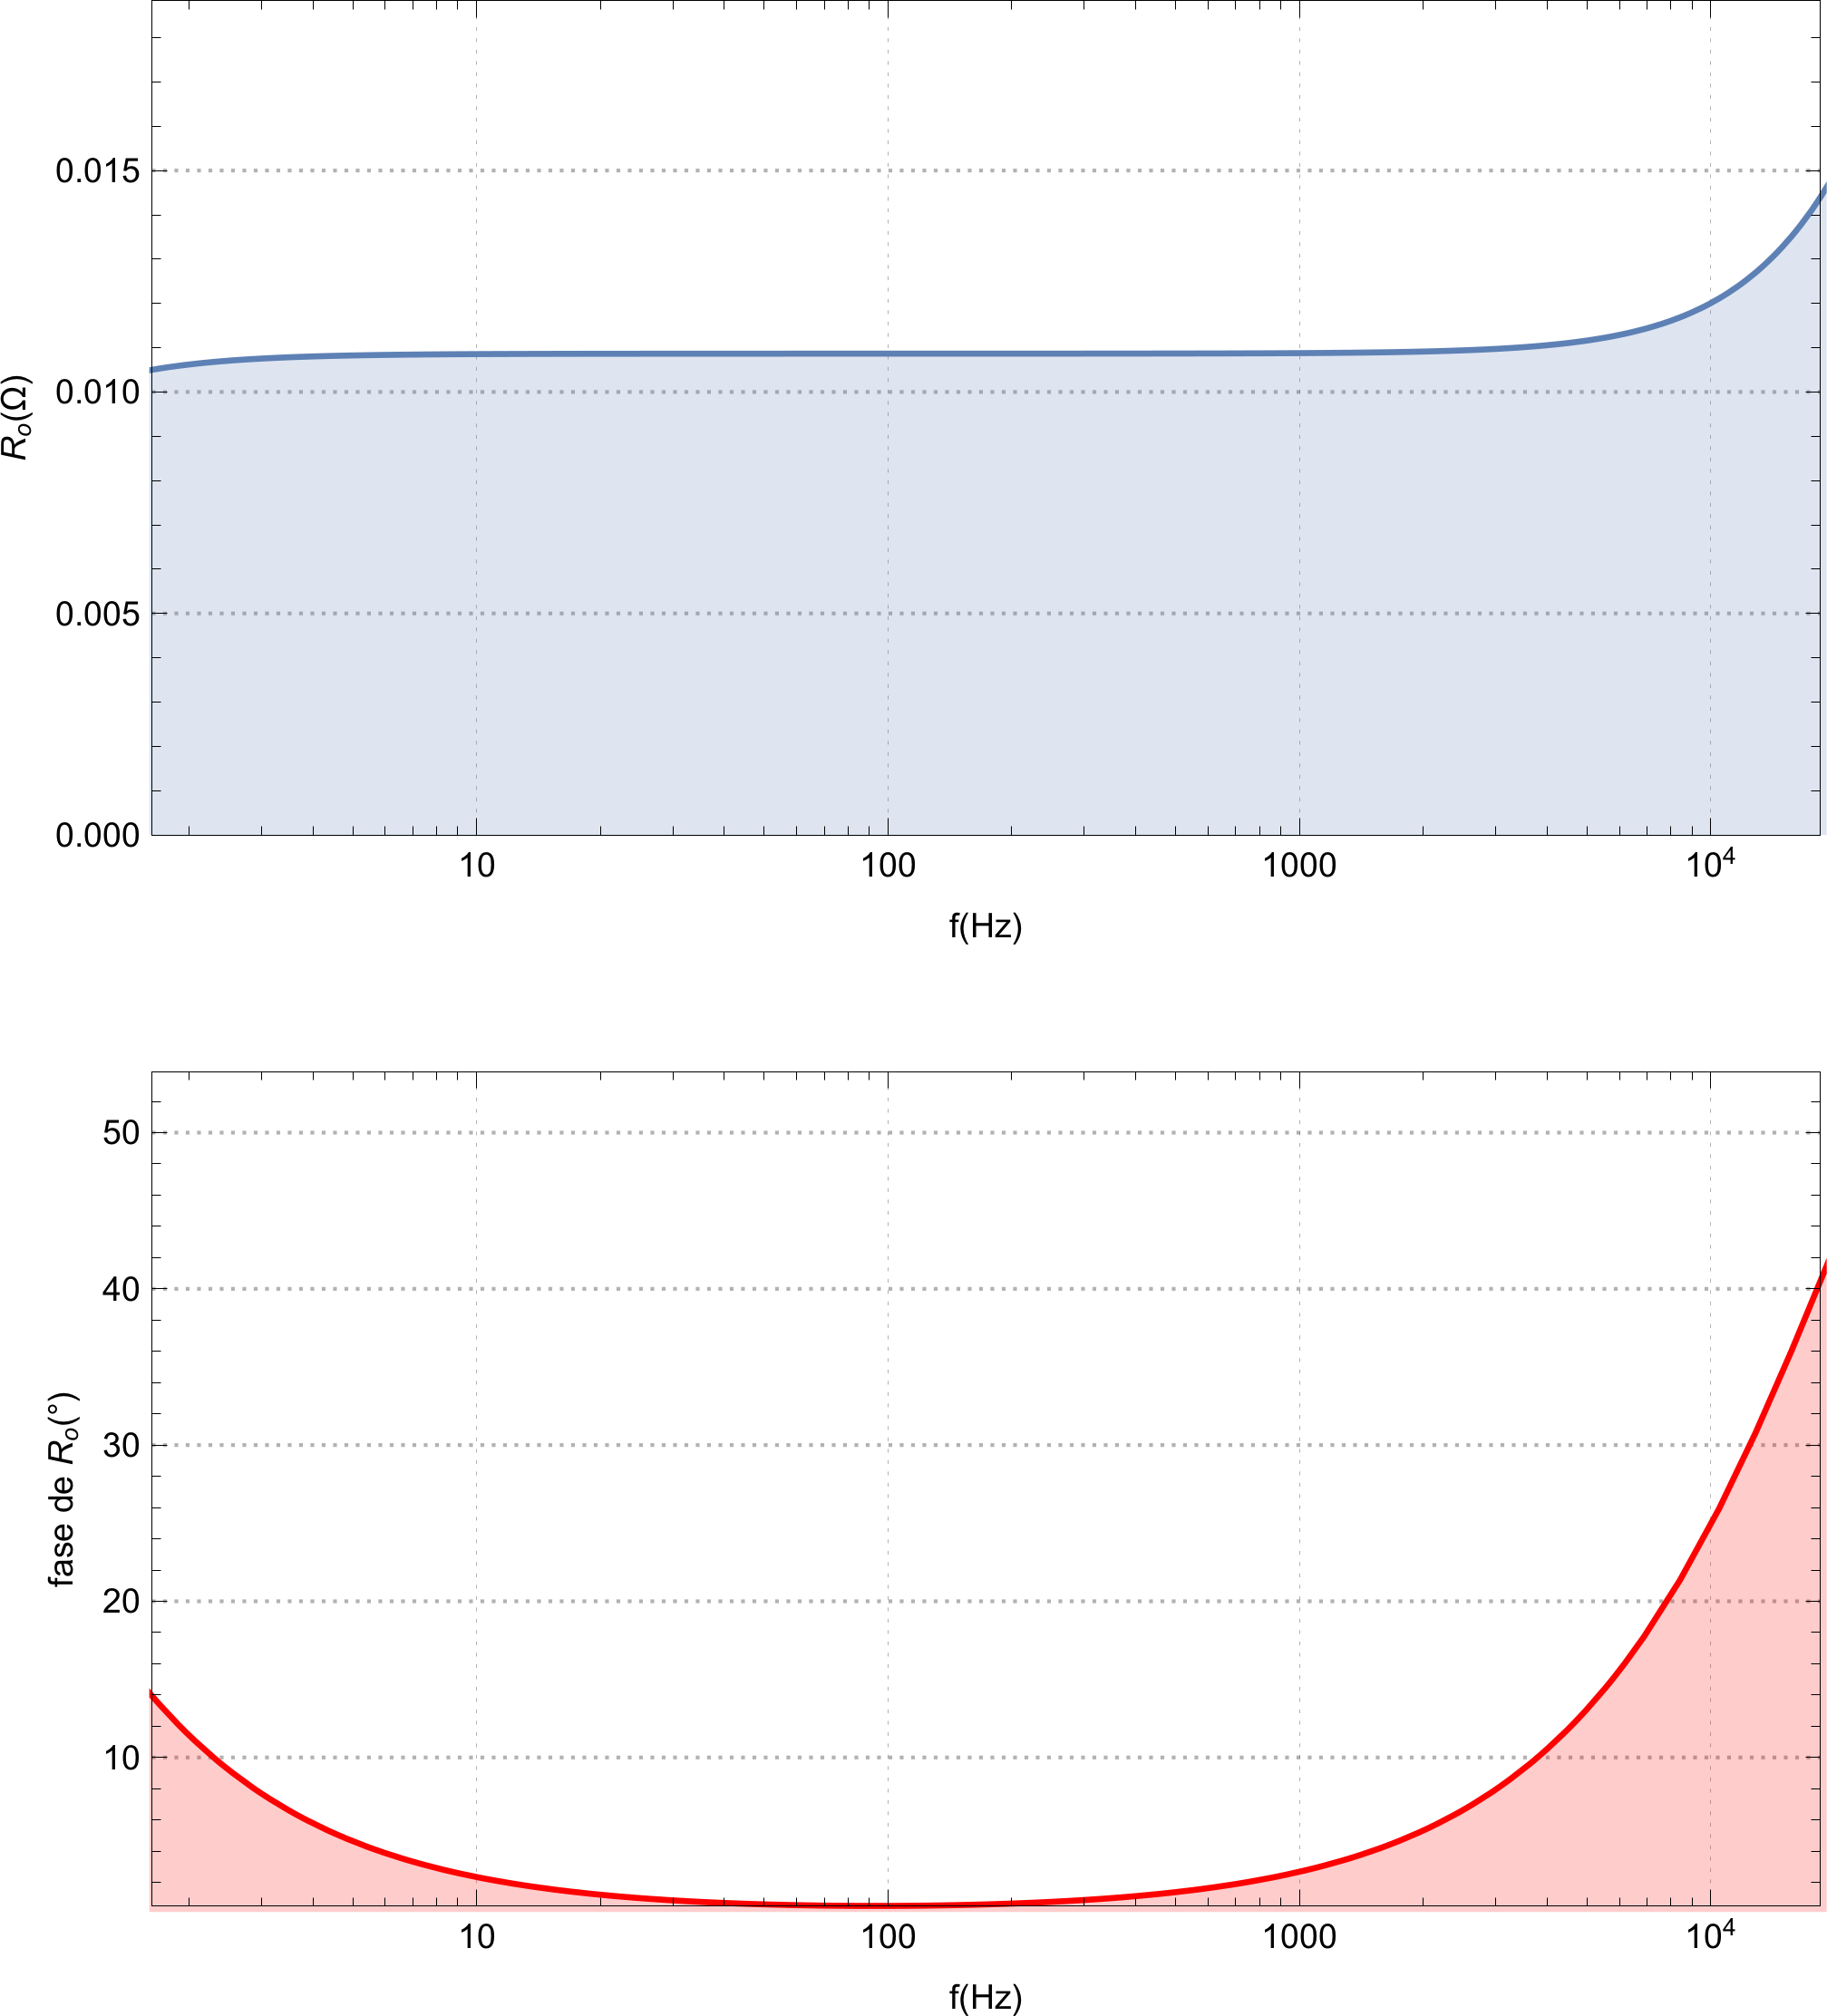
\includegraphics[width=0.8\textwidth]{img/sims/R_out-zoom.png}
	\caption{Barrido en frecuencias de la impedancia de salida simulada para frecuencias hasta $30 \si[per-mode=symbol]{\kilo\hertz}$.}
	\label{fig:R_out-zoom}
\end{figure}

El módulo de la media geométrica de la impedancia de salida para las frecuencias entre $1 \si[per-mode=symbol]{\hertz}-30 \si[per-mode=symbol]{\kilo\hertz}$ es $11 \si[per-mode=symbol]{\milli\ohm}$.

\[ R_{out}\cong 11 \si[per-mode=symbol]{\milli\ohm}\]

La realimentación global serie-paralelo logra que la resistencia de salida sea muy baja, tanto que las resistencias parásitas pueden terminar siendo un factor no despreciable. Si se desprecian, el factor de amortiguamiento es  $DP \cong 730$, cumpliendo cómodamente con lo especificado.



\subsection{Resistencia de entrada}

Se simuló en el cociente entre la tensión de entrada y la corriente entregadas por el generador, para un barrido de frecuencias. El módulo de la media geométrica de la impedancia para las frecuencias entre $1 \si[per-mode=symbol]{\hertz}-30 \si[per-mode=symbol]{\kilo\hertz}$ es $35.28 \si[per-mode=symbol]{\kilo\ohm}$.

\[ R_{in}=35.28 \si[per-mode=symbol]{\kilo\ohm} \]

En la figura~\figref{fig:R_i} se puede ver un barrido en frecuencias de la resistencia de entrada para pequeña señal.


\begin{figure}[H]
	\centering
	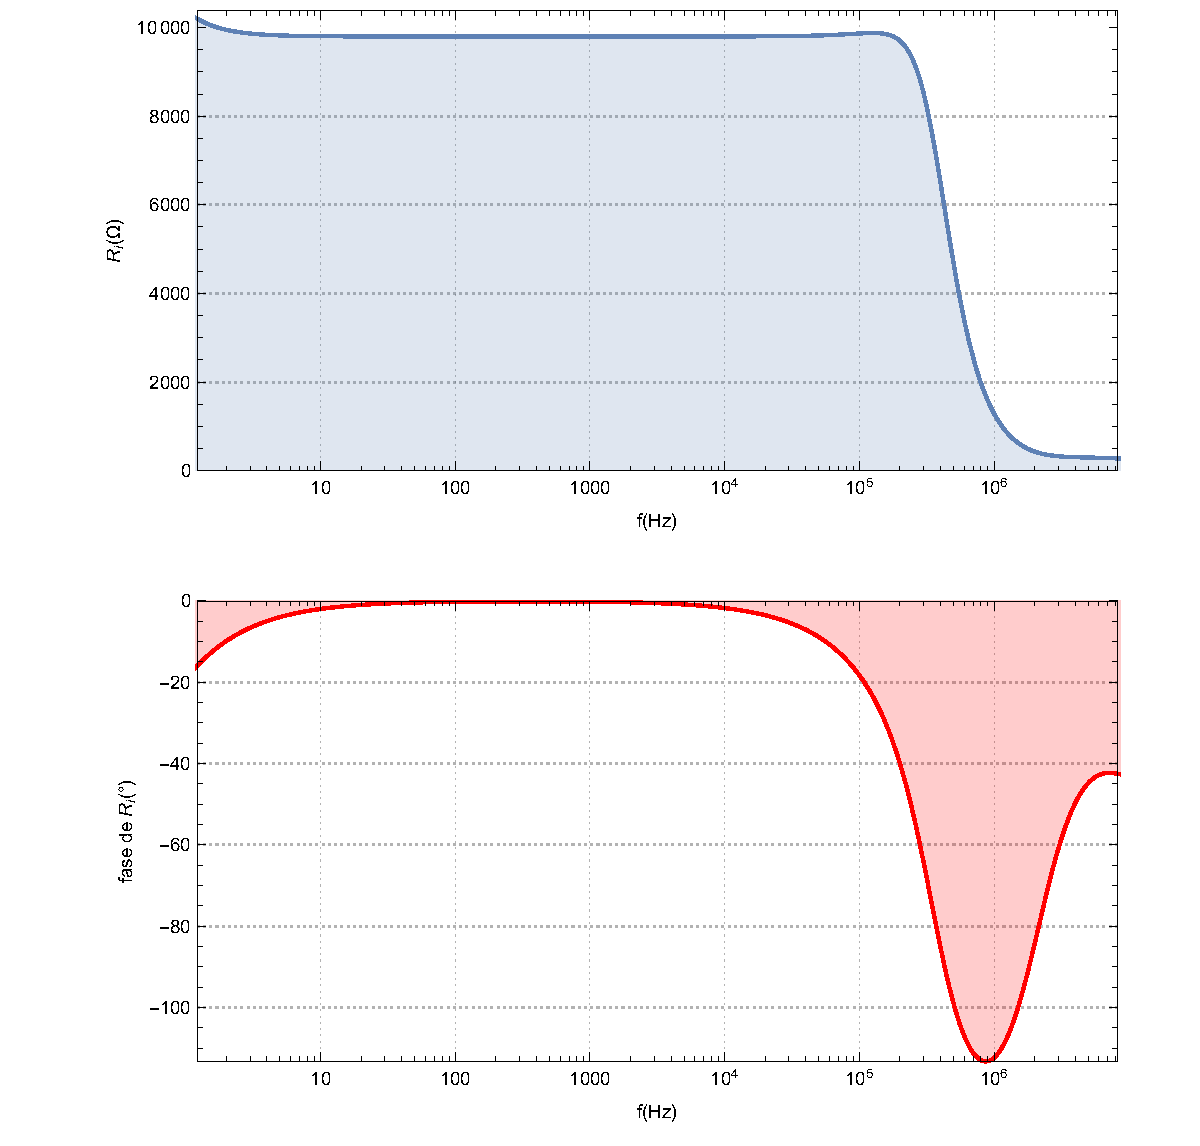
\includegraphics[width=0.8\textwidth]{img/sims/R_i.png}
	\caption{Resistencia de entrada. Cociente entre tensión y corriente de entrada simuladas para pequeña señal de distintas frecuencias.}
	\label{fig:R_i}
\end{figure}



\subsection{Ancho de banda de potencia}


En la figura~\figref{fig:power_BW} se puede observar el gráfico de módulo y fase del ancho de banda de potencia para el amplificador, el ancho de banda obtenido es de $798.45 \si[per-mode=symbol]{\kilo\hertz}$, pero como sabemos mucho antes que esta frecuencia, a $80.6 \si[per-mode=symbol]{\kilo\hertz}$, el Slew-Rate limitará la excursión del amplificador, no obstante se cumple holgadamente con la especificación establecida de  $30 \si[per-mode=symbol]{\kilo\hertz}$ de ancho de banda de potencia, aún teniendo en cuenta la limitación por Slew-Rate.


\clearpage

\begin{figure}[H]
	\centering
	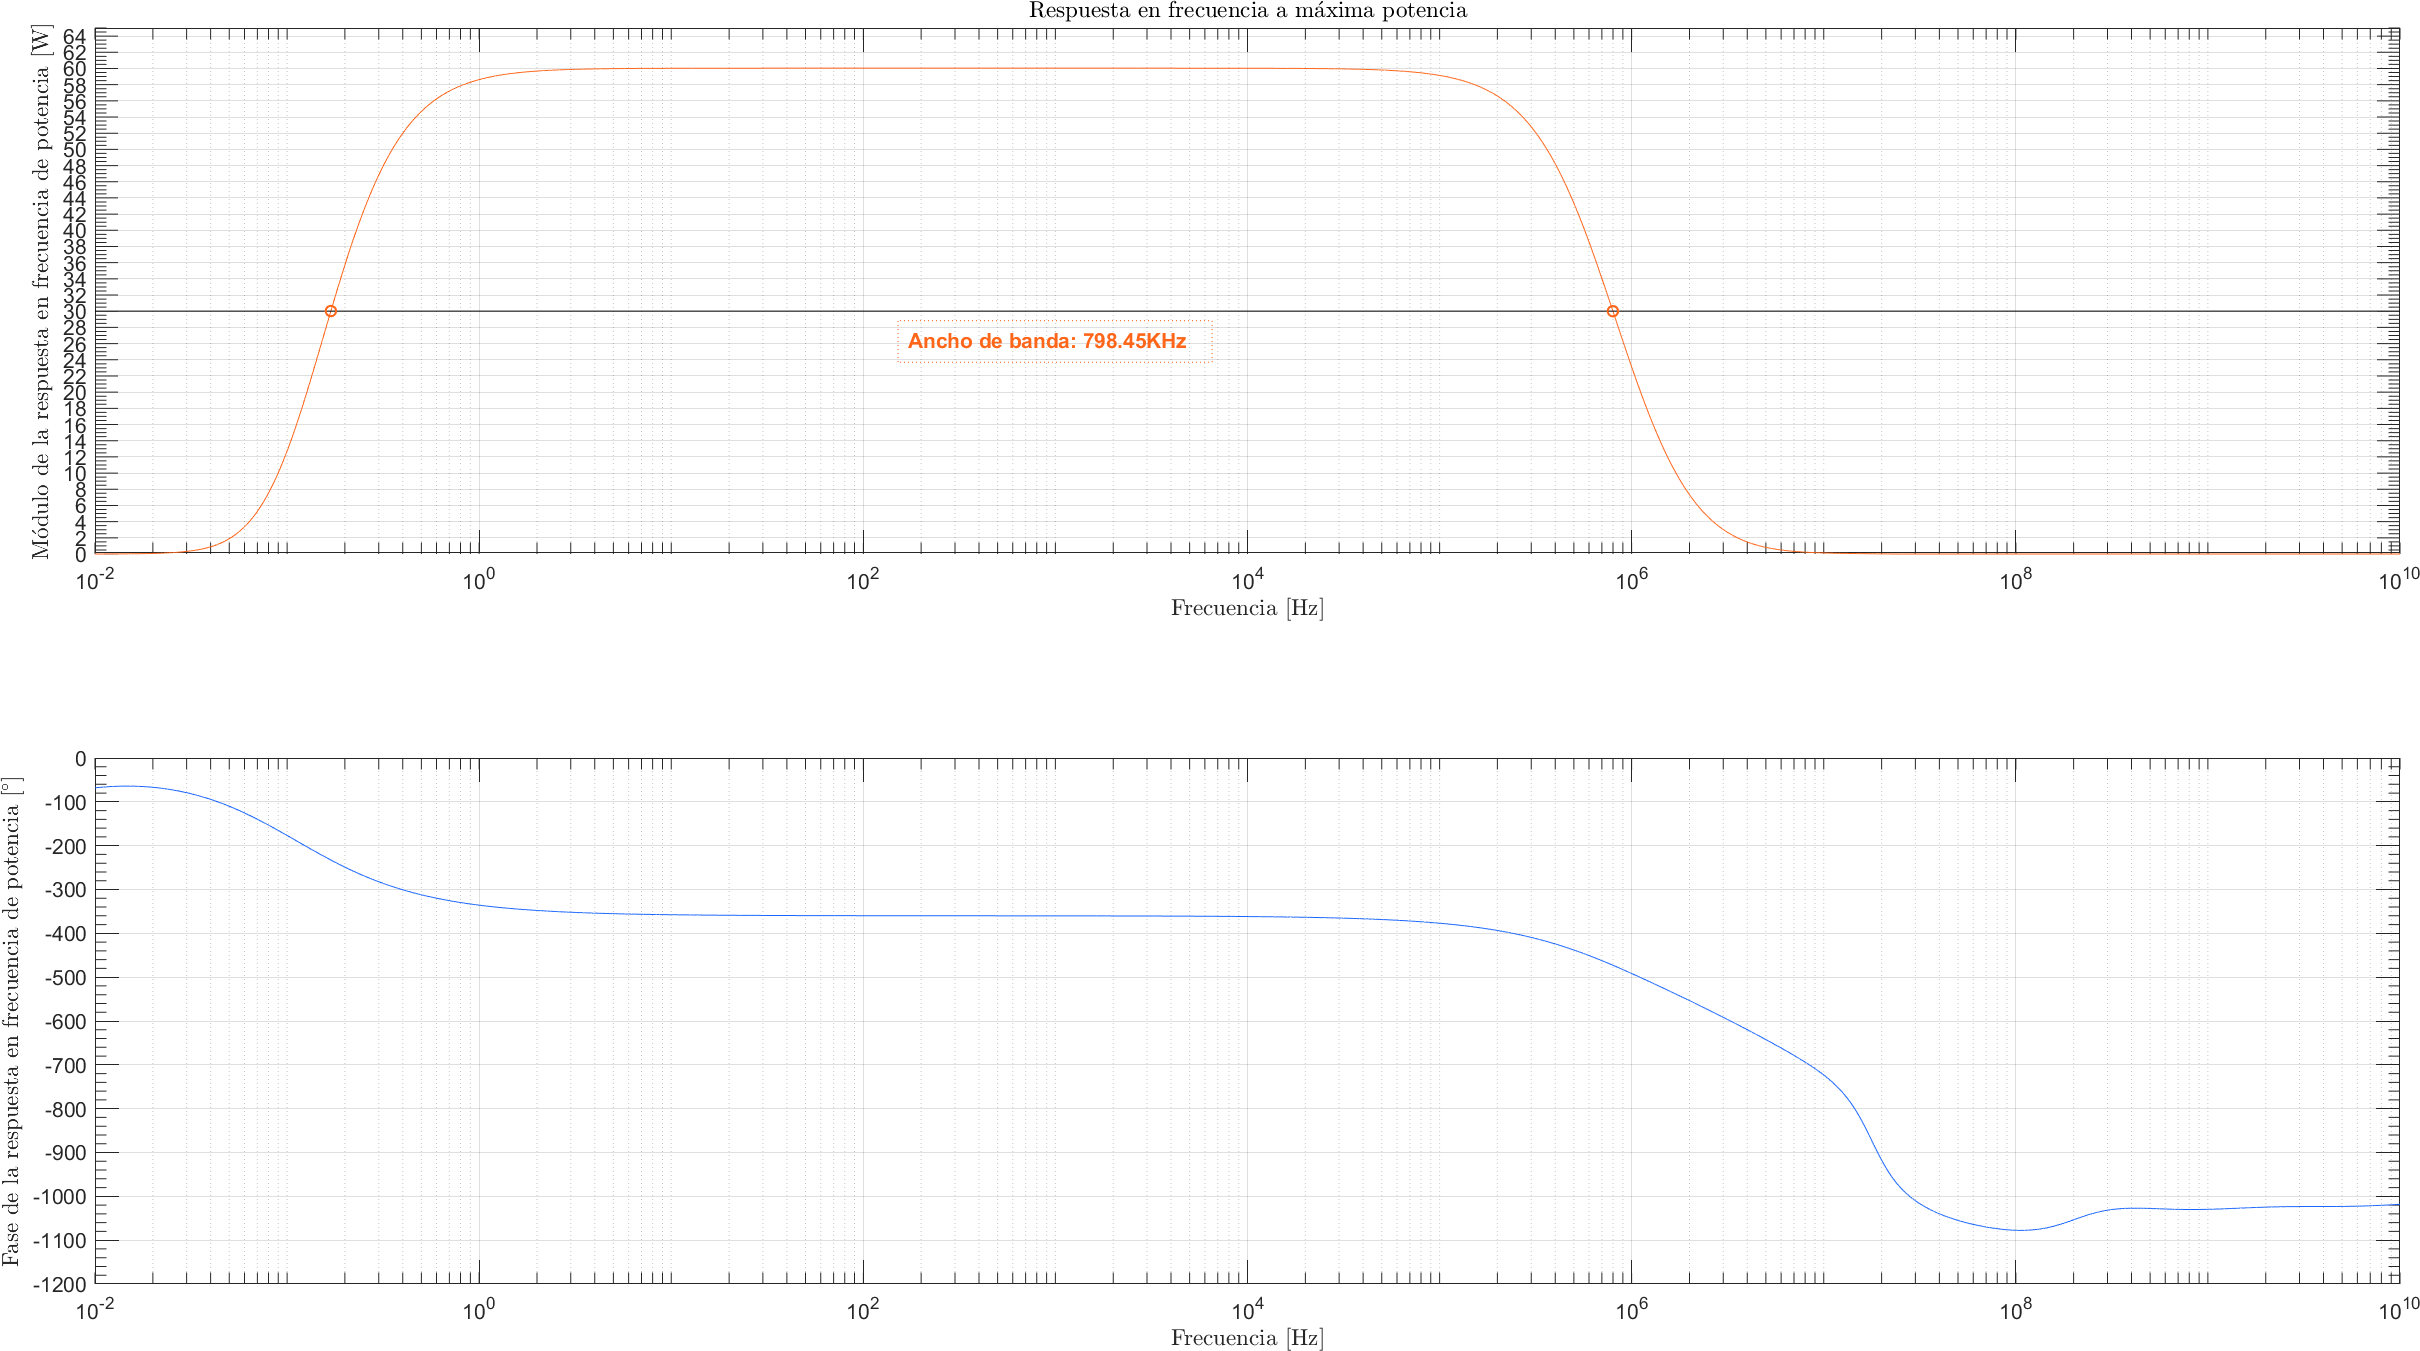
\includegraphics[width=0.7\paperheight, angle=90]{img/sims/Power_BW.png}
	\caption{Ancho de banda de potencia.}
	\label{fig:power_BW}
\end{figure}

\clearpage





\clearpage
%\\\\\\\\\\\\\\\\\\\\\\\\\\\

%\\\\\\\\\\\\\\\\\\\\\\\\\\\
\section{Alimentación}
\resetallcounters



Se colocaron capacitores ($CF_{1}$ a $CF_{8}$) en los 4 rieles de alimentación ($\pm 49 \si[per-mode=symbol]{\volt}$ y $\pm 15 \si[per-mode=symbol]{\volt}$) para filtrar ripple y ruidos en los rieles de alimentación, estos filtros se colocan cerca a la etapa de salida, y luego siguiendo las recomendaciones del libro se retorna hacia el filtro que alimenta las primeras etapas, cuidando de que los retornos sean al punto de tierra sin compartir los retornos. son pares de capacitores, uno electrolítico para filtrar principalmente el ripple de la fuente y el otro cerámico para compensar efectos inductivos y filtrar ruido de alta frecuencia introducido por el switcheo de los transistores de salida.


\subsection{Diseño de la fuente de alimentación}


\label{sec:fuente}

En nuestro proyecto vamos a utilizar una fuente no regulada con protecciones, la misma está realizada con un transformador de varias salidas, $36 \si[per-mode=symbol]{\volt} + 36 \si[per-mode=symbol]{\volt}$ y $12 \si[per-mode=symbol]{\volt} + 12 \si[per-mode=symbol]{\volt}$, otra opción son dos transformadores con punto medio independientes, ambas opciones se estudiaron y están comercialmente disponibles, en el primer caso es un diseño a medida por encargo, la decisión no hace al funcionamiento y se tomará por razones económicas y de tamaño. Los secundarios se rectifican con puentes de diodos integrados y se filtran con capacitores electrolíticos de alto valor, calculados en base a lo indicado por las simulaciones. Las protecciones consisten en limitadores de corriente, son circuitos típicos armados alrededor de un transistor bipolar con una resistencia de sensado y un \textbf{MOSFET} de potencia de paso con baja $R_{ds_{on}}$, estos circuitos se repiten para los cuatro rieles con limitaciones apropiadas en cada caso, los valores a los cuales se limitan las corrientes son suficientes para ser soportados por el tiempo necesario para quemar los fusibles en serie que tiene cada riel, de esta manera se protege al circuito de la fuente de alimentación y al amplificador, el cual tiene su propia protección para los transistores de salida, pero es muy por arriba de lo que la fuente puede entregar, ambas protecciones se complementan, evitando que ningún circuito se dañe, mas allá de los fusibles.

\vfill

\clearpage


\begin{figure}[H]
	\centering
	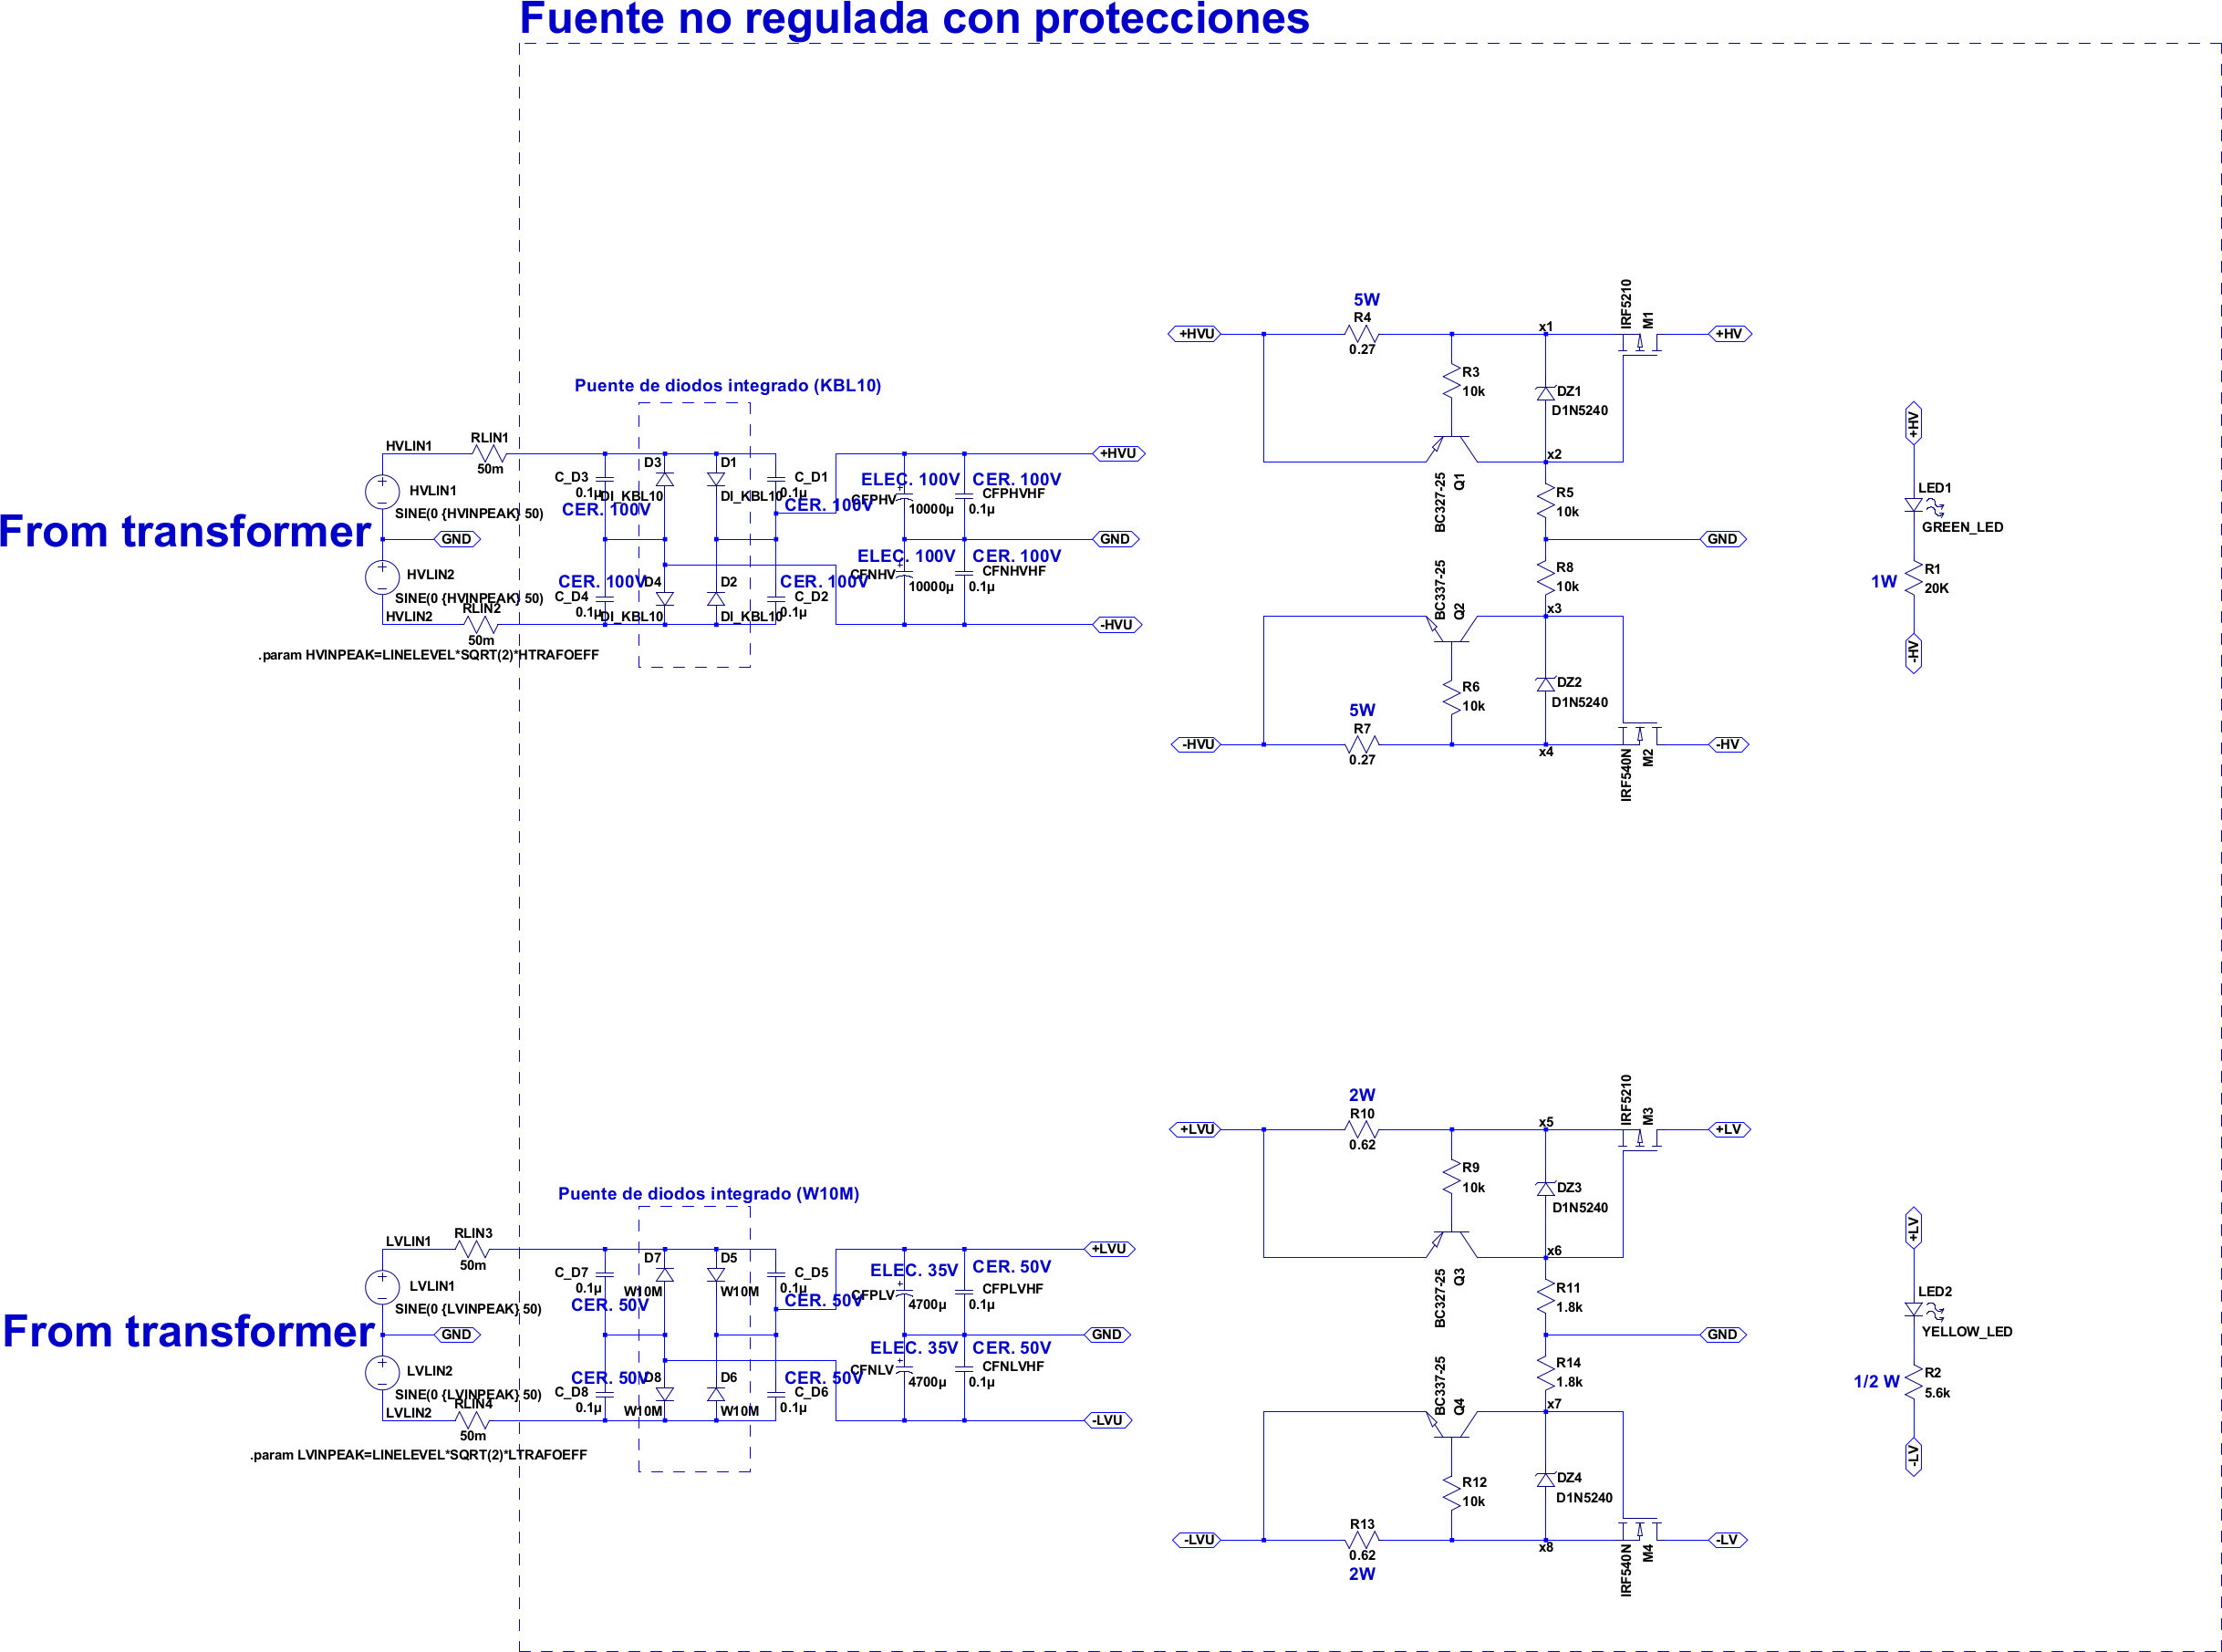
\includegraphics[width=0.7\paperheight, angle=90]{img/power_supply.png}
	\caption{Fuente de alimentación.}
	\label{fig:power_supply}
\end{figure}
\clearpage
%\\\\\\\\\\\\\\\\\\\\\\\\\\\

%\\\\\\\\\\\\\\\\\\\\\\\\\\\
\section{Diseño del pre-amplificador}
\resetallcounters

Como etapa de pre-procesamiento, elegimos un pre-amplificador relativamente sencillo que implementa, control de volumen, selección de sensibilidad para tres fuentes de audio, \textbf{consumer} (cualquier fuente de un equipo comercial, como ser un celular), \textbf{línea} (fuente de valor standard como ser la salida de una placa de sonido) y \textbf{guitarra}, además el circuito implementa un control básico de tonos, con control de \textbf{Bass} y \textbf{Trebel}, con lo cual se tiene una llave selectora de tres puntos, un potenciómetro logarítmico para el volumen y dos potenciómetros lineales para el control de tonos. Para la implementación se necesitan tres amplificadores operacionales, para esta función seleccionamos el operacional \textbf{NE5532} de \textbf{Texas}, por su diseño específico para audio y su bajo ruido. El circuito es simple, la primer etapa es un atenuador conectado a la entrada de un amplificador no inversor, acoplado capacitivamente, la segunda etapa es un operacional con dos redes de realimentación para atenuar o graves alrededor de $100 \si[per-mode=symbol]{\hertz}$ o agudos alrededor de $10 \si[per-mode=symbol]{\kilo\hertz}$, el circuito original amplificaba, pero para adecuarlo a la sensibilidad de nuestro amplificador lo modificamos para que siempre la salida esté por debajo de $\si[per-mode=symbol]{1.1 \volt}$, para esto el circuito cuenta con una serie de presets en la etapa de salida que permiten ajustar el selector de sensibilidades y la ganancia global para adaptarse perfectamente a nuestro amplificador.


\vfill

\clearpage


\begin{figure}[H]
	\centering
	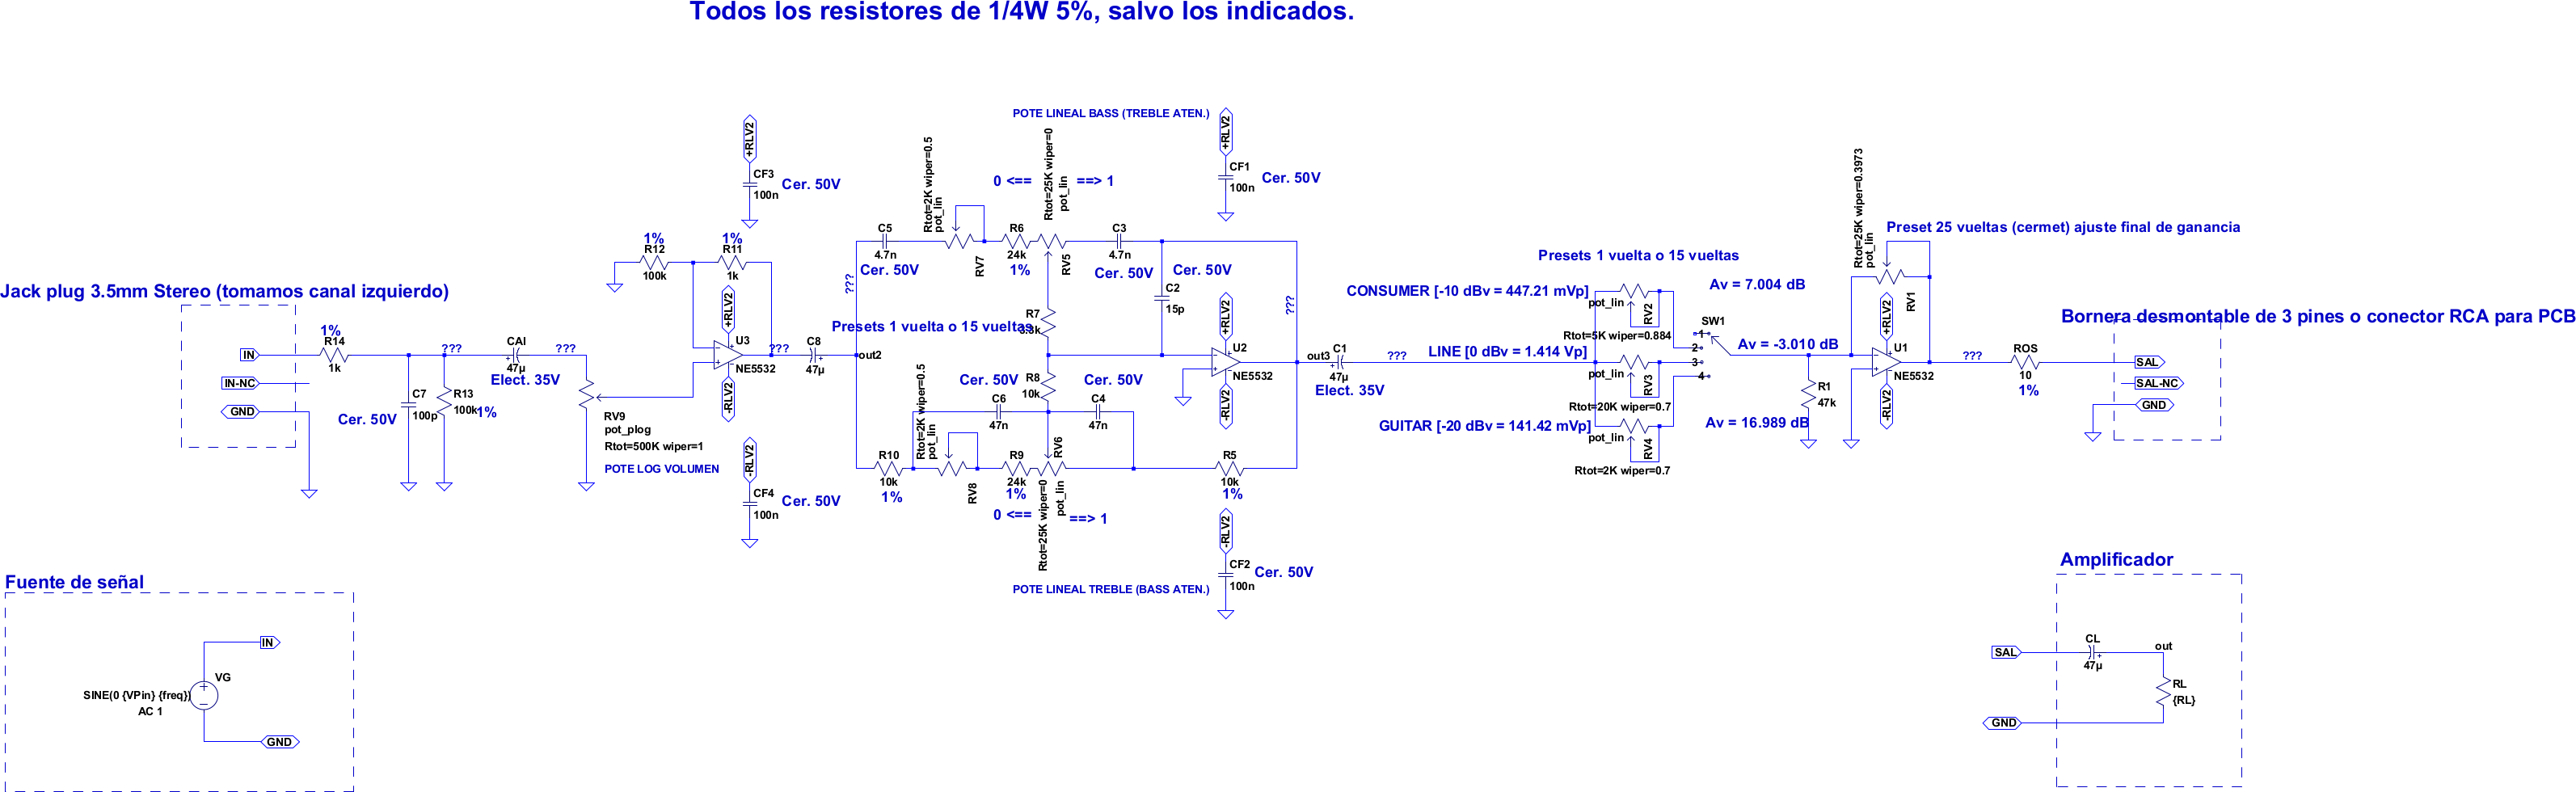
\includegraphics[width=0.7\paperheight, angle=90]{img/preamp.png}
	\caption{pre-amplificador con control de tonos y volumen.}
	\label{fig:power_supply}
\end{figure}
\clearpage
%\\\\\\\\\\\\\\\\\\\\\\\\\\\


%\\\\\\\\\\\\\\\\\\\\\\\\\\\
\section{Diseño de PCB}
\resetallcounters

\subsection{Lista de materiales}

\begin{table}[h!]
\centering

\label{BOM}


\resizebox{0.99 \textwidth}{!}{

\begin{tabular}{|l|l|l|l|l|l|l|l|l|}
\hline
	Descripción & Nombre & Referencia & Potencia & Cantidad & Tipo & Tensión & Tensión de zener & Tolerancia \\ \hline
	TERMI-BLOK HEADER,ASSY90 2P - serie 282822 - 5.00mm & B1 & C-282822-2-C &  & 1 &  &  &  &  \\ \hline
	TERMI-BLOK HEADER,ASSY90 2P - serie 282822 - 5.00mm & B2 & C-282822-2-C &  & 1 &  &  &  &  \\ \hline
	TERMI-BLOK HEADER,ASSY90 2P - serie 282822 - 5.00mm & B3 & C-282822-2-C &  & 1 &  &  &  &  \\ \hline
	TERMI-BLOK HEADER,ASSY90 2P - serie 282822 - 5.00mm & B4 & C-282822-2-C &  & 1 &  &  &  &  \\ \hline
	TE Barrier Terminal Block, 2P & BO & 8PCV-02-006 &  & 1 &  & 600V &  &  \\ \hline
	Aluminum Electrolytic Capacitor 1000μF 16V 20\% 105º & CAF & Al. Elect. 1000u 16V 20\% 105º &  & 1 &  & 16V &  & 20\% \\ \hline
	Aluminum Electrolytic Capacitor 47μF 35V 20\% 105º & CAI & Al. Elect. 47u 35V 20\% 105º &  & 1 &  & 35V &  & 20\% \\ \hline
	Ceramic Capacitor 10nF 50V 10\% & CC1 & Cer. 10n 50V 10\% &  & 1 &  & 50V &  & 10\% \\ \hline
	Ceramic Capacitor 6.8nF 50V 10\% & CC2 & Cer. 6.8n 50V 10\% &  & 1 &  & 50V &  & 10\% \\ \hline
	Ceramic Capacitor 68pF 50V 10\% & CC3, CC4 & Cer. 68p 50V 10\% &  & 2 &  & 50V &  & 10\% \\ \hline
	Ceramic Capacitor 100pF 50V 10\% & CC5, CC6 & Cer. 100p 50V 10\% &  & 2 &  & 50V &  & 10\% \\ \hline
	Ceramic Capacitor 1.2pF 50V 10\% & CC7 & Cer. 1.2p 50V 10\% &  & 1 &  & 50V &  & 10\% \\ \hline
	Aluminum Electrolytic Capacitor 220μF 16V 20\% 85º & CCF32, CF31 & Al. Elect. 220u 16V 20\% 85º &  & 2 &  & 16V &  & 20\% \\ \hline
	Aluminum Electrolytic Capacitor 470μF 100V 20\% 105º & CF1, CF2, CF3, CF4, CF9, CF10 & Al. Elect. 470u 100V 20\% 105º &  & 6 &  & 100V &  & 20\% \\ \hline
	Polyester Capacitor 100nF 100V 10\% & CF5, CF6, CF7, CF8, CF11, CF12 & Poly. 100n 100V 10\% &  & 6 &  & 100V &  & 10\% \\ \hline
	Ceramic Capacitor 100nF 50V 10\% & CF33, CF34, CF37, CF38 & Cer. 100n 50V 10\% &  & 4 &  & 50V &  & 10\% \\ \hline
	Aluminum Electrolytic Capacitor 220μF 35V 20\% 105º & CF35, CF36 & Al. Elect. 220u 35V 20\% 105º &  & 2 &  & 35V &  & 20\% \\ \hline
	Tantalum Electrolytic Capacitor 1μF 25V 10\% & CF39, CF40 & Tant. Elect. 1u 25V 10\% &  & 2 &  & 25V &  & 10\% \\ \hline
	45 V, 16 A SWITCHMODE(TM) Schottky Power Rectifier, 2-Pin TO-220, Pb-Free, Tube & D1, D2 & MBR1645 &  & 2 &  &  &  &  \\ \hline
	FAST SWITCHING DIODE & D3, D4 & 1N4148 & 400mW & 2 &  &  &  &  \\ \hline
	FAST SWITCHING DIODE & D5, D6, D31, D32, D33, D34 & 1N4148 & 400mW & 6 &  &  &  &  \\ \hline
	SURFACE MOUNT FAST SWITCHING DIODE & D35, D36, D37, D38 & 1N4148W & 400mW & 4 &  &  &  &  \\ \hline
	Zener Diode, 2.7V, 500mW & DZ1, DZ2 & 1N4371A & 500mW & 2 &  &  & 2.7V &  \\ \hline
	Zener Diode, 22V, 500mW & DZ3, DZ4 & 1N969B & 500mW & 2 &  &  & 22V &  \\ \hline
	5V fixed regulator - 100mA & IC1 & LM78L05 &  & 1 &  &  &  &  \\ \hline
	-5V fixed regulator - 100mA & IC2 & LM79L05 &  & 1 &  &  &  &  \\ \hline
	Conn Phono Jack F 3 POS Solder RA Thru-Hole 3 Terminal 1 Port & JI & PJRAN1X1U01X &  & 1 &  &  &  &  \\ \hline
	Jumper Wire & JU1, JU2, JU3, JU4 & Jumper\_3pin &  & 4 &  &  &  &  \\ \hline
	Jumper Wire & JU5 & Jumper &  & 1 &  &  &  &  \\ \hline
	Typical LED (GREEN) & LED1 & LED (GREEN) &  & 1 &  &  &  &  \\ \hline
	Typical LED (YELLOW) & LED2 & LED (YELLOW) &  & 1 &  &  &  &  \\ \hline
	Transistor GP BJT NPN 230V 15A 3-Pin\_3+Tab\_ TO-264 Tube & Q1, Q3, Q5 & 2SC5200 & 150W & 3 &  &  &  &  \\ \hline
	Transistor GP BJT PNP 230V 15A 3-Pin\_3+Tab\_ TO-264 Tube & Q2, Q4, Q6 & 2SA1943 & 150W & 3 &  &  &  &  \\ \hline
	Plastic Medium-Power NPN Silicon Transistor, 300 VOLTS, 0.5 AMPERE, 20 WATTS & Q7, Q9, Q15, Q16, Q19 & MJE340G & 20W & 5 &  &  &  &  \\ \hline
	Plastic Medium-Power PNP Silicon Transistor, 300 VOLTS, 0.5 AMPERE, 20 WATTS & Q8, Q10, Q20 & MJE350G & 20W & 3 &  &  &  &  \\ \hline
	High Voltage NPN Bipolar Transistor & Q11, Q18 & MPSA42 & 20W & 2 &  &  &  &  \\ \hline
	High Voltage PNP Bipolar Transistor & Q12, Q17 & MPSA92 & 20W & 2 &  &  &  &  \\ \hline
	High Voltage NPN Bipolar Transistor & Q31, Q35, Q37 & MMBTA42 & 20W & 3 &  &  &  &  \\ \hline
	High Voltage PNP Bipolar Transistor & Q32, Q36, Q38 & MMBTA92 & 20W & 3 &  &  &  &  \\ \hline
	Quad NPN and PNP General-Purpose Amplifier & QI & MMPQ6700 & 180mW & 1 &  &  &  &  \\ \hline
	Resistor 0.1$\Omega$ 2W 5\% & R1, R2, R5, R6 & Resistor 0.1 2W 5\% & 2W & 4 & (TH) Carbon film &  &  & 5\% \\ \hline
	Cemented resistor 0.15$\Omega$ 5\% 5W & R3, R4 & Cemented resistor 0.15 5W 5\% & 5W & 2 & (TH) Wired cemented &  &  & 5\% \\ \hline
	Resistor 68$\Omega$ 1/4W 1\% & R7, R8 & Resistor 68 1/4W 1\% & 1/4W & 2 & (TH) Metal film &  &  & 1\% \\ \hline
	Resistor 100$\Omega$ 1/4W 1\% & R9, R10, R11, R12, R17, R18 & Resistor 100 1/4W 1\% & 1/4W & 6 & (TH) Metal film &  &  & 1\% \\ \hline
	Resistor 22K$\Omega$ 1/4W 1\% & R13, R14 & Resistor 22K 1/4W 1\% & 1/4W & 2 & (TH) Metal film &  &  & 1\% \\ \hline
	Resistor 30$\Omega$ 1/4W 1\% & R15, R16 & Resistor 30 1/4W 1\% & 1/4W & 2 & (TH) Metal film &  &  & 1\% \\ \hline
	Resistor 360$\Omega$ 1/4W 1\% & R19, R20 & Resistor 360 1/4W 1\% & 1/4W & 2 & (TH) Metal film &  &  & 1\% \\ \hline
	Resistor 510$\Omega$ 1/4W 1\% & R21, R22 & Resistor 510 1/4W 1\% & 1/4W & 2 & (TH) Metal film &  &  & 1\% \\ \hline
	Resistor 16K$\Omega$ 1/4W 1\% & R31, R32 & Resistor 16K 1/4W 1\% & 1/4W & 2 & (TH) Metal film &  &  & 1\% \\ \hline
	RES 150R SM0805 YAGEO RC\_L & R33, R34 & RC0805FR-07150RL &  & 2 &  &  &  &  \\ \hline
	Resistor 15K$\Omega$ 1/4W 1\% & R35, R36 & Resistor 15K 1/4W 1\% & 1/4W & 2 & (TH) Metal film &  &  & 1\% \\ \hline
	RES 1K2 SM0603 YAGEO RC\_L & R37, R38 & RC0603FR-071K2L &  & 2 &  &  &  &  \\ \hline
	Resistor 15$\Omega$ 1/4W 1\% & RF1, RF2 & Resistor 15 1/4W 1\% & 1/4W & 2 & (TH) Metal film &  &  & 1\% \\ \hline
	Resistor 36K$\Omega$ 1/4W 1\% & RFB1, RIOF & Resistor 36K 1/4W 1\% & 1/4W & 2 & (TH) Metal film &  &  & 1\% \\ \hline
	Resistor 1.3k$\Omega$ 1/4W 1\% & RFB2 & Resistor 1.3k 1/4W 1\% & 1/4W & 1 & (TH) Metal film &  &  & 1\% \\ \hline
	Resistor 20K$\Omega$ 1W 5\% & RL1 & Resistor 20K 1W 5\% & 1W & 1 & (TH) Carbon film &  &  & 5\% \\ \hline
	Resistor 5.6K$\Omega$ 1/2W 5\% & RL2 & Resistor 5.6K 1/2W 5\% & 1/2W & 1 & (TH) Metal film &  &  & 5\% \\ \hline
	Resistor 1.2k$\Omega$ 1/4W 1\% & RMVM & Resistor 1.2k 1/4W 1\% & 1/4W & 1 & (TH) Metal film &  &  & 1\% \\ \hline
	Trimmer Vertical 100 500mW 25-turn & RV1, RV2 & RES\_TRIMMER\_100\_25T\_VERTICAL &  & 2 &  &  &  & ±10\% \\ \hline
	Trimmer Vertical 2K 500mW 25-turn & RVC1, RVC2 & RES\_TRIMMER\_2K\_25T\_VERTICAL &  & 2 &  &  &  & ±10\% \\ \hline
	Trimmer Vertical 1K 500mW 25-turn & RVMV & RES\_TRIMMER\_1K\_25T\_VERTICAL &  & 1 &  &  &  & ±10\% \\ \hline
	Test Point PCB mount Multi-purpose Black & \makecell{ TP-HV, TP-LV, TP-RLV, TP+HV, \\ TP+LV, TP+RLV, TP1, TP2, \\ TP3, TP5, TP6, TP7, \\ TP8, TP9, TP10, TP11, \\ TP12, TPGND, TPIN, TPOUT } & TESTPOINT\_THT &  & 21 &  &  &  &  \\ \hline
	Jumper Wire & TPMIDMV & Pin &  & 1 &  &  &  &  \\ \hline
\end{tabular}


}
\caption{Lista de materiales}
\end{table}


\subsection{Consideraciones al diseñar los PCB}


\subsubsection{Fuentes de Ruido Intrínsecas}

En esta subsección se analizan los distintos tipos de ruidos presentes en el amplificador.

\paragraph{Ruido Térmico o Ruido Johnson}

Es producido por los movimientos aleatorios de los electrones en componentes que disipan energía (resistores, transistores).

\paragraph{Ruido Shot}

Es el ruido asociado a la circulación de corriente a través de una barrera de potencial y es proporcional a la corriente en continua que circula. Por lo tanto, para reducir este tipo de ruido es necesario mantener la corriente DC lo más pequeña posible. Por esto se intento bajar las corrientes de polarizacion del par diferencial.

\paragraph{Ruido Popcorn}

Asociado a deficiencias en el proceso de fabricación de semiconductores. En el diseño no se tiene control sobre este tipo de ruido.



\subsubsection{Capacitancias parásitas}


Por pistas y planos en PCB:
\newline
\newline
A la hora de diseñar el PCB se tuvieron en cuenta muchas de las técnicas para reducir estos efectos. Sin embargo estos efectos no se pueden evitar al 100\%. Esos efectos deberían ser mínimos; los mismos van a ser medidos y compensados en el momento de tener el PCB fabricado.

\clearpage


\subsection{PCB del amplificador}

En las siguientes páginas se incluyen las capas del PCB del amplificador diseñado en Altium, ver archivo adjunto, \textbf{\quotemarks{PCBS-3D.pdf}} para una vista 3D interactiva del PCB.

\clearpage

\begin{figure}[H]
    \centering
    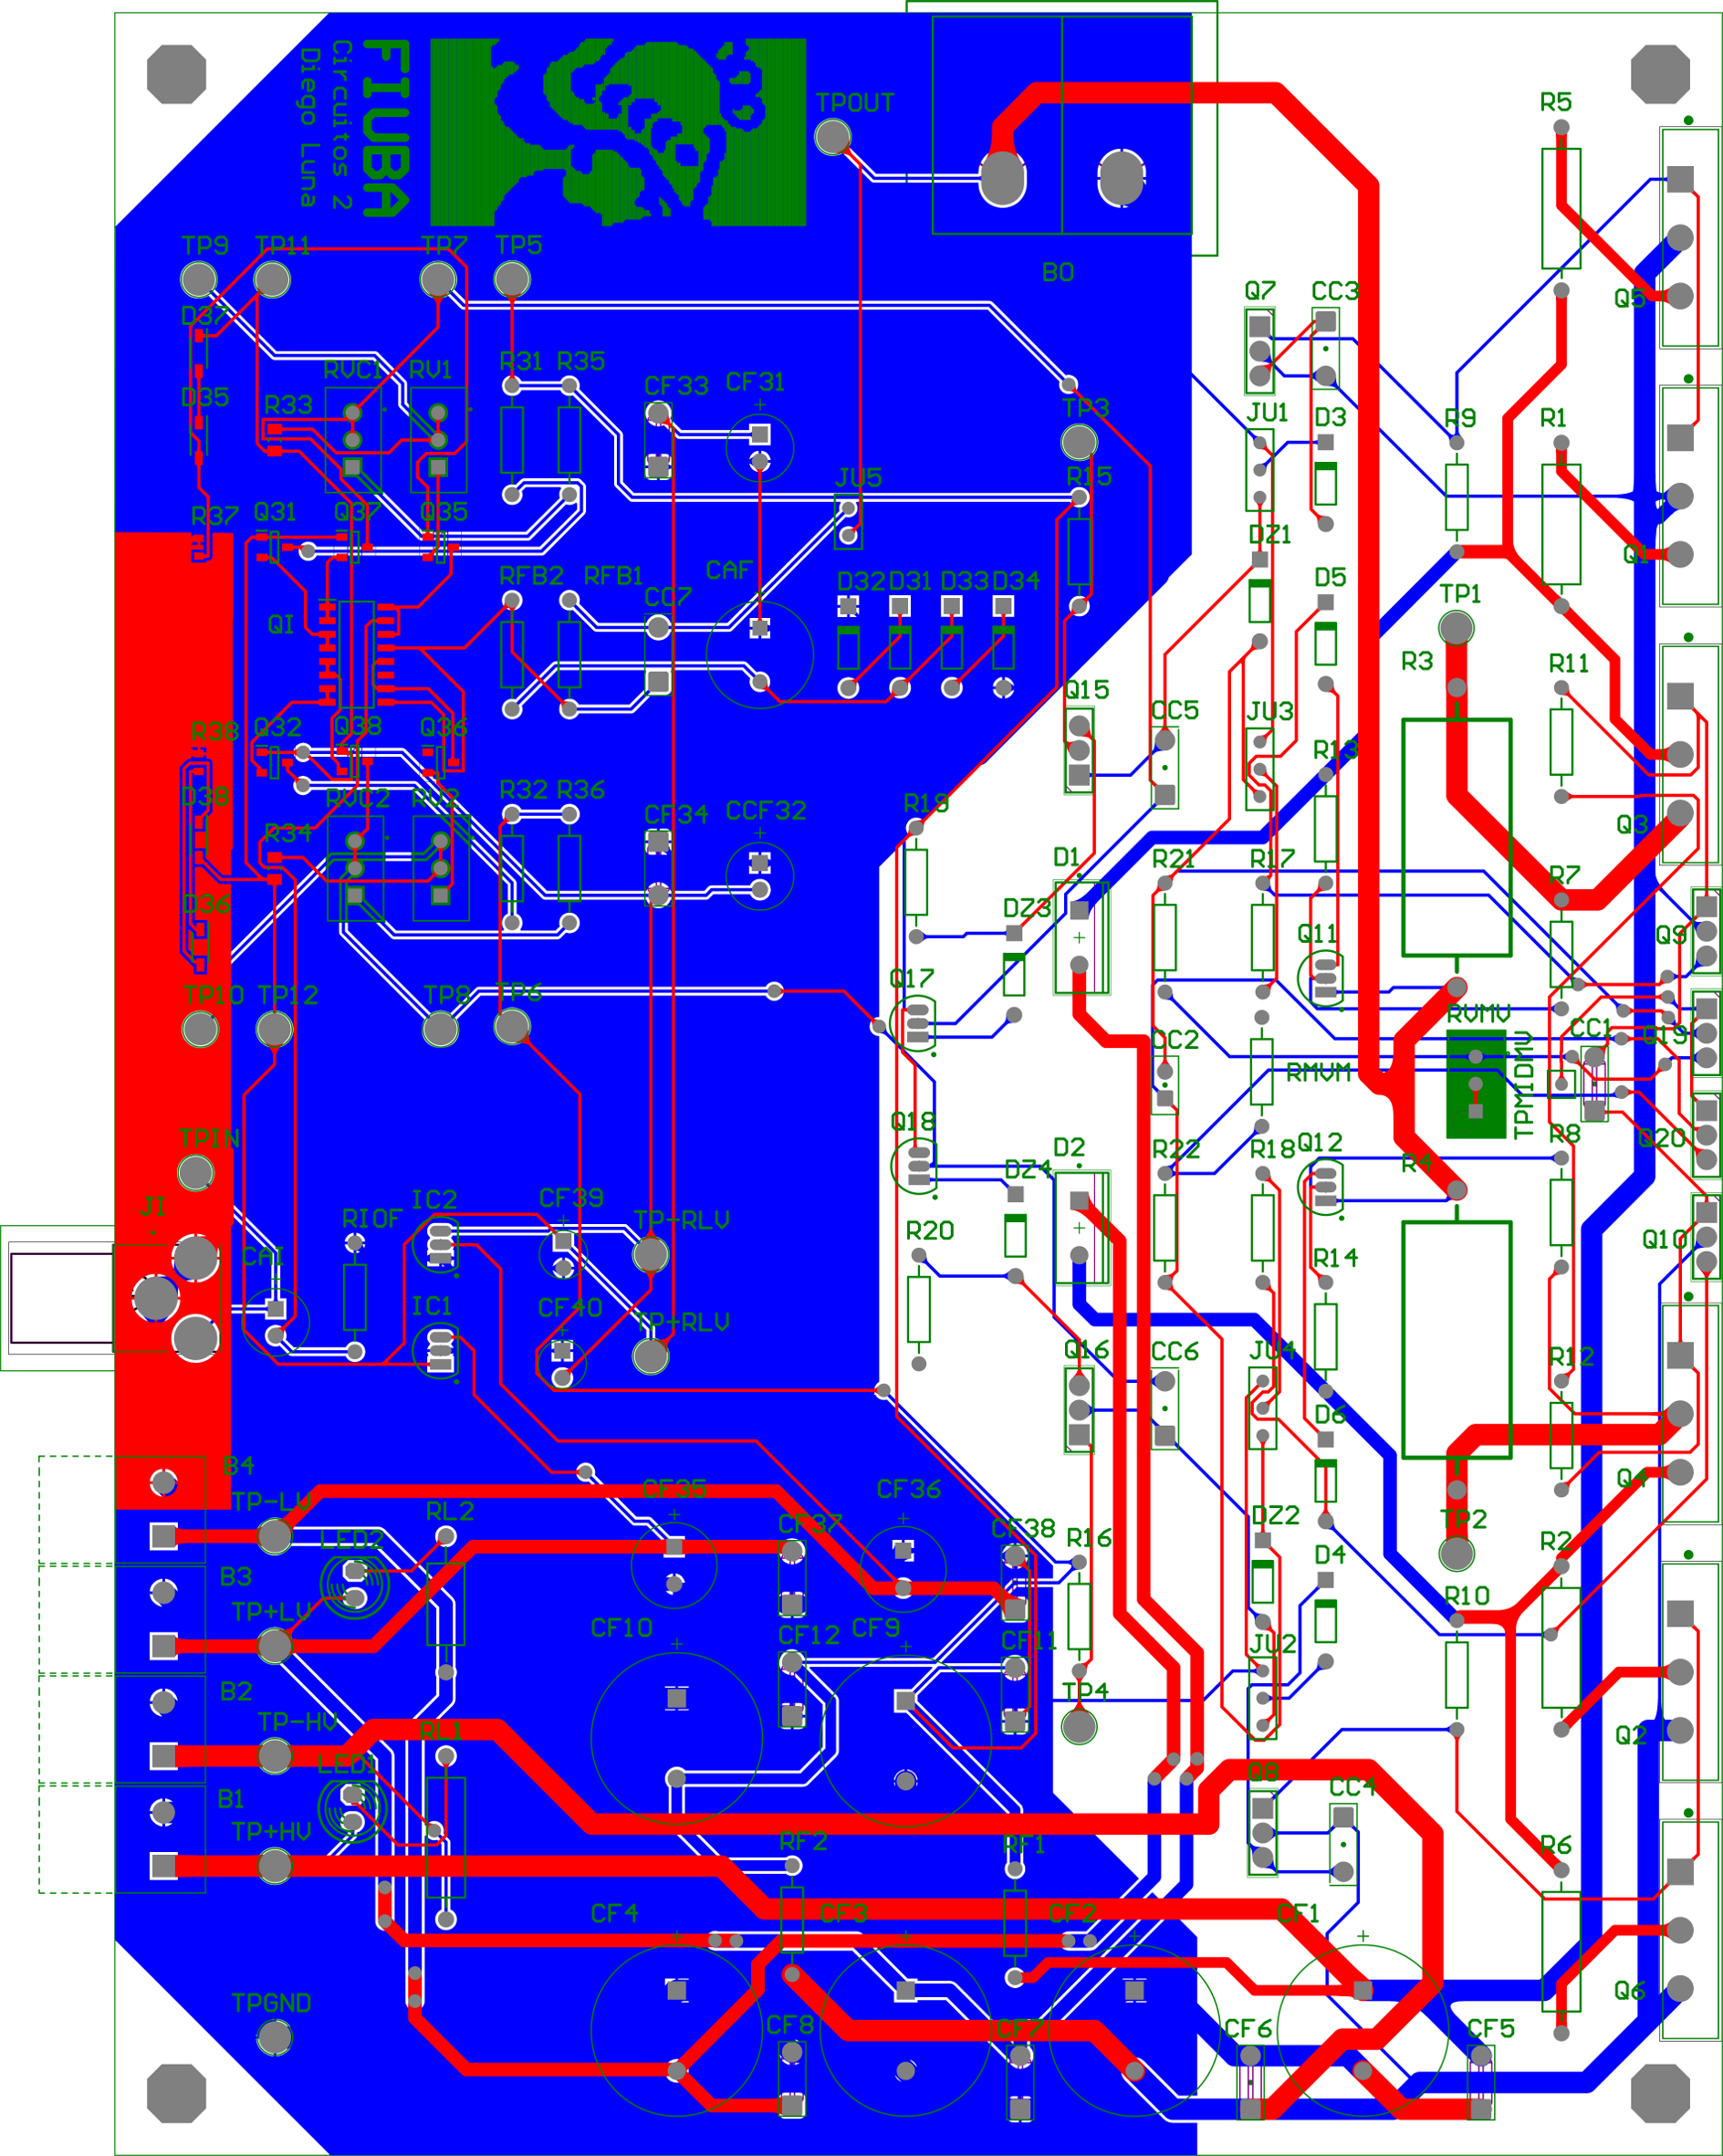
\includegraphics[height=200mm, angle=0]{img/PCB/layers/amplifier/all-2D.png}
    \caption{\footnotesize{Todas las capas}}
    \label{fig:pcb_amp_all}
\end{figure}

\clearpage

\begin{figure}[H]
    \centering
    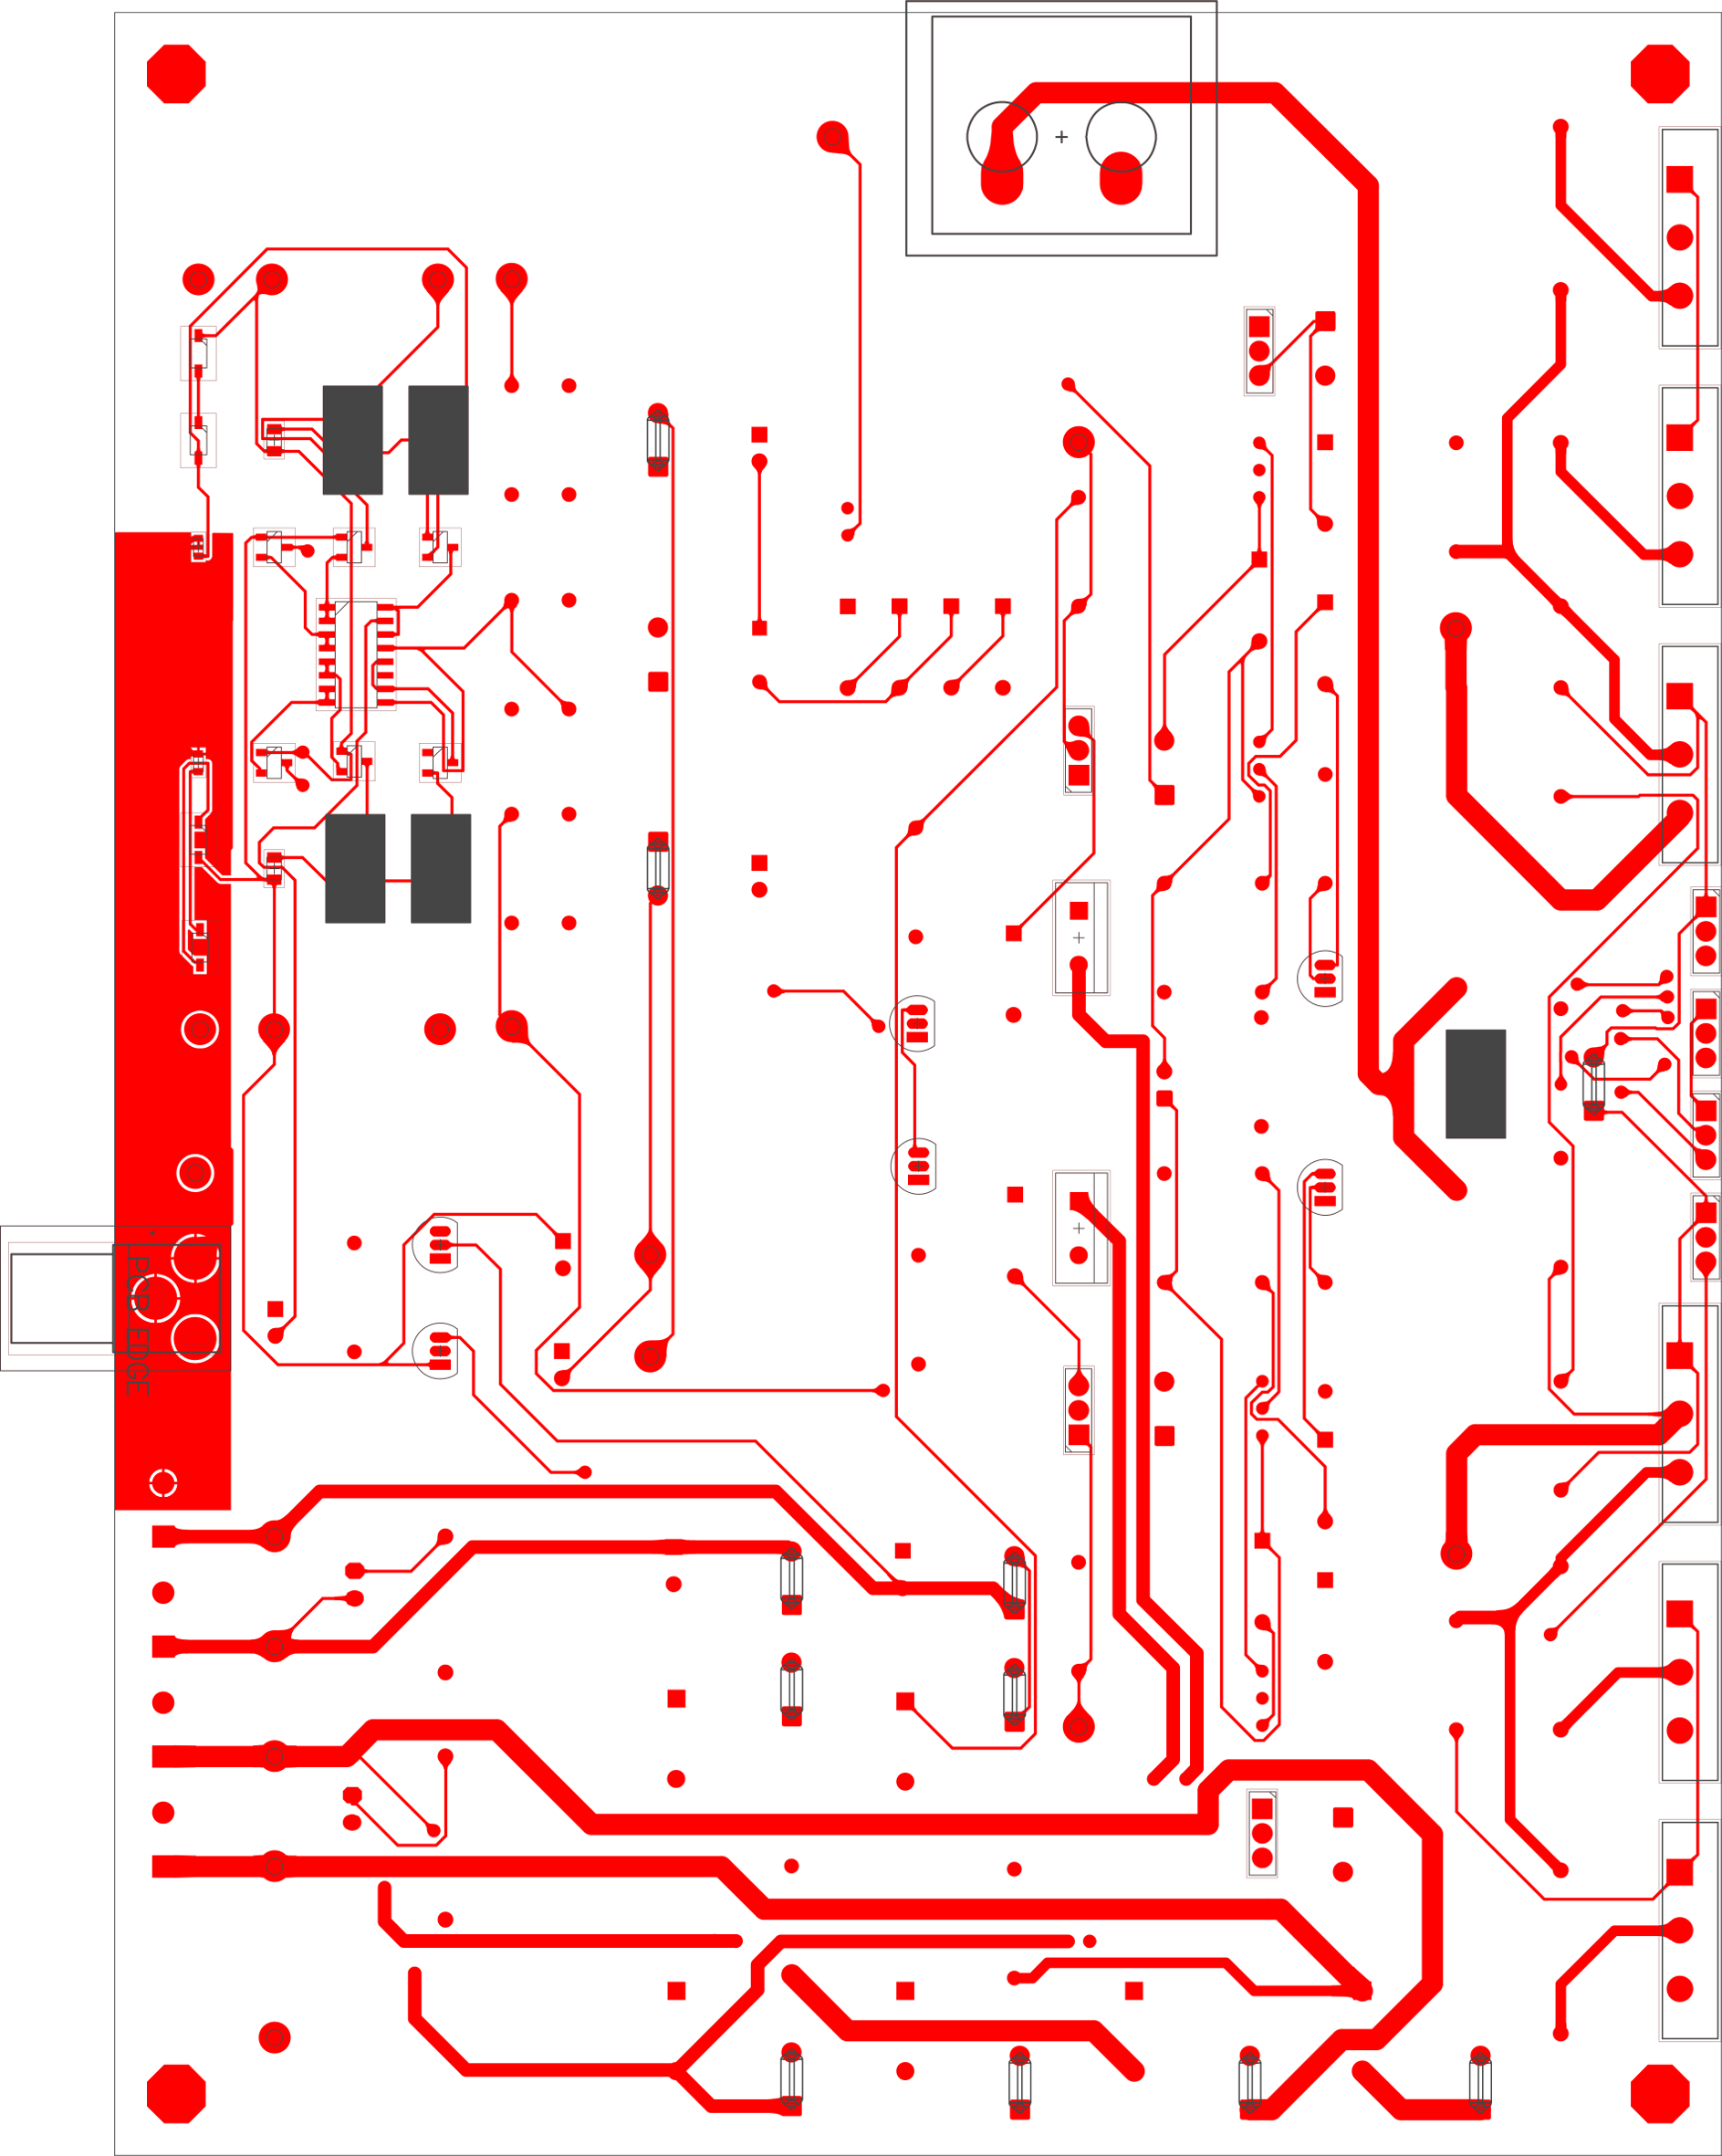
\includegraphics[height=200mm, angle=0]{img/PCB/layers/amplifier/top-copper.png}
    \caption{\footnotesize{Cobre superior}}
    \label{fig:pcb_amp_top_copper}
\end{figure}

\clearpage

\begin{figure}[H]
    \centering
    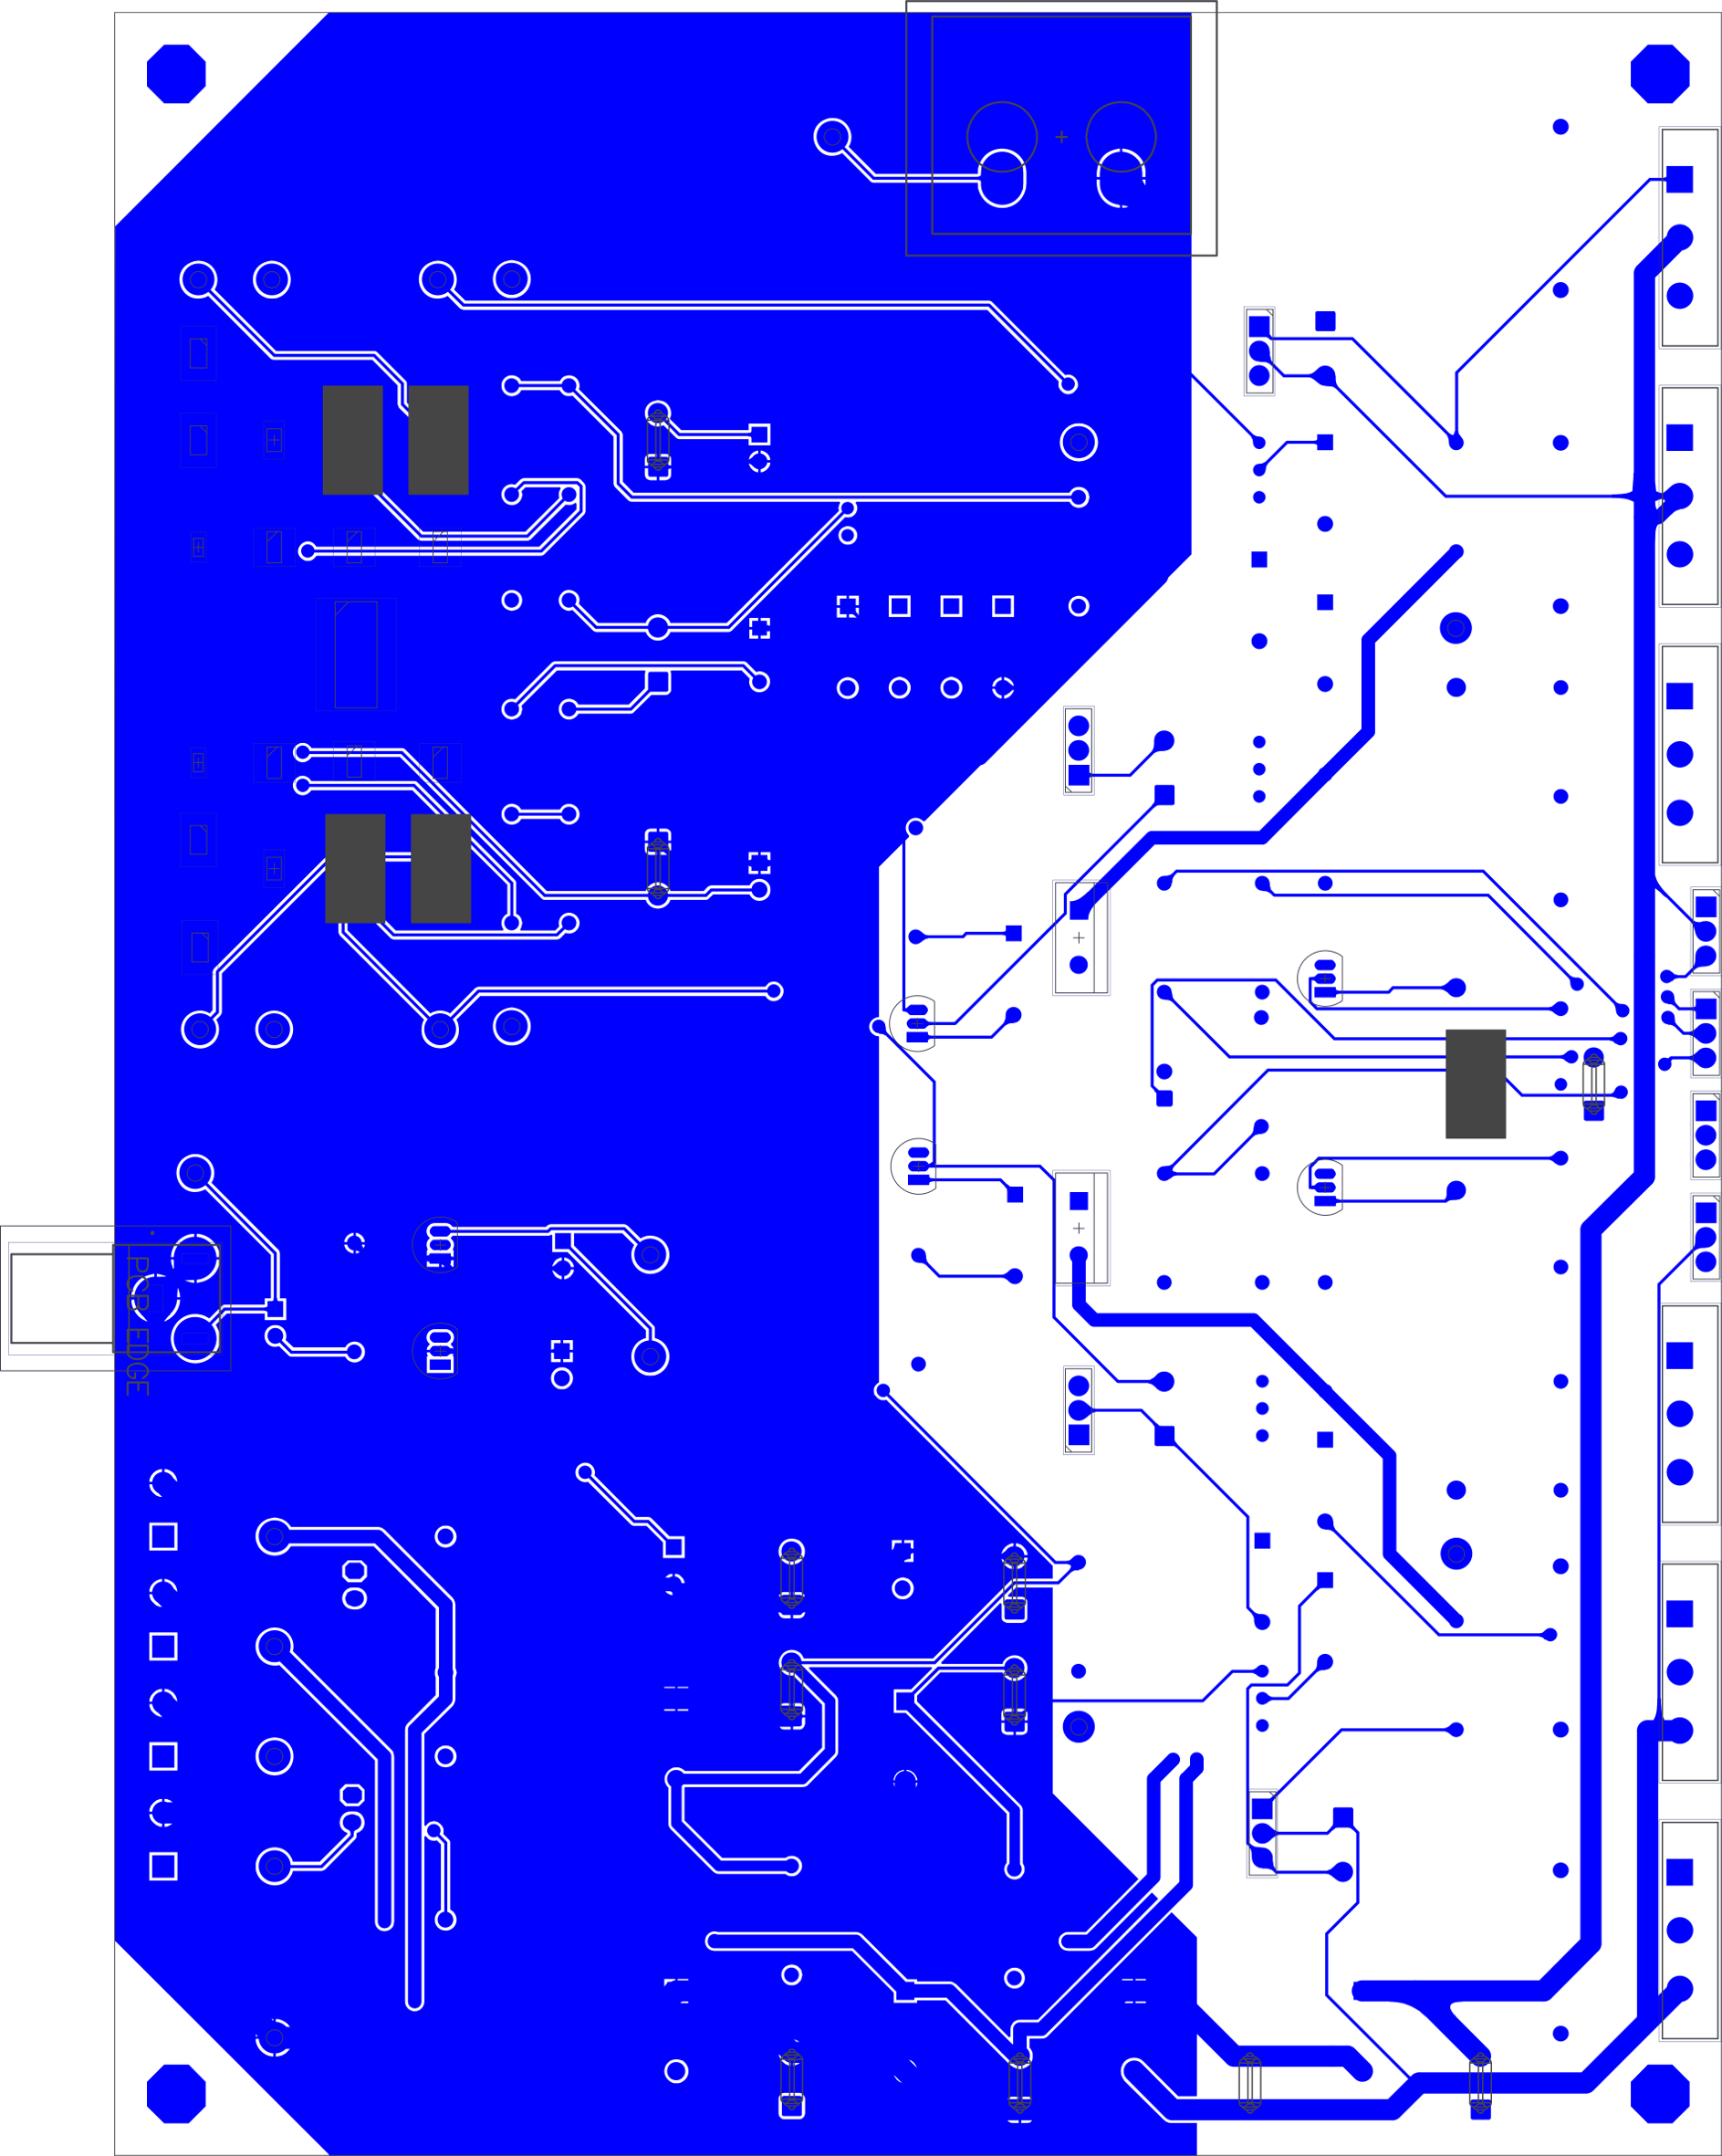
\includegraphics[height=200mm, angle=0]{img/PCB/layers/amplifier/bottom-copper.png}
    \caption{\footnotesize{Cobre inferior}}
    \label{fig:pcb_amp_bottom_copper}
\end{figure}

\clearpage

\begin{figure}[H]
    \centering
    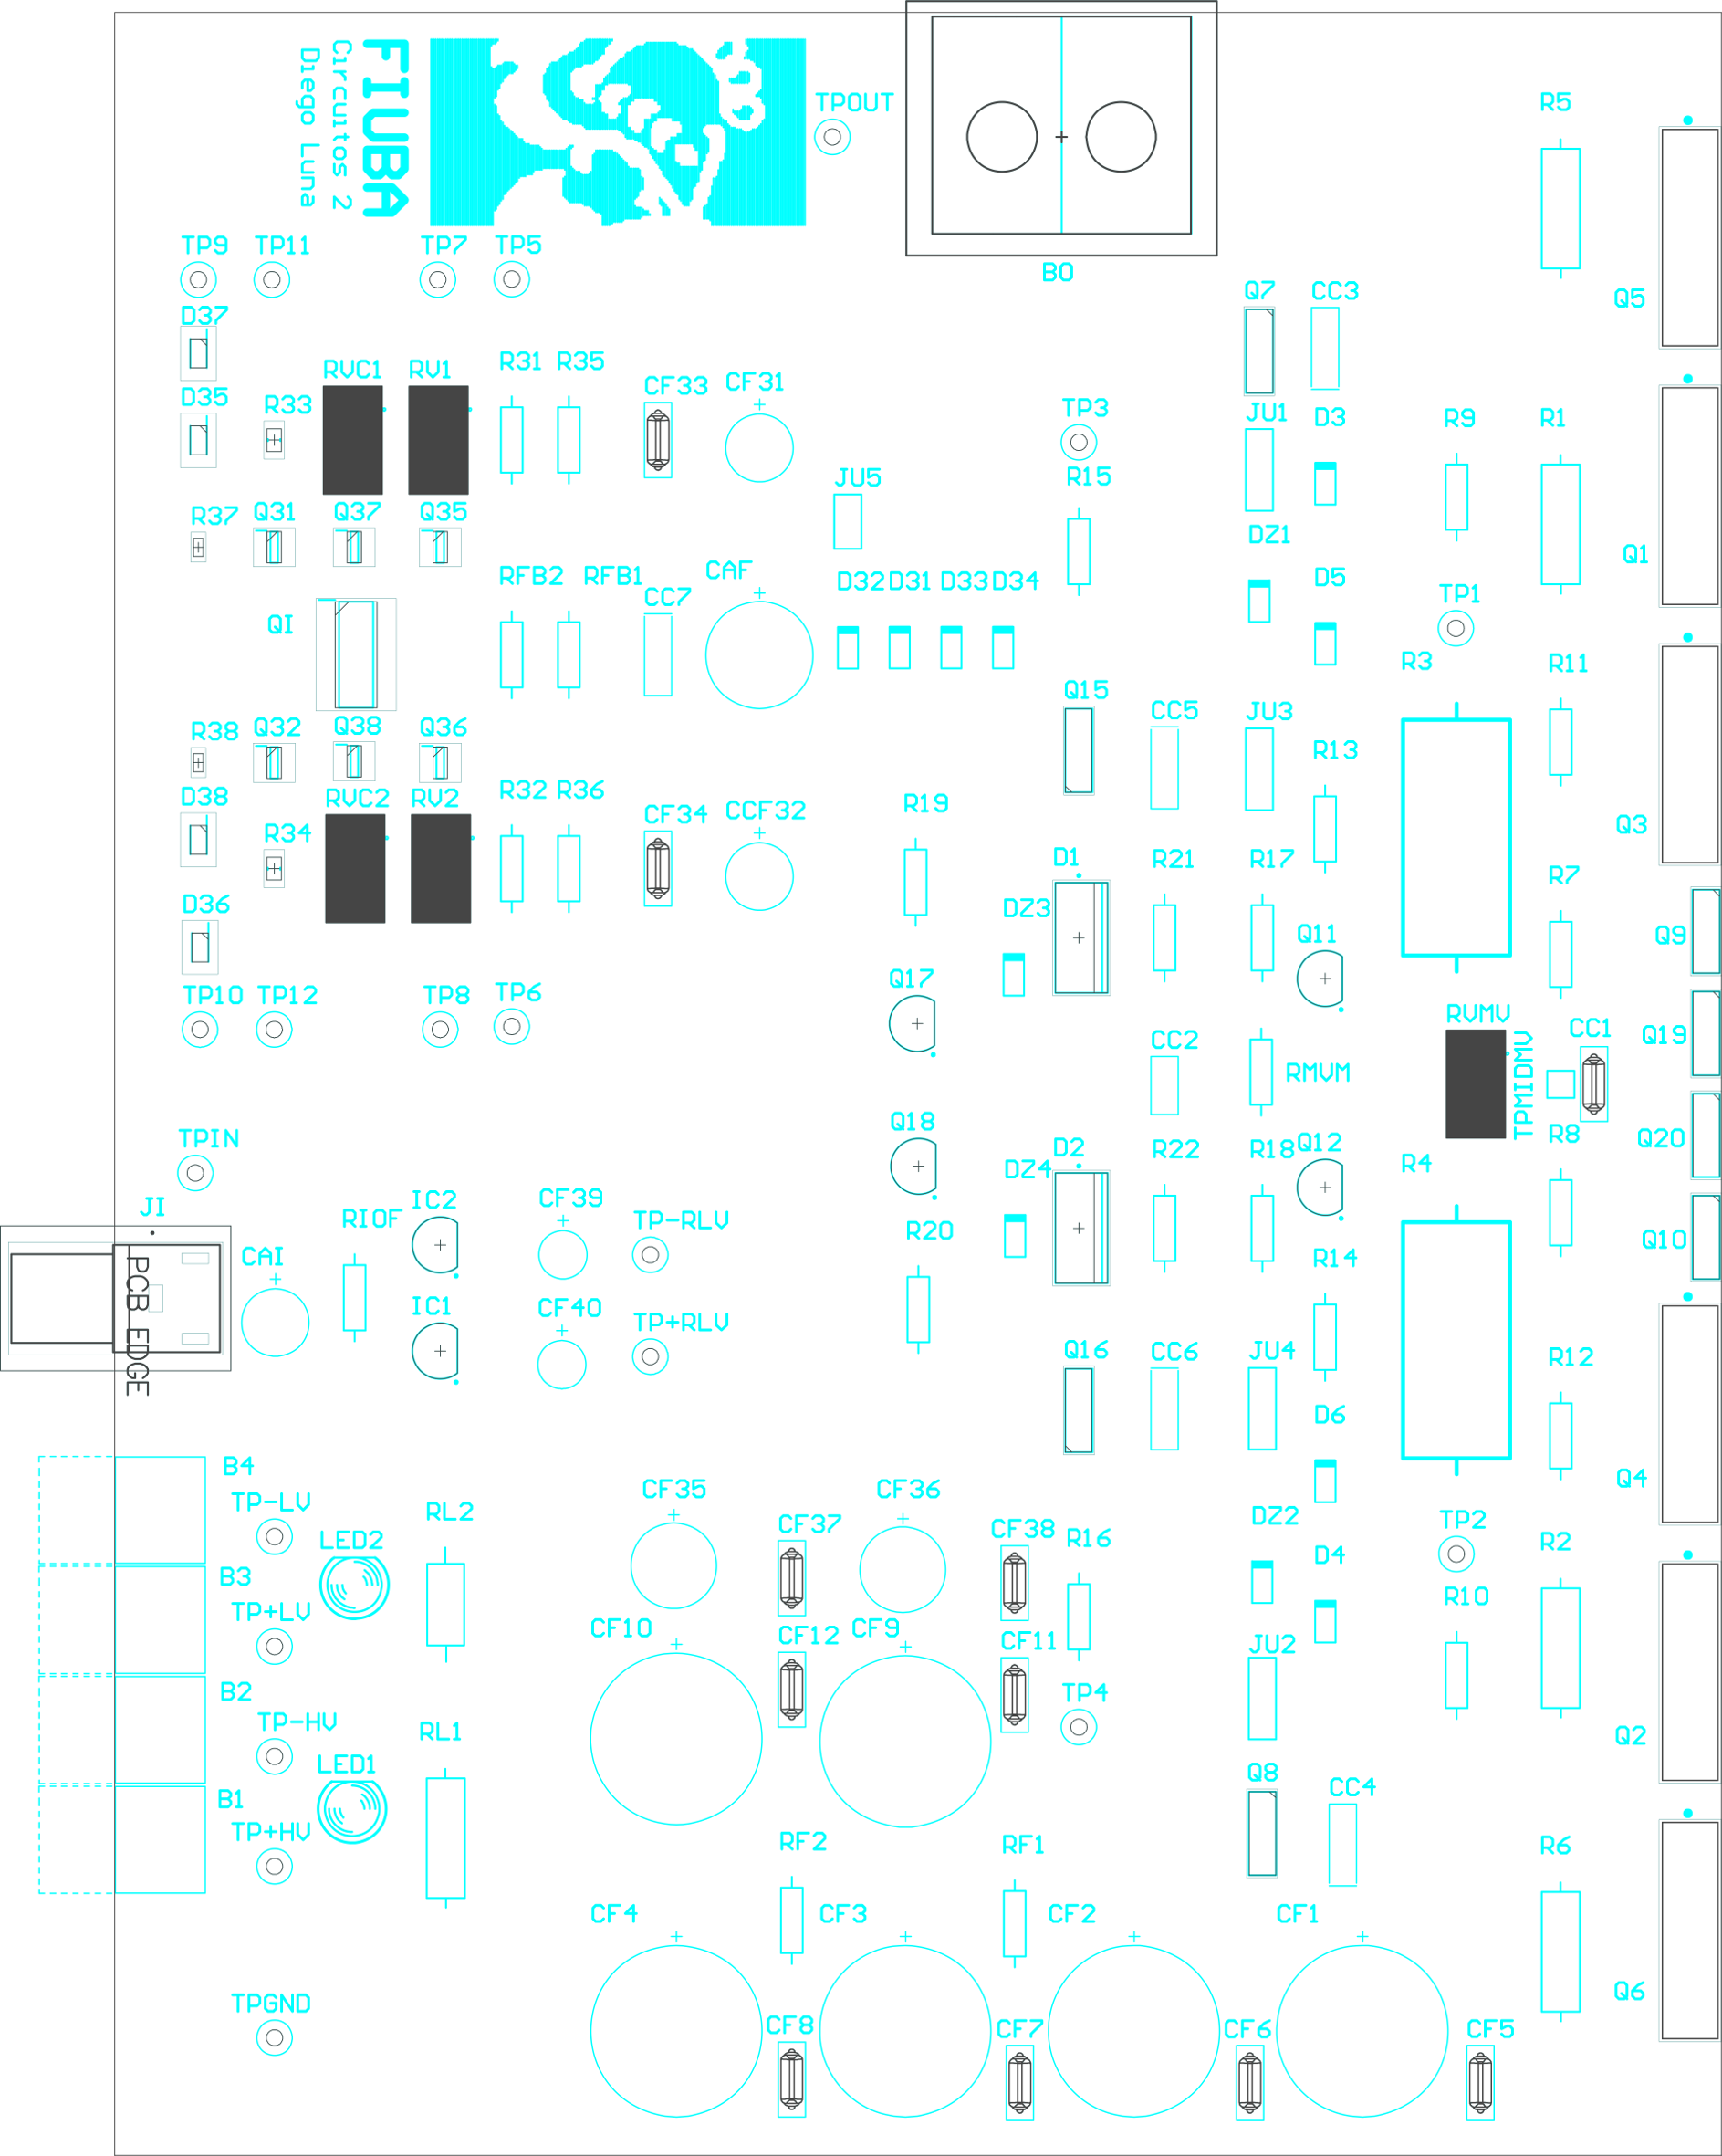
\includegraphics[height=200mm, angle=0]{img/PCB/layers/amplifier/top-overlay.png}
    \caption{\footnotesize{Componentes}}
    \label{fig:pcb_amp_top_overlay}
\end{figure}

\clearpage





\subsection{PCB del pre-amplificador}

En las siguientes páginas se incluyen las capas del PCB del pre-amplificador diseñado en Altium, ver archivo adjunto, \textbf{\quotemarks{PCBS-3D.pdf}} para una vista 3D interactiva del PCB.

\clearpage

\begin{figure}[H]
    \centering
    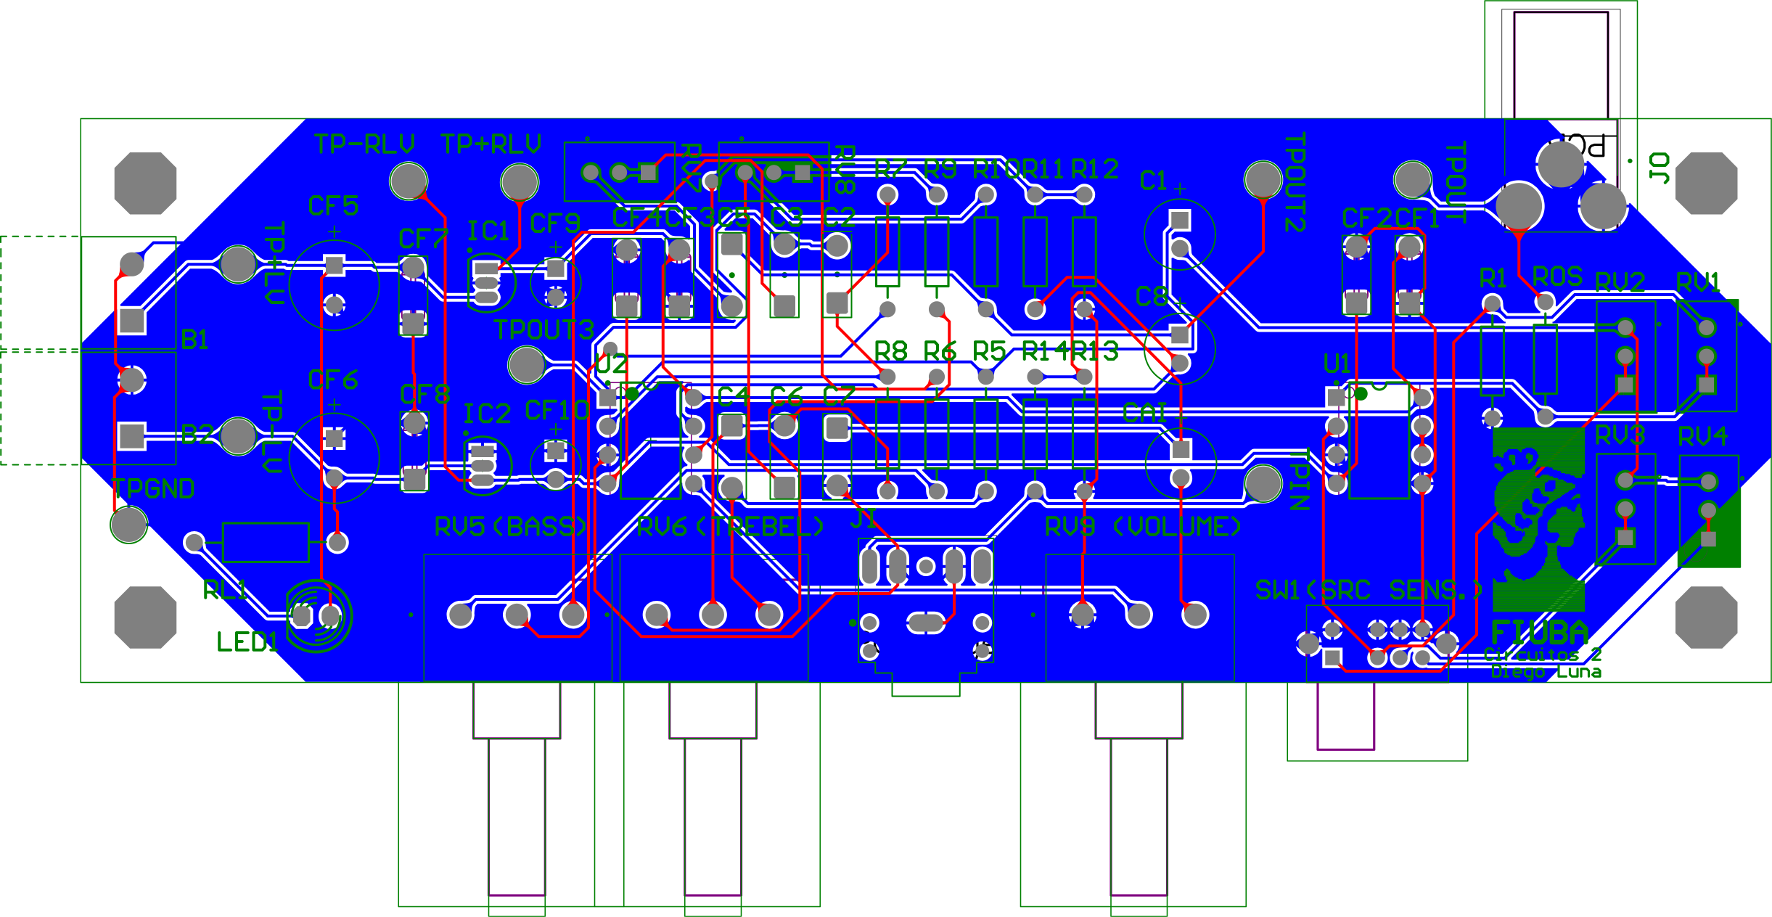
\includegraphics[width=150mm, angle=90]{img/PCB/layers/preamp/all-2D.png}
    \caption{\footnotesize{Todas las capas}}
    \label{fig:pcb_preamp_all}
\end{figure}

\clearpage

\begin{figure}[H]
    \centering
    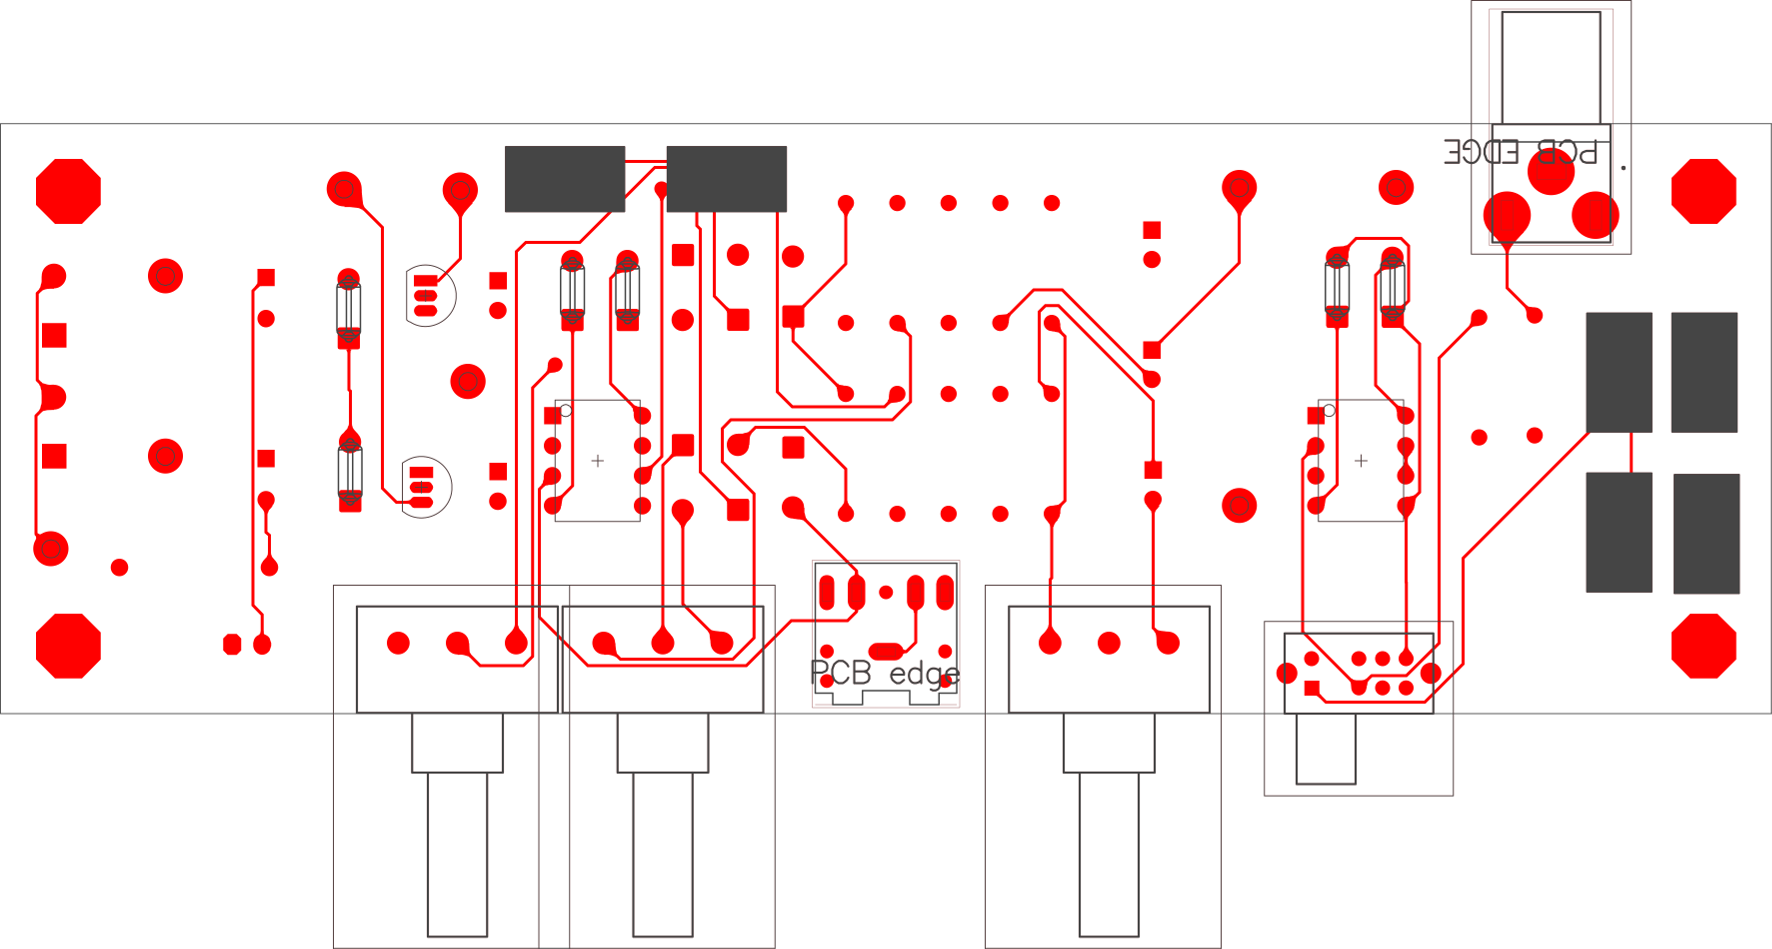
\includegraphics[width=150mm, angle=90]{img/PCB/layers/preamp/top-copper.png}
    \caption{\footnotesize{Cobre superior}}
    \label{fig:pcb_preamp_top_copper}
\end{figure}

\clearpage

\begin{figure}[H]
    \centering
    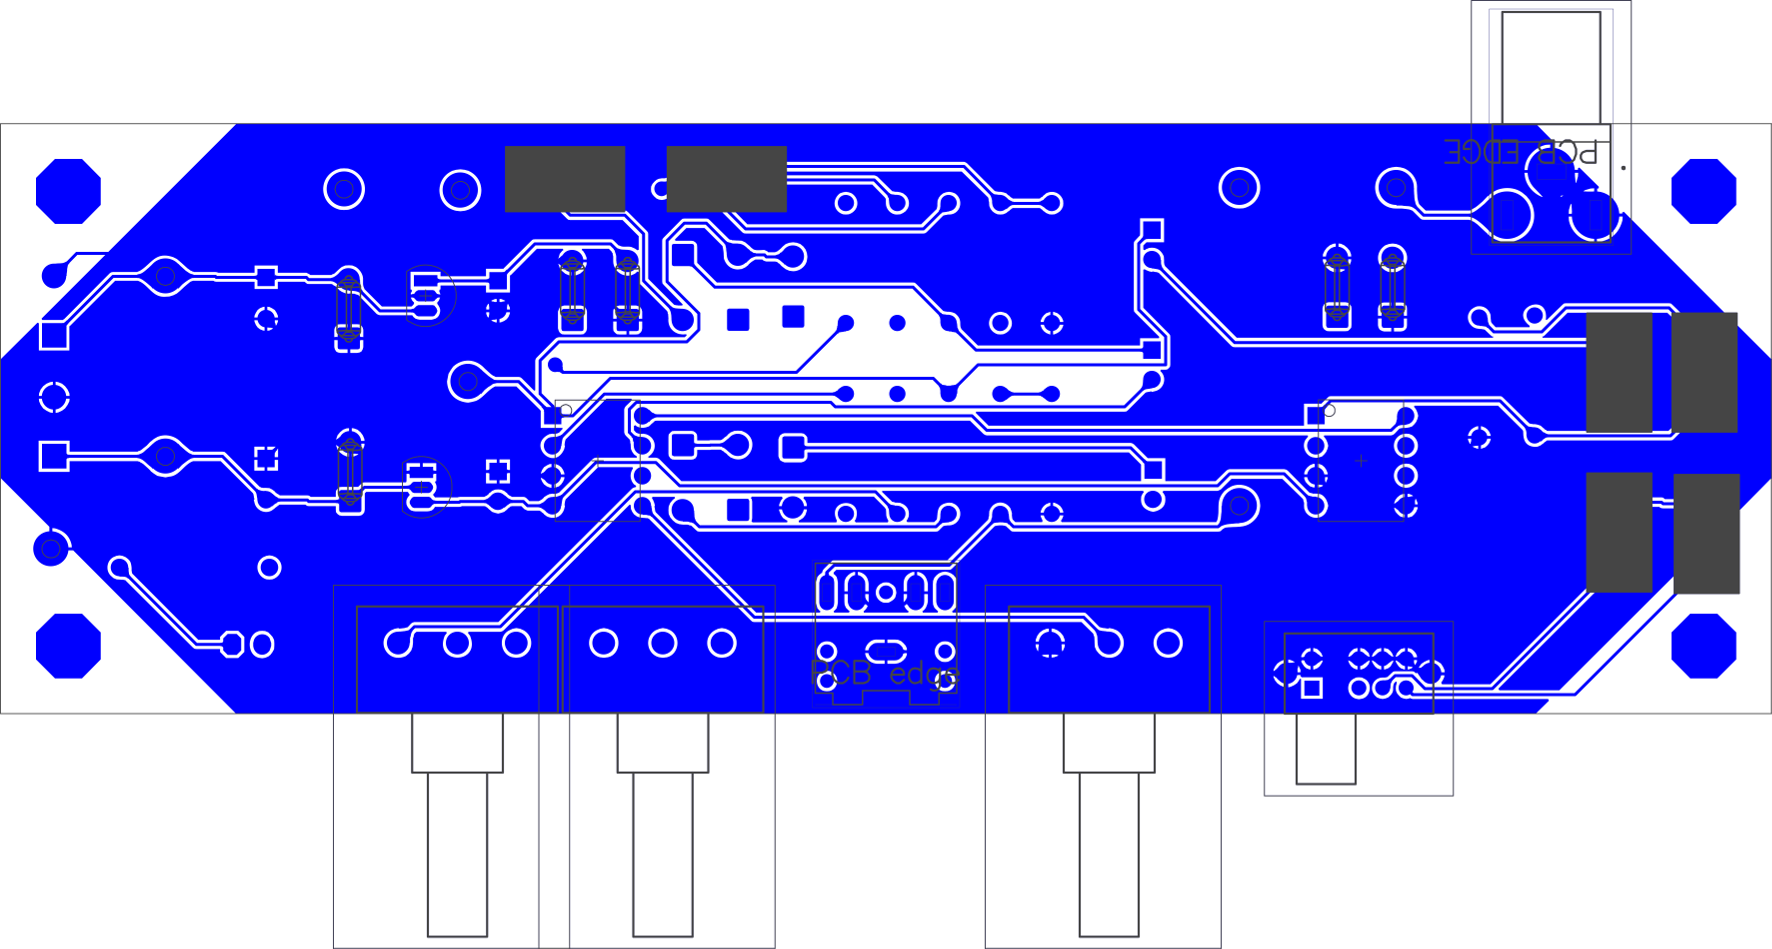
\includegraphics[width=150mm, angle=90]{img/PCB/layers/preamp/bottom-copper.png}
    \caption{\footnotesize{Cobre inferior}}
    \label{fig:pcb_preamp_bottom_copper}
\end{figure}

\clearpage

\begin{figure}[H]
    \centering
    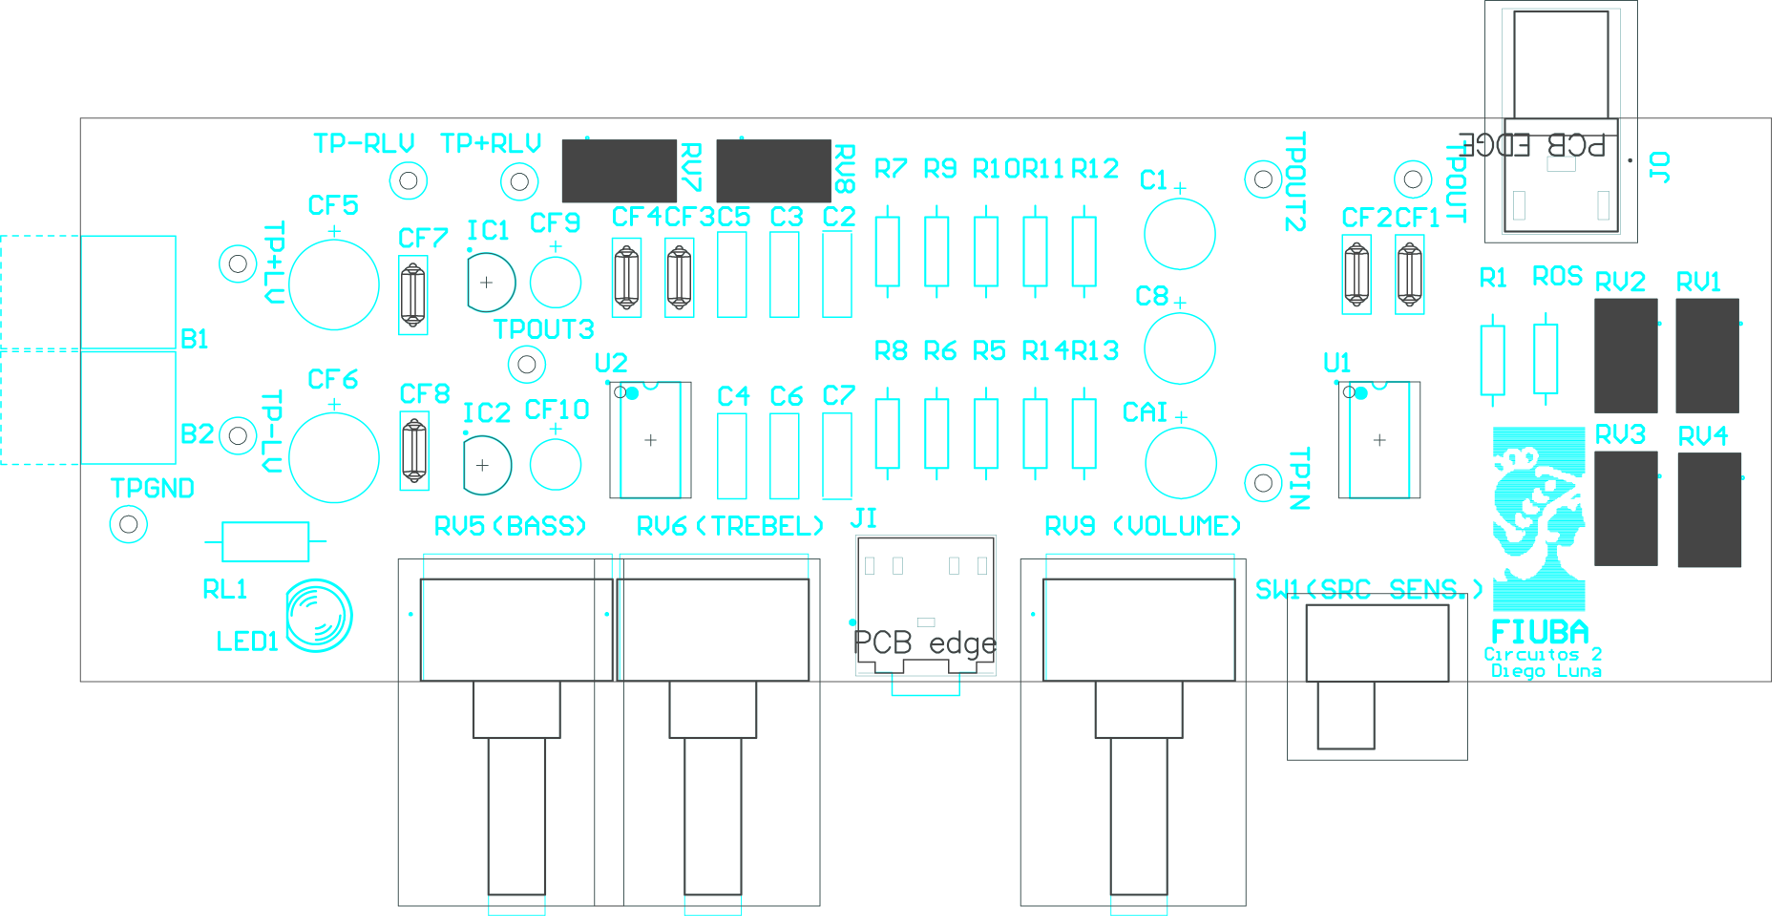
\includegraphics[width=150mm, angle=90]{img/PCB/layers/preamp/top-overlay.png}
    \caption{\footnotesize{Componentes}}
    \label{fig:pcb_preamp_top_overlay}
\end{figure}

\clearpage



\subsection{PCB de la fuente de alimentación}

En las siguientes páginas se incluyen las capas del PCB de la fuente de alimentación diseñada en Altium, ver archivo adjunto, \textbf{\quotemarks{PCBS-3D.pdf}} para una vista 3D interactiva del PCB.

\clearpage

\begin{figure}[H]
    \centering
    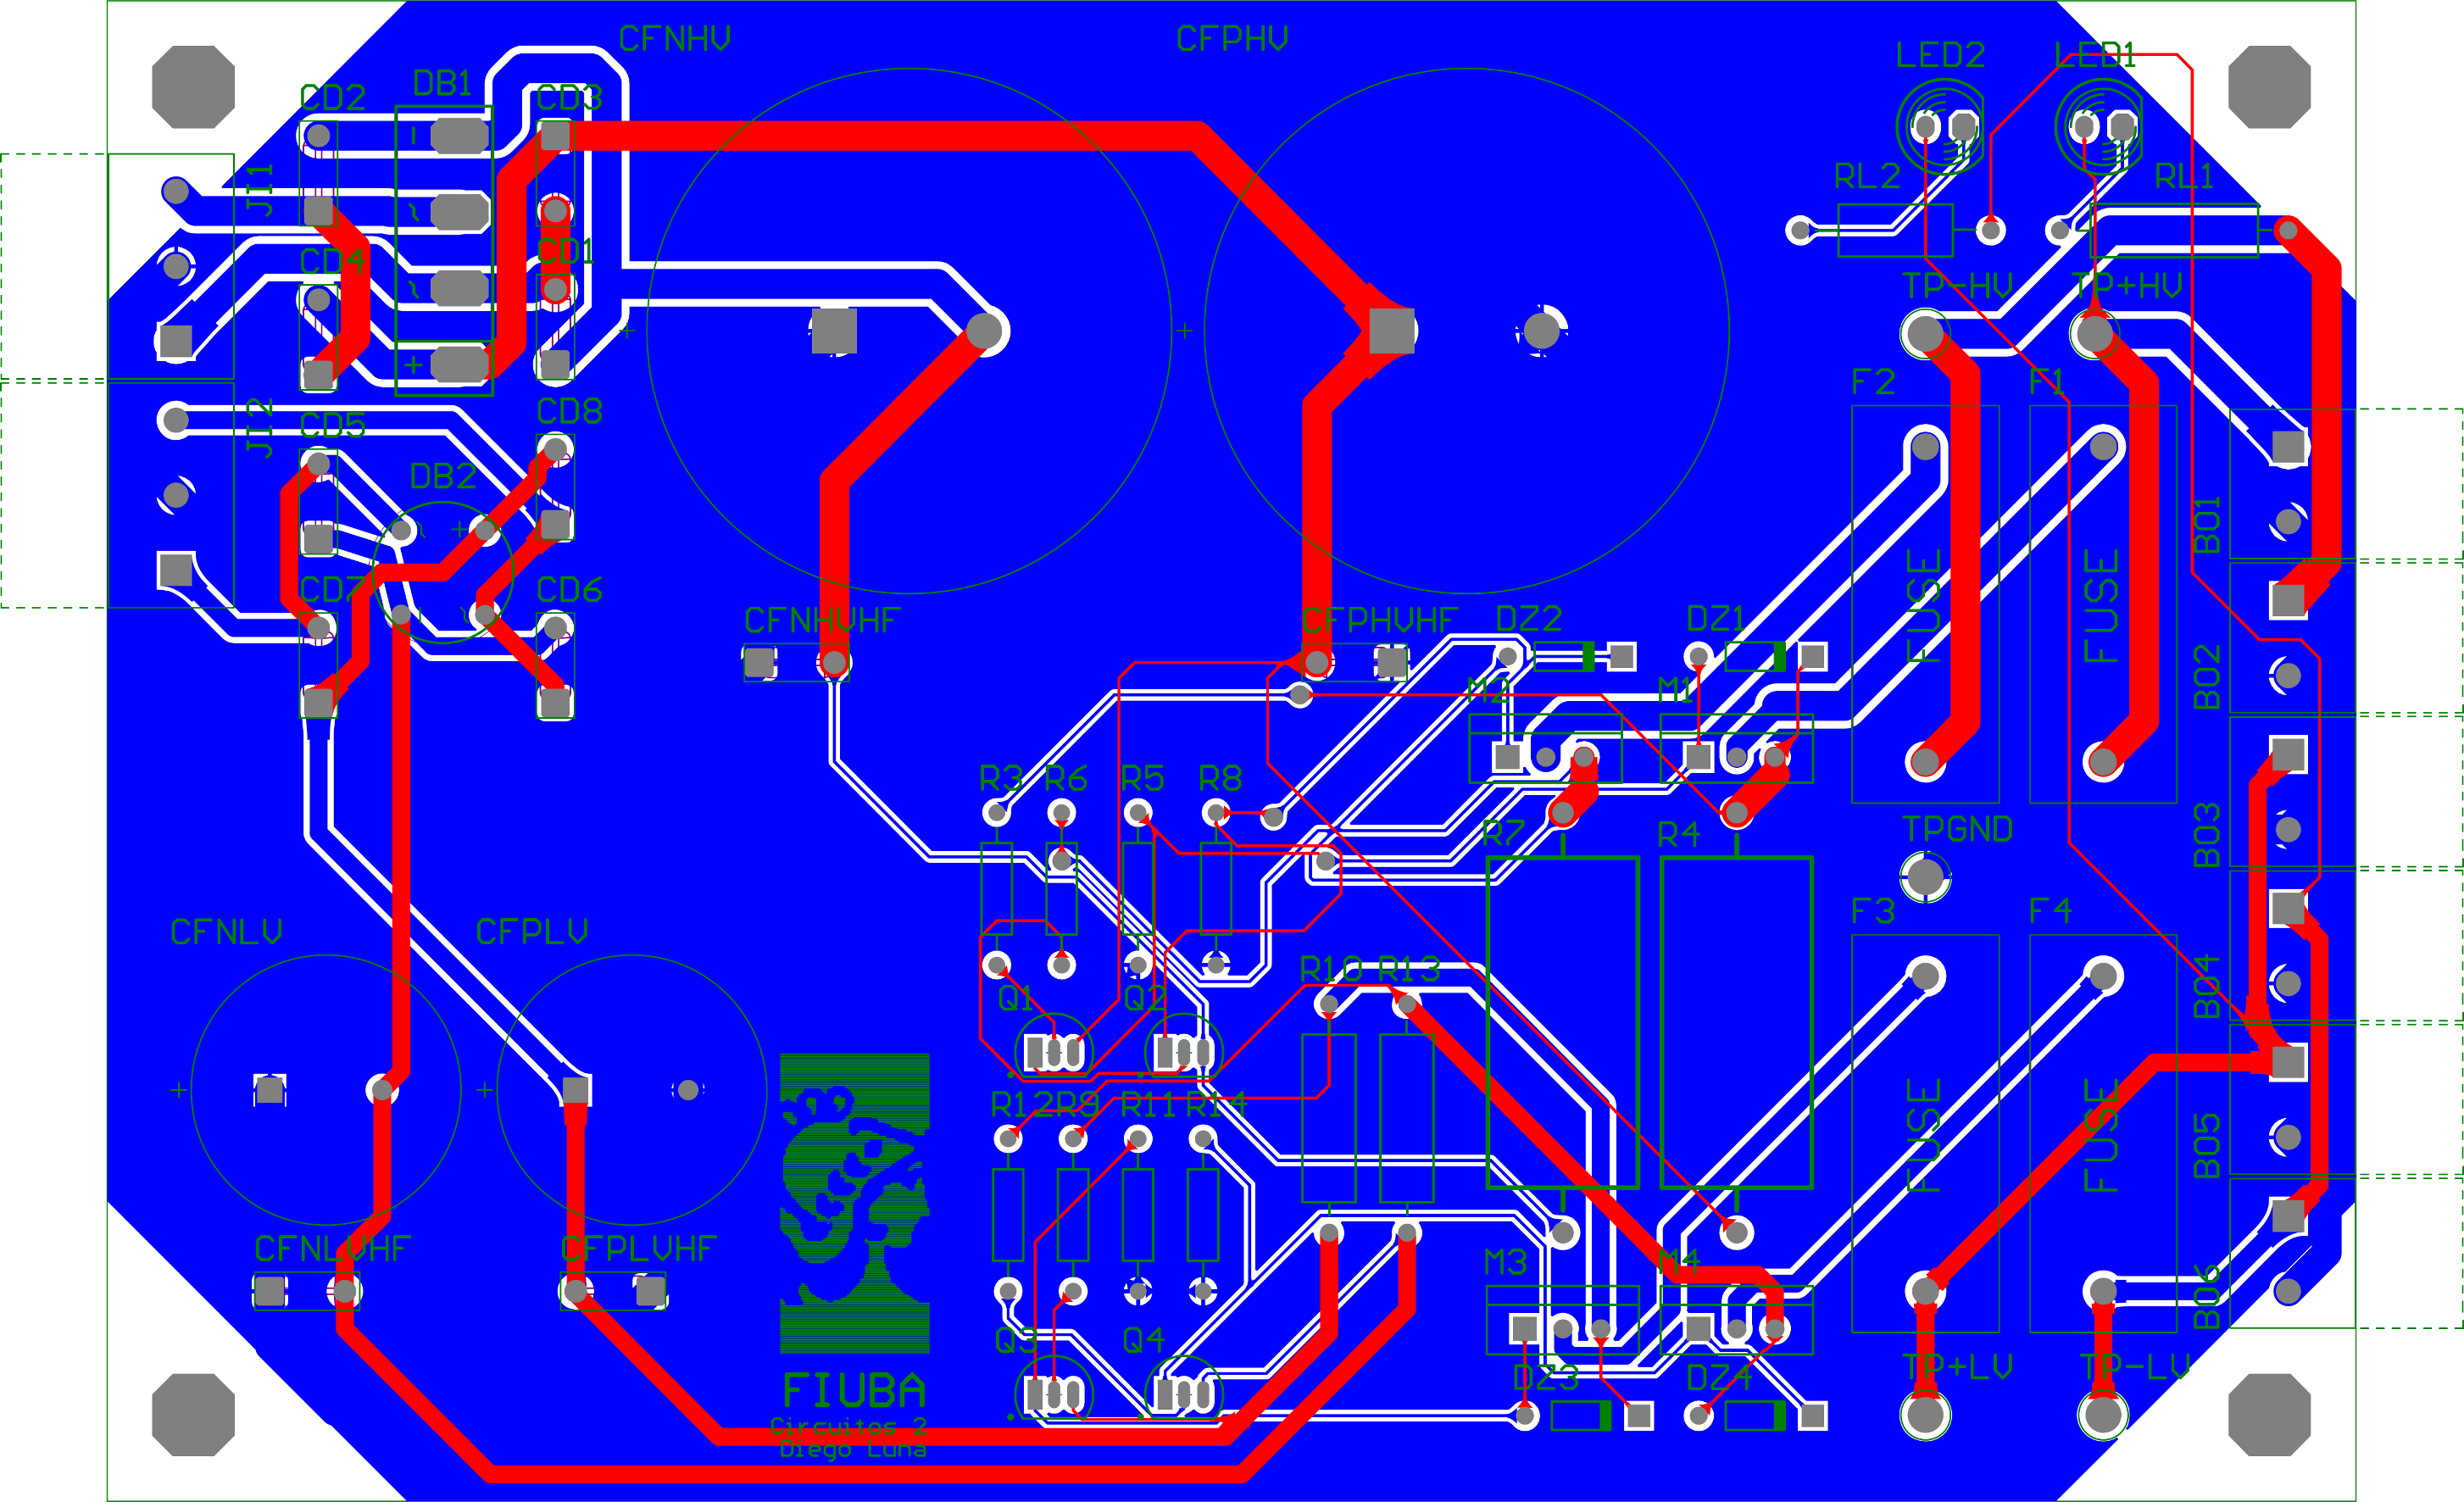
\includegraphics[width=150mm, angle=90]{img/PCB/layers/power_supply/all-2D.png}
    \caption{\footnotesize{Todas las capas}}
    \label{fig:pcb_preamp_all}
\end{figure}

\clearpage

\begin{figure}[H]
    \centering
    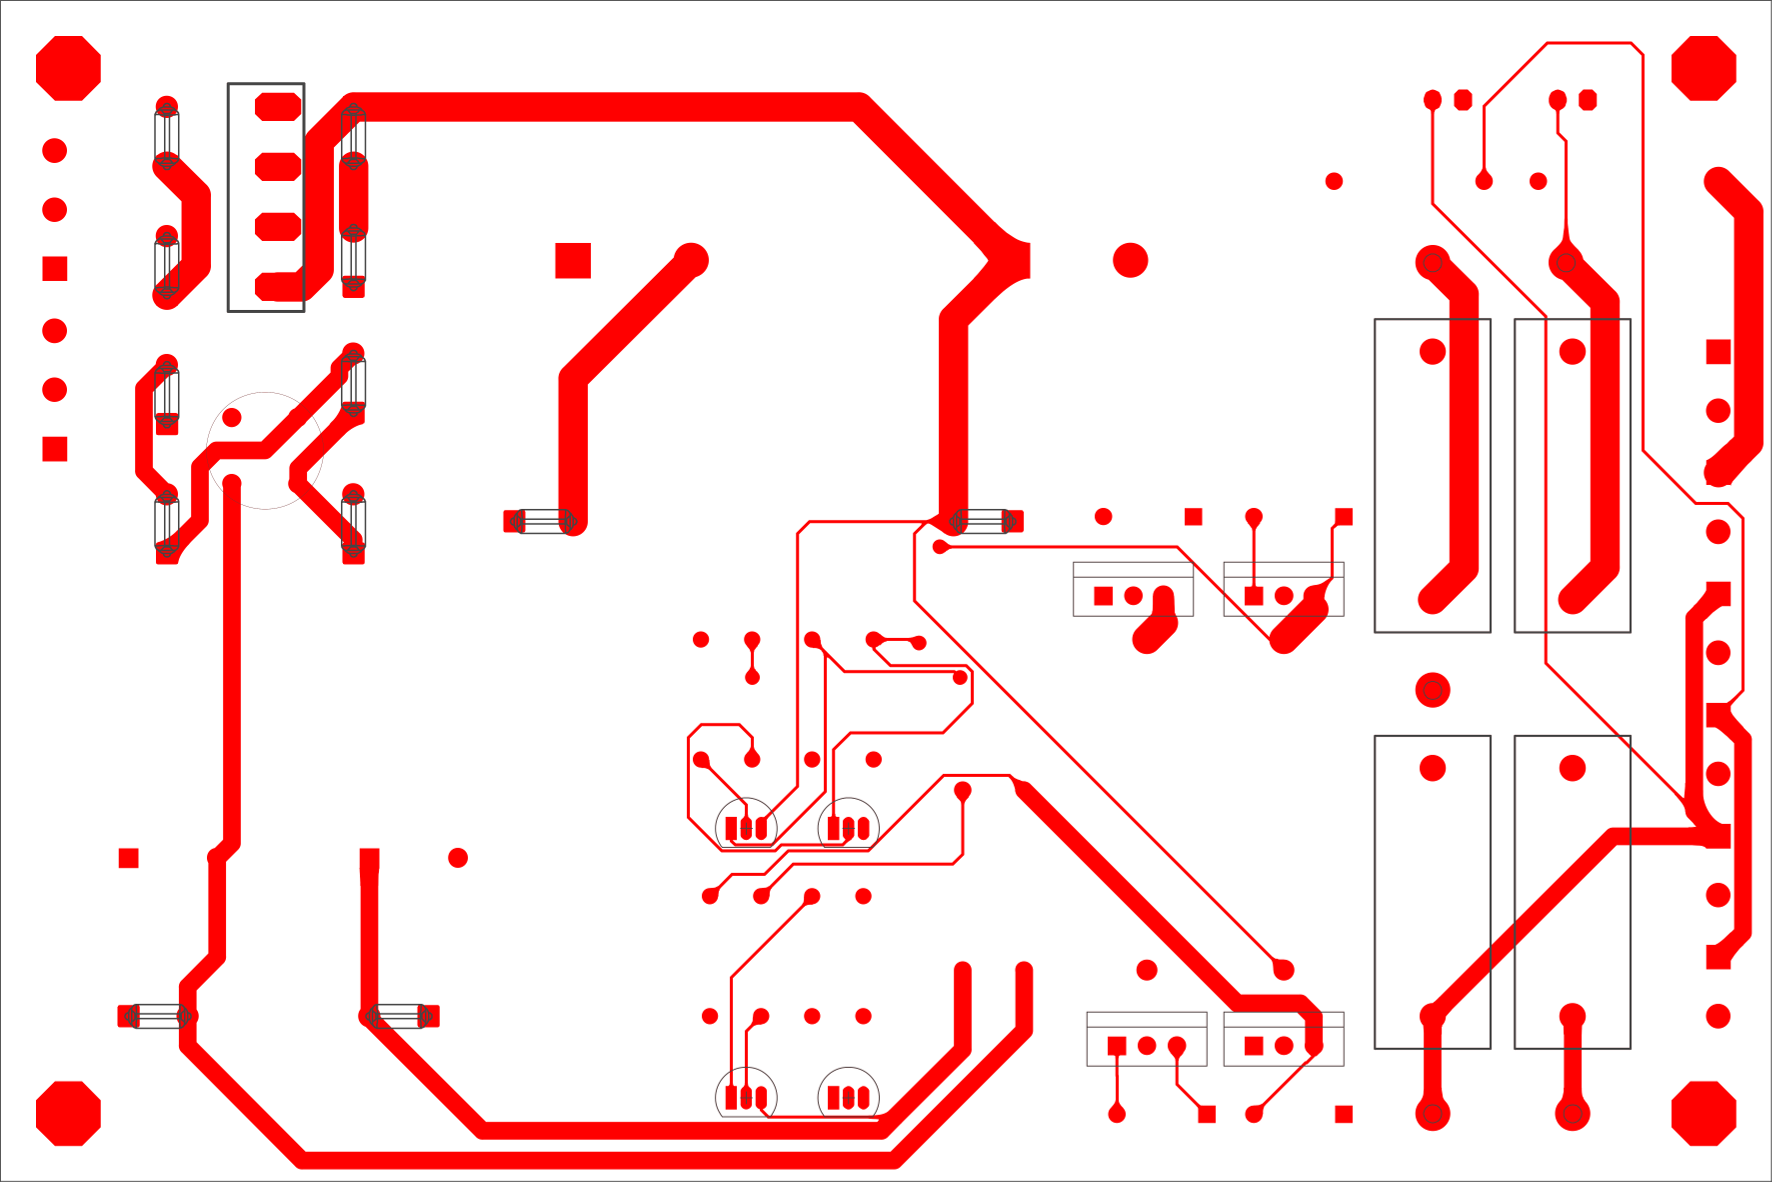
\includegraphics[width=150mm, angle=90]{img/PCB/layers/power_supply/top-copper.png}
    \caption{\footnotesize{Cobre superior}}
    \label{fig:pcb_preamp_top_copper}
\end{figure}

\clearpage

\begin{figure}[H]
    \centering
    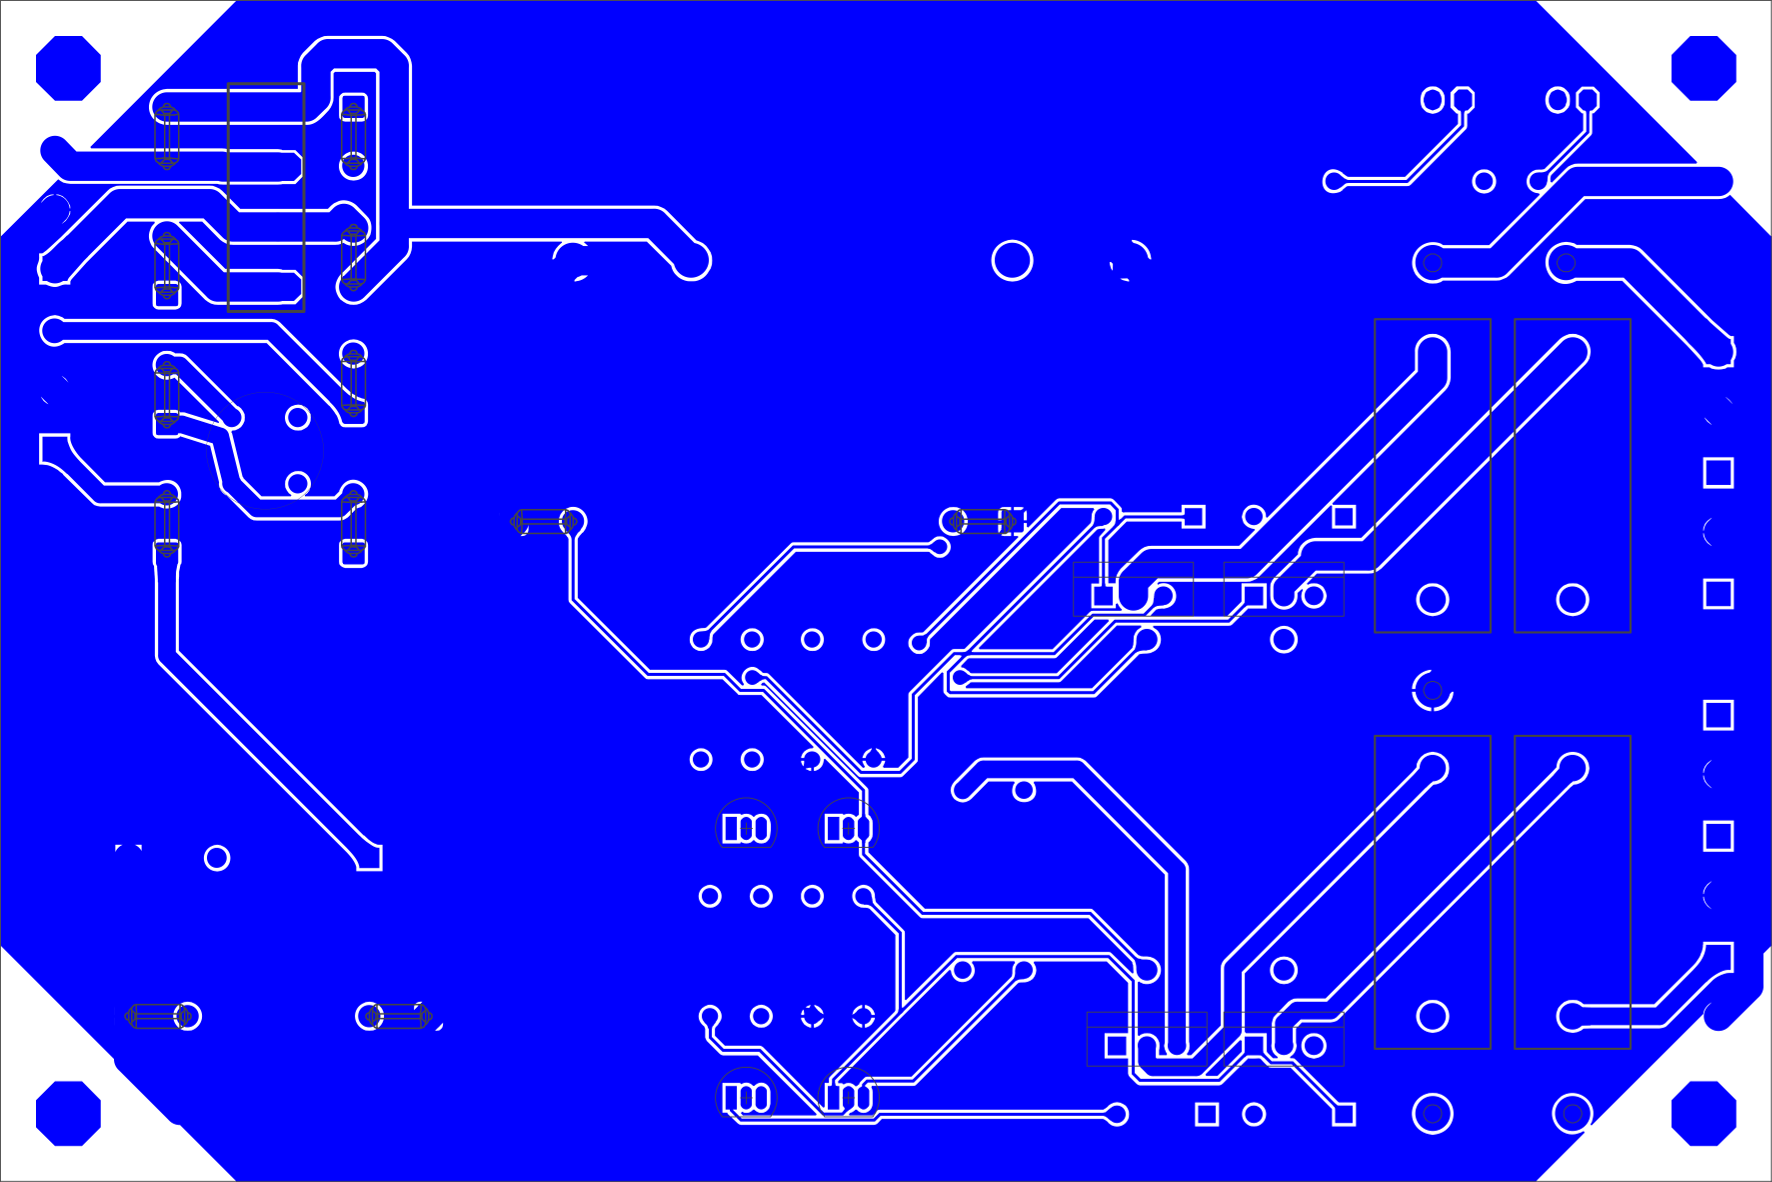
\includegraphics[width=150mm, angle=90]{img/PCB/layers/power_supply/bottom-copper.png}
    \caption{\footnotesize{Cobre inferior}}
    \label{fig:pcb_preamp_bottom_copper}
\end{figure}

\clearpage

\begin{figure}[H]
    \centering
    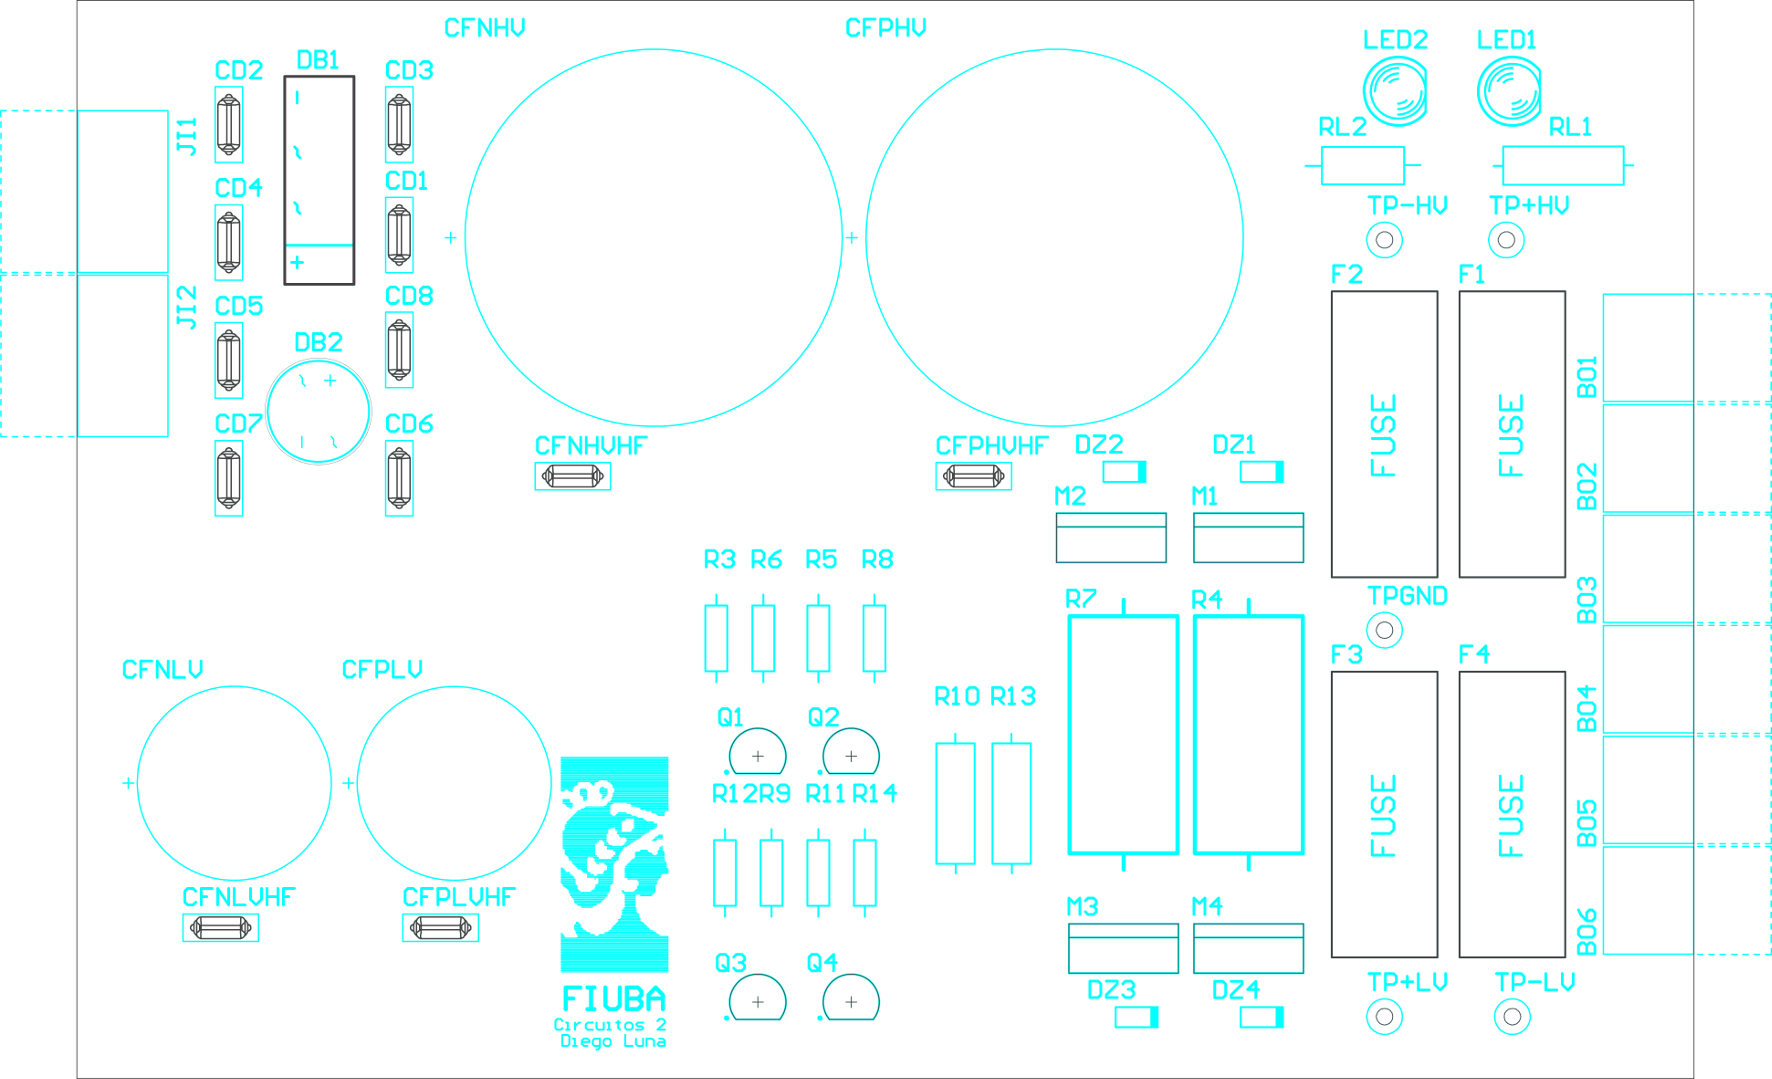
\includegraphics[width=150mm, angle=90]{img/PCB/layers/power_supply/top-overlay.png}
    \caption{\footnotesize{Componentes}}
    \label{fig:pcb_preamp_top_overlay}
\end{figure}

\clearpage

















\clearpage
%\\\\\\\\\\\\\\\\\\\\\\\\\\\


%\\\\\\\\\\\\\\\\\\\\\\\\\\\
\section{Disipación de calor}
\resetallcounters

\label{sec:disipadores}
\begin{figure}[H]
    \centering
    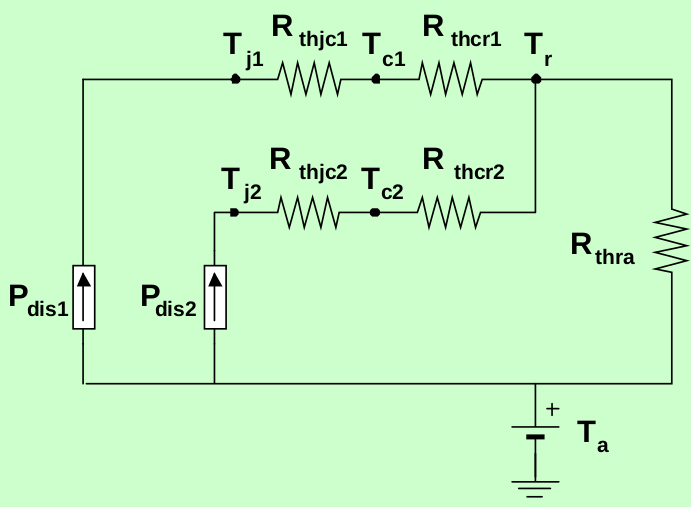
\includegraphics[height=0.4\textwidth]{img/calculo_disipador.png}
    \caption{Modelo térmico estacionario.}
    \label{fig:disipadores}
\end{figure}

En el peor caso, los transistores de potencia \textbf{2SC5200} de la etapa de salida y su par complementario \textbf{2SA1943} disipan cada uno $18 \si[per-mode=symbol]{\watt}$, ya que los mismos se utilizan en paralelo.

\begin{equation*}
T_r = R_{thra} * (P_{dis1}+P_{dis2}) + T_a
\end{equation*}

\begin{equation*}
T_r = T_{juntura_{N}} - (R_{t_{j-case}}+R_{t_{c-heat}})*P_{disN}
\end{equation*}

\begin{equation*}
T_r = 130 \si[per-mode=symbol]{\celsius} - (0.85 \si[per-mode=symbol]{\celsius\per\watt} + 0.1 \si[per-mode=symbol]{\celsius\per\watt})*(18*2 \si[per-mode=symbol]{\watt}) = 95.8 \si[per-mode=symbol]{\celsius}
\end{equation*}

\begin{equation*}
95.8 \si[per-mode=symbol]{\celsius} = R_{thra}*(18*2*2 \si[per-mode=symbol]{\watt}) + 40 \si[per-mode=symbol]{\celsius}
\end{equation*}

\begin{equation*}
R_{tha} = 0.77 \si[per-mode=symbol]{\celsius\per\watt}
\end{equation*}

En la  parte interna de la etapa de salida, tenemos que en el peor caso se disipan $3.25 \si[per-mode=symbol]{\watt}$ por cada transistor. Haciendo las mismas cuentas con otros valores.


\begin{equation*}
T_r = 120 \si[per-mode=symbol]{\celsius} - (6.25 \si[per-mode=symbol]{\celsius\per\watt} + 0.1 \si[per-mode=symbol]{\celsius\per\watt})*(3.25 \si[per-mode=symbol]{\watt}) = 99.36 \si[per-mode=symbol]{\celsius}
\end{equation*}

\begin{equation*}
R_{tha} = 9.13 \si[per-mode=symbol]{\celsius\per\watt}
\end{equation*}

\paragraph{Disipadores elegidos:}

Para la parte externa de la salida \textbf{ZD-23} $0.65 \si[per-mode=symbol]{\celsius\per\watt}$ , elegimos este modelo porque nos da un poco de margen.

\begin{figure}[H]
    \centering
    \includegraphics[height=0.4\textwidth]{img/zd23.jpg}
    \caption{Disipador \textbf{ZD-23}}
    \label{fig:diszd23}
\end{figure}


Para parte interna ZD-14 $2 \si[per-mode=symbol]{\celsius\per\watt}$, si bien solo necesitamos $9 \si[per-mode=symbol]{\celsius\per\watt}$ , elegimos este modelo porque nos da mas margen:

\begin{figure}[H]
    \centering
    \includegraphics[height=0.4\textwidth]{img/zd14.jpg}
    \caption{Disipador \textbf{ZD-14}}
    \label{fig:diszd14}
\end{figure}
\clearpage
%\\\\\\\\\\\\\\\\\\\\\\\\\\\



%\subsection{Diagramas de conexionado}
%El siguiente diagrama muestra como se conectaría la fuente [seccion~\ref{sec:fuente}], el amplificador y el parlante.
%
%\begin{figure}[H]
%\centering
%\includegraphics[width=1\textwidth]{img/integracion/diagrama_completo}
%\caption{Diagrama completo}
%\label{fig:diag_completo} 
%\end{figure}
%
%El la siguiente imagen se muestra el conexionado interno del amplificador en si con los disipadores calculados [seccion~\ref{sec:disipadores}].
%
%\begin{figure}[H]
%\centering
%\includegraphics[width=1\textwidth]{img/integracion/diagrama_interno}
%\caption{Diagrama interno}
%\label{fig:circuito} 
%\end{figure}



%\\\\\\\\\\\\\\\\\\\\\\\\\\\
\section{Observaciones y conclusiones}
\resetallcounters

\subsection{Observaciones y conclusiones}

Cuando empezamos el desarrollo del trabajo práctico intentamos desarrollarlo como si diseñáramos la compensación desde cero, a pesar de que las redes que concluimos que serían necesarias coincidían en la localización con las existentes en el diseño, nos encontramos que el cálculo de los valores requería un desarrollo teórico extenso y una validación iterativa por simulación que se hacia muy complicada en el tiempo disponible, no obstante este primer intento nos sirvió para entender que involucra el diseño de una compensación. \\
Otra cosa en el desarrollo del análisis por simulación es que nos costó un poco en algunos casos ver porque un valor es mejor que otro, al menos por lo que se podía ver en las simulaciones, eso puede ser porque faltan casos que simular, pero ya era bastante extenso como para hacer mas simulaciones. \\
Finalmente, viendo lo justa que queda la compensación para algunos casos, llegamos a la conclusión que sería necesario un análisis por el \textbf{método de Monte Carlo} para garantizar la estabilidad frente a las variaciones de los valores de los componentes, pero nuevamente, el análisis sería demasiado extenso, especialmente dado el tiempo que una simulación estadística puede tomar.
\cleardoublepage
%\\\\\\\\\\\\\\\\\\\\\\\\\\\


%\\\\\\\\\\\\\\\\\\\\\\\\\\\
%Reinicio la cuenta y seteo el estilo de headers y footers.
\pagestyle{bibliostyle}
%\\\\\\\\\\\\\\\\\\\\\\\\\\\

%\\\\\\\\\\\\\\\\\\\\\\\\\\\
\section{Bibliografía}
\resetallcounters

\begin{thebibliography}{9}




\bibitem{Gray_Meyer3}
\Needspace*{7\baselineskip}
\emph{Analysis and Design of Analog Integrated Circuits (3\textsuperscript{rd} Edition)}\\
Author: Paul R. Gray\\
Author: Robert G. Meyer\\
Publisher: John Wiley \& Sons, Inc.; 3\textsuperscript{rd} Edition (Janury 15, 1993)\\
Copyright: \textcopyright \space 1993, John Wiley \& Sons, Inc.\\
ISBN 10: 0471574953\\
Website: \weblink{http://www.wiley.com/WileyCDA/WileyTitle/productCd-EHEP000220.html}{Analysis and Design of Analog Integrated Circuits (3\textsuperscript{rd} Edition)}\\




\bibitem{Gray_Meyer4}
\Needspace*{10\baselineskip}
\emph{Analysis and Design of Analog Integrated Circuits (4\textsuperscript{th} Edition)}\\
Author: Paul R. Gray\\
Author: Paul J. Hurst\\
Author: Stephen H. Lewis\\
Author: Robert G. Meyer\\
Publisher: John Wiley \& Sons, Inc.; 4\textsuperscript{th} Edition (2001)\\
Copyright: \textcopyright \space 2001, John Wiley \& Sons, Inc.\\
ISBN 10: 0471321680\\
ISBN 13: 9780471321682\\
Website: \weblink{http://www.wiley.com/WileyCDA/WileyTitle/productCd-EHEP000220.html}{Analysis and Design of Analog Integrated Circuits (4\textsuperscript{th} Edition)}\\




\bibitem{Gray_Meyer5}
\Needspace*{10\baselineskip}
\emph{Analysis and Design of Analog Integrated Circuits (5\textsuperscript{th} Edition)}\\
Author: Paul R. Gray\\
Author: Paul J. Hurst\\
Author: Stephen H. Lewis\\
Author: Robert G. Meyer\\
Publisher: John Wiley \& Sons, Inc.; 5\textsuperscript{th} Edition (2009)\\
Copyright: \textcopyright \space 2001, John Wiley \& Sons, Inc.\\
ISBN 10: 0470245999\\
ISBN 13: 9780470245996\\
Website: \weblink{https://www.wiley.com/en-ar/Analysis+and+Design+of+Analog+Integrated+Circuits\%2C+5th+Edition-p-9780470245996}{Analysis and Design of Analog Integrated Circuits (5\textsuperscript{th} Edition)}\\



\bibitem{Sedra_Smith_ESP4}
\Needspace*{9\baselineskip}
\emph{Circuitos microelectrónicos (4\textsuperscript{ta} Edición) español}\\
Author: Adel. S. Sedra\\
Author: Kenneth C. Smith\\
Publisher: Oxford, University press; 4\textsuperscript{ta} Edición (2001)\\
Copyright: \textcopyright \space 1999, Oxford, University press México.\\
Original Copyright: \textcopyright \space 1998, 1991, 1987, 1982, Oxford, University press Inc.\\
ISBN 10: 01951166310\\
Website: \weblink{http://www.oup.com/us/companion.websites/0195142519/}{Circuitos microelectrónicos (4\textsuperscript{ta} Edición) español}\\




\bibitem{Sedra_Smith_ENG5}
\Needspace*{8\baselineskip}
\emph{Microelectronic circuits (5\textsuperscript{th} Edition)}\\
Author: Adel. S. Sedra\\
Author: Kenneth C. Smith\\
Publisher: Oxford, University press; 5\textsuperscript{th} Edition (2004)\\
Copyright: \textcopyright \space 2004, 1998, 1991, 1987, 1982, Oxford, University press Inc.\\
ISBN 10: 0195142527\\
Website: \weblink{http://www.oup.com/us/companion.websites/0195142519/}{Microelectronic circuits (5\textsuperscript{th} Edition)}\\





\end{thebibliography}
\cleardoublepage
%\\\\\\\\\\\\\\\\\\\\\\\\\\\

%\\\\\\\\\\\\\\\\\\\\\\\\\\\
%Seteo el stilo de headers y footers.
\pagestyle{allpages}
%\\\\\\\\\\\\\\\\\\\\\\\\\\\

\appendix


\appendixpage
\addappheadtotoc

%\\\\\\\\\\\\\\\\\\\\\\\\\\\


\section{Hojas de datos}



%*********************************************

\subsection{TL431}
\label{datasheet_TL431}
\emph{\textbf{TL431}}\\
\emph{Adjustable precision shunt regulator}\\
\vspace{5pt}
Manufacturer page:	\weblink{http://www.ti.com/product/TL431}{http://www.ti.com/product/TL431}\\

Manufacturer Datasheet:	\weblink{http://www.ti.com/lit/gpn/tl431}{http://www.ti.com/lit/gpn/tl431}\\


\subsection{TL082}
\label{datasheet_TL082}
\emph{\textbf{TL082}}\\
\emph{Dual High Slew Rate JFET-Input Operational Amplifier}\\
\vspace{5pt}
Manufacturer page:	\weblink{http://www.ti.com/product/TL082?keyMatch=TL082}{http://www.ti.com/product/TL082?keyMatch=TL082}\\

Manufacturer Datasheet:	\weblink{http://www.ti.com/lit/gpn/tl082}{http://www.ti.com/lit/gpn/tl082}\\


\subsection{BC548}
\label{datasheet_BC548}
\emph{\textbf{BC548}}\\
\emph{NPN Epitaxial Silicon Transistor}\\
\vspace{5pt}
Manufacturer page:	\weblink{https://www.onsemi.com/PowerSolutions/product.do?id=BC548}{https://www.onsemi.com/PowerSolutions/product.do?id=BC548}\\

Manufacturer Datasheet:	\weblink{https://www.onsemi.com/pub/Collateral/BC550-D.pdf}{https://www.onsemi.com/pub/Collateral/BC550-D.pdf}\\


\subsection{BC558}
\label{datasheet_BC558}
\emph{\textbf{BC558}}\\
\emph{PNP Bipolar Transistor}\\
\vspace{5pt}
Manufacturer page:	\weblink{https://www.onsemi.com/PowerSolutions/product.do?id=BC558B}{https://www.onsemi.com/PowerSolutions/product.do?id=BC558B}\\

Manufacturer Datasheet:	\weblink{https://www.onsemi.com/pub/Collateral/BC556B-D.PDF}{https://www.onsemi.com/pub/Collateral/BC556B-D.PDF}\\

\clearpage


\subsection{BD137}
\label{datasheet_BD137}
\emph{\textbf{BD137}}\\
\emph{$1.5 \si[per-mode=symbol]{\ampere}$, $60 \si[per-mode=symbol]{\volt}$ NPN Bipolar Power Transistor}\\
\vspace{5pt}
Manufacturer page:	\weblink{https://www.onsemi.com/PowerSolutions/product.do?id=BD137}{https://www.onsemi.com/PowerSolutions/product.do?id=BD137}\\

Manufacturer Datasheet:	\weblink{https://www.onsemi.com/pub/Collateral/BD135-D.PDF}{https://www.onsemi.com/pub/Collateral/BD135-D.PDF}\\


\subsection{MJE15032}
\label{datasheet_MJE15032}
\emph{\textbf{MJE15032}}\\
\emph{Bipolar Transistor, NPN, $250 \si[per-mode=symbol]{\volt}$, $8.0 \si[per-mode=symbol]{\ampere}$}\\
\vspace{5pt}
Manufacturer page:	\weblink{https://www.onsemi.com/PowerSolutions/product.do?id=MJE15032}{https://www.onsemi.com/PowerSolutions/product.do?id=MJE15032}\\

Manufacturer Datasheet:	\weblink{https://www.onsemi.com/pub/Collateral/MJE15032-D.PDF}{https://www.onsemi.com/pub/Collateral/MJE15032-D.PDF}\\


\subsection{MJE2955}
\label{datasheet_MJE2955}
\emph{\textbf{MJE2955}}\\
\emph{Bipolar Power Transistor, PNP, $10 \si[per-mode=symbol]{\ampere}$, $60 \si[per-mode=symbol]{\volt}$, $75 \si[per-mode=symbol]{\watt}$}\\
\vspace{5pt}
Manufacturer page:	\weblink{https://www.onsemi.com/PowerSolutions/product.do?id=MJE2955T}{https://www.onsemi.com/PowerSolutions/product.do?id=MJE2955T}\\

Manufacturer Datasheet:	\weblink{https://www.onsemi.com/pub/Collateral/MJE2955T-D.PDF}{hhttps://www.onsemi.com/pub/Collateral/MJE2955T-D.PDF}\\


\subsection{Metal film resistor}
\label{datasheet_METALFILMRESISTOR}
\emph{\textbf{Metal film resistor}}\\
\emph{Metal film resistor}\\
\vspace{5pt}
Manufacturer page:	\weblink{https://www.vishay.com/resistors-fixed/metal-film/tab/doclibrary/}{https://www.vishay.com/resistors-fixed/metal-film/tab/doclibrary/}\\



\subsection{Carbon film resistor}
\label{datasheet_CARBONFILMRESISTOR}
\emph{\textbf{Carbon film resistor}}\\
\emph{Carbon film resistor}\\
\vspace{5pt}
Manufacturer page:	\weblink{http://www.vishay.com/resistors-fixed/carbon-film/tab/doclibrary/}{http://www.vishay.com/resistors-fixed/carbon-film/tab/doclibrary/}\\


\clearpage


\subsection{Ceramic capacitor}
\label{datasheet_CERAMIC_CAPACITOR}
\emph{\textbf{Ceramic capacitor}}\\
\emph{Ceramic disk capacitor}\\
\vspace{5pt}
Manufacturer page:	\weblink{https://www.vishay.com/capacitors/ceramic/disc/}{https://www.vishay.com/capacitors/ceramic/disc/}\\


\subsection{Electrolitic Aluminum capacitor}
\label{datasheet_ELECTROLITIC_CAPACITOR}
\emph{\textbf{Electrolitic capacitor}}\\
\emph{Electrolitic aluminum capacitor}\\
\vspace{5pt}
Manufacturer page:	\weblink{https://www.vishay.com/capacitors/aluminum/}{https://www.vishay.com/capacitors/aluminum/}\\










\clearpage
%\\\\\\\\\\\\\\\\\\\\\\\\\\\





\end{document}
